% \iffalse meta-comment
%
% ledmac.dtx
%
% Author: Peter Wilson (CUA) (now at peter.r.wilson@boeing.com)
%
%<*driver>
\documentclass[twoside]{ltxdoc}
\usepackage{graphicx}
\makeatletter
  \@mparswitchfalse
\makeatother
\EnableCrossrefs
\CodelineIndex
%%\OnlyDescription
\renewcommand{\MakeUppercase}[1]{#1}
\pagestyle{headings}
\setcounter{StandardModuleDepth}{1}
\setcounter{IndexColumns}{2}
\begin{document}
  \DocInput{ledmac.dtx}
\end{document}
%</driver>
%
% \fi
%
% \CheckSum{4493}
%
%
% \DoNotIndex{\@,\@@par,\@beginparpenalty,\@empty}
% \DoNotIndex{\@flushglue,\@input}
% \DoNotIndex{\@makefnmark,\@makeother,\@maketitle}
% \DoNotIndex{\@namedef,\@ne,\@spaces,\@tempa}
% \DoNotIndex{\@tempb,\@tempswafalse,\@tempswatrue}
% \DoNotIndex{\@thanks,\@thefnmark,\@topnum}
% \DoNotIndex{\@@,\@elt,\@forloop,\@fortmp,\@gtempa,\@totalleftmargin}
% \DoNotIndex{\",\/,\@ifundefined,\@nil,\@verbatim,\@vobeyspaces}
% \DoNotIndex{\|,\~,\ ,\active,\advance,\aftergroup,\begingroup,\bgroup}
% \DoNotIndex{\mathcal,\csname,\def,\documentstyle,\dospecials,\edef}
% \DoNotIndex{\egroup}
% \DoNotIndex{\else,\endcsname,\endgroup,\endinput,\endtrivlist}
% \DoNotIndex{\expandafter,\fi,\fnsymbol,\futurelet,\gdef,\global}
% \DoNotIndex{\hbox,\hss,\if,\if@inlabel,\if@tempswa,\if@twocolumn}
% \DoNotIndex{\ifcase}
% \DoNotIndex{\ifcat,\iffalse,\ifx,\ignorespaces,\index,\input,\item}
% \DoNotIndex{\jobname,\kern,\leavevmode,\leftskip,\let,\llap,\lower}
% \DoNotIndex{\m@ne,\next,\newpage,\nobreak,\noexpand,\nonfrenchspacing}
% \DoNotIndex{\obeylines,\or,\protect,\raggedleft,\rightskip,\rm,\sc}
% \DoNotIndex{\setbox,\setcounter,\small,\space,\string,\strut}
% \DoNotIndex{\strutbox}
% \DoNotIndex{\thefootnote,\thispagestyle,\topmargin,\trivlist,\tt}
% \DoNotIndex{\twocolumn,\typeout,\vss,\vtop,\xdef,\z@}
% \DoNotIndex{\,,\@bsphack,\@esphack,\@noligs,\@vobeyspaces,\@xverbatim}
% \DoNotIndex{\`,\catcode,\end,\escapechar,\frenchspacing,\glossary}
% \DoNotIndex{\hangindent,\hfil,\hfill,\hskip,\hspace,\ht,\it,\langle}
% \DoNotIndex{\leaders,\long,\makelabel,\marginpar,\markboth,\mathcode}
% \DoNotIndex{\mathsurround,\mbox,\newcount,\newdimen,\newskip}
% \DoNotIndex{\nopagebreak}
% \DoNotIndex{\parfillskip,\parindent,\parskip,\penalty,\raise,\rangle}
% \DoNotIndex{\section,\setlength,\TeX,\topsep,\underline,\unskip,\verb}
% \DoNotIndex{\vskip,\vspace,\widetilde,\\,\%,\@date,\@defpar}
% \DoNotIndex{\[,\{,\},\]}
% \DoNotIndex{\count@,\ifnum,\loop,\today,\uppercase,\uccode}
% \DoNotIndex{\baselineskip,\begin,\tw@}
% \DoNotIndex{\a,\b,\c,\d,\e,\f,\g,\h,\i,\j,\k,\l,\m,\n,\o,\p,\q}
% \DoNotIndex{\r,\s,\t,\u,\v,\w,\x,\y,\z,\A,\B,\C,\D,\E,\F,\G,\H}
% \DoNotIndex{\I,\J,\K,\L,\M,\N,\O,\P,\Q,\R,\S,\T,\U,\V,\W,\X,\Y,\Z}
% \DoNotIndex{\1,\2,\3,\4,\5,\6,\7,\8,\9,\0}
% \DoNotIndex{\!,\#,\$,\&,\',\(,\),\+,\.,\:,\;,\<,\=,\>,\?,\_}
% \DoNotIndex{\discretionary,\immediate,\makeatletter,\makeatother}
% \DoNotIndex{\meaning,\newenvironment,\par,\relax,\renewenvironment}
% \DoNotIndex{\repeat,\scriptsize,\selectfont,\the,\undefined}
% \DoNotIndex{\arabic,\do,\makeindex,\null,\number,\show,\write,\@ehc}
% \DoNotIndex{\@author,\@ehc,\@ifstar,\@sanitize,\@title,\everypar}
% \DoNotIndex{\if@minipage,\if@restonecol,\ifeof,\ifmmode}
% \DoNotIndex{\lccode,\newtoks,\onecolumn,\openin,\p@,\SelfDocumenting}
% \DoNotIndex{\settowidth,\@resetonecoltrue,\@resetonecolfalse,\bf}
% \DoNotIndex{\clearpage,\closein,\lowercase,\@inlabelfalse}
% \DoNotIndex{\selectfont,\mathcode,\newmathalphabet,\rmdefault}
% \DoNotIndex{\bfdefault}
%
% ^^A PW {\catcode`\$=9
% ^^A PW \gdef\fileversion{ $Revision:   3.16  $ }
% ^^A PW \gdef\filedate{ $Date:   19 Jul 1994 11:17:04  $ }}
% ^^A PW \def\docdate{30 April 1994}
% \def\fileversion{v0.1}
% \def\filedate{2003/04/01}
% \hyphenation{man-u-script man-u-scripts}
%
% \newcommand{\Lpack}[1]{\textsf{#1}}
% \newcommand{\Lclass}[1]{\textsf{#1}}
% \newcommand{\ledmac}{ledmac}
% \newcommand{\edmac}{\texttt{EDMAC}}
% \newcommand{\PWcomment}[1]{}
% \newenvironment{PW}{\itshape}{}
% \renewenvironment{PW}{\sffamily}{}
%
% ^^A PW added following as the definitions are at some unknown elsewhere
% \newcommand{\egstart}{}
% \newcommand{\egmid}{}
% \newcommand{\egend}{}
%
% \renewcommand{\egstart}{%
%    \par
%    \begingroup
%    \centering
%    \begin{minipage}{0.45\textwidth}}
% \renewcommand{\egmid}{%
%    \end{minipage}\begin{minipage}{0.45\textwidth}}
% \renewcommand{\egend}{%
%    \end{minipage}\par\endgroup}
%
% \title{\Lpack{\ledmac} \\
%        A brave but perhaps doomed attempt to port \texttt{EDMAC}
%        to LaTeX\thanks{This file has version number \fileversion, 
%                        last revised \filedate.}}
%
% \author{%
% Peter Wilson\thanks{%
% Catholic University of America 
% (Now at \texttt{peter.r.wilson@boeing.com})} \\[1.5\baselineskip]
% {\small based on the original work by} \\[1.5\baselineskip]
% John Lavagnino and Dominik Wujastyk
% }
%
%  \iffalse     This is a METACOMMENT
%           Everything up to the next `\ fi' (without a blank) will
%           be ignored. This is necessary because `%' may no longer
%           be a comment mark when this file is read in.
%
% The original EDMAC was written by:
% \author{John Lavagnino\thanks{%
%  Department of English and American Literature,
%  Brandeis University,
%  415 South Street,
%  Waltham, MA  02254--9110,  USA.
%  Internet: {\tt lav@binah.cc.brandeis.edu},
%  Bitnet: {\tt lav@brandeis}.}
%  \and Dominik Wujastyk\thanks{%
%  Wellcome Institute for the History of Medicine,
%  183 Euston Road,
%  London NW1 2BE, UK.
%  Internet: {\tt D.Wujastyk@ucl.ac.uk},
%  Bitnet: {\tt dow@harvunxw}.}}
%  \date{}
%
%
%% Macro file `EDMAC' for use with Plain TeX.
%% Copyright (C) 1990, 1991, 1992, 1993, 1994 John Lavagnino and Dominik
%% Wujastyk, all rights reserved.
%
% Copying of this file is authorized only if either
% (1) you make absolutely no changes to your copy, including name, or
% (2) if you do make changes, you name it something other than
%     edmac.tex or edmac.doc
% This restriction helps to ensure that the macro development is orderly.
%
%  HISTORY:
%
% $Log:   C:/EDMAC/VCS/EDMAC.DOV  $
% 
%    Rev 3.16   19 Jul 1994 11:17:04
% o  corrected space bug in \getref@num (thanks to Bernt Karasch);
%    changed documentation of how to use NFSS to point to an external
%    description ed-nfss.tex.
% 
%    Rev 3.15   13 May 1994 18:03:44
% o  added more comment to \morenoexpands;
% o  added example of \printlines after Sanskrit example;
% o  added more info on editions being done with EDMAC;
% o  minor tidying.
% 
%    Rev 3.14   11 May 1994 15:03:04
% o  removed a spurious space from \@lab; corrected a typo in docs.
% 
%    Rev 3.13   11 May 1994 14:01:28
% o   defined \list@clear and \list@create separately;
% o   swapped the subsections on fonts back, so NFSS is described first;
% o   rephrased all sentences with the word "default" to avoid its use.
% 
%    Rev 3.12   11 May 1994 12:03:10
% o  capitalized the footnote and endnote series letters: a-e > A-E.
% 
%    Rev 3.11   10 May 1994 15:19:54
% o  removed the optional braces from the second argument of \text
%    in the examples, and altered the documentation to match.
% 
%    Rev 3.10   10 May 1994 14:31:30
% o  changes to documentation;
% o  made \list@create same as \list@clear;
% o  added \f@encoding and \fontencoding;
% o  corrected \getref@num and \label@parse;
% o  brought the appendix examples more up to date and checked them;
% o  added more cross-references;
% o  added \selectfont to the end of NFSS-\select@@lemmafont.
%
%    Rev 3.9   03 May 1994 11:42:36
% o  Full incorporation of edmacfss.doc. Appropriate changes in
%    documentation. New \morenoexpands macro. New \list@create
%    and \list@clear in anticipation of faster list handling.
%    Numerous running changes.
% 
%    Rev 3.8   14 Apr 1994 12:02:22
% o  revised the cross-referencing macros, which weren't working.
%
%    Rev 3.7   31 Aug 1993 15:57:20
% o  Further changes in response to reviewer's observations. Correct
%    explanation of recursion problem with (some) aliases for \text.
%    Changed several more {\tt ...} strings to "..."; added some
%    \mbox{}s for italic in mathmode (wanted by NFSS2).
%
%    Rev 3.6   27 Aug 1993 16:50:42
% o  made changes as recommended in the TUG publication reviewer's report.
%    Mostly changes to docs; added \edmac@warning.
% o  Added a paragraph to Known Bugs highlighting problem of line breaking
%    in paragraphed footnotes.
%
%    Rev 3.5   23 Mar 1993 15:03:34
% o  added the corrections spotted by Gyula Mayer: some word duplications
%    and important changes to slhh.tex to make it compatible with the
%    current level of edmac.
%
%    Rev 3.4   12 Mar 1993 13:47:32
% o  added appendix material: inclusion of EDMACFSS.DOC and
%    example page of Arabic from Klaus Lagally.
% o  cosmetic changes to some \index entries, and removal of
%    some unnecessary \Make/DeleteShortVerb statements.
%
%    Rev 3.3   11 Mar 1993 12:56:34
% o  John's formatting revisions:
%    Fold long code lines so they don't overrun the measure.
%    Subsubsections changed to paragraphs.
%
%    Rev 3.2   26 Feb 1993 17:55:12
% o  correction to def'n of \@adv: spotted by Klaus Lagally.
%
%    Rev 3.1   25 Feb 1993 15:15:00
% o  small changes to documentation.
%
%    Rev 3.1   25 Feb 1993 12:17:12
% o  small changes to documentation.
%
%    Rev 3.0   25 Jun 1992 12:38:00
%    No change.
%
%    Rev 2.25   25 Jun 1992 12:29:20
% o  cosmetic changes to examples and \ipn@skip use.
%
%    Rev 2.24   22 Jun 1992 13:33:12
% o  cosmetic corrections.
%
%    Rev 2.23   22 Jun 1992 11:22:52
% o  changed \interparanoteglue to calculate its value once and
%    stick it into a skip register, instead of evaluating afresh
%    in each footnote.
%
%    Rev 2.22   19 Jun 1992 23:25:42
% o  added refreshed versions of arden.sty and features.tex; upgraded
%    the fonts section to a \subsection.
%
%    Rev 2.21   19 Jun 1992 21:07:46
% o  numerous small changes by JL; \ifnumbering@ now becomes
%    \ifnumbering since users may want access to it.
%
%    Rev 2.20   29 May 1992 13:04:26
% o  correction to ballast.
% o  brought "New to TeX?" section back into the document by default.
%
%    Rev 2.19   26 May 1992 16:14:34
% o  tidied up the \rightskip and \leftskip code in the footstart
%    and vfootnote macros for the different kinds of notes, and
%    documented it (these skips are now zeroed in the vfootnote
%    code, not in footfmt);  small corrections to docs.
%
%    Rev 2.18   22 May 1992 17:35:02
% o  further revisions to the paragraph footnote code and documentation;
%    inserted the \ballast macros.
%
%    Rev 2.17   18 May 1992 13:32:04
% o  more changes to the para-footnote code.  Added @ to para@footgroup
%    and para@vfootnote, since I would not expect these to be easily
%    modified; managed to get para@footgroup back to pre-2.16 code,
%    i.e., as in TeXbook, with just an added \unpenalty; changed
%    \parafootfmt's parfillskip to put proper \interparanoteglue glue
%    between notes; used Michael Downes's \unvxh in para@vfootnote.
%
%    Rev 2.16   08 May 1992 21:12:12
% o  applied several suggestions based on Wayne Sullivan's change
%    file of 27 April 1992.  These included changing \normal@pars
%    to include resetting leftskip and rightskip to zero, and
%    setting \parfillskip to normal; changed \paravfootnote
%    to put the paragraphed footnotes into a \vbox rather
%    than an \hbox (reasons explained in the documentation);
%    changed \parafootgroup quite substantially in order to get
%    the para notes properly unboxed; cosmetic changes to
%    \@add and \everypar; added the macro \edfont@info to make
%    things simpler in edmacfss.doc;
% o  began to write in the \ballast macros.
%
%    Rev 2.15   16 Apr 1992 17:16:52
% o  corrected minor spelling errors
%
%    Rev 2.14   09 Dec 1991 16:56:46
% o  revision of \splitoff to get column vspacing right.
% o  more tidying of documentation and examples.
%
%    Rev 2.13   05 Dec 1991 15:24:48
% o  changed \off@autopar to \normal@pars; changed \verb"xxx" to
%    just "xxx" globally, and put \MakeShortVerb{"} into the
%    driver file, edmacdoc.tex (this change requires the newdoc.sty
%    file, which supplements the doc.sty file);  stripped out the
%    examples in the appendix, and put in new ones, tailored to fit
%    the changes in edmac.doc (removal of verbose definitions of
%    \eightpoint, etc.); changed \two- and \threecolfootgroup to
%    reduce the amount of boxing and reboxing of the footnote insertions
%    done in the output routine (not wholly sure about this); added
%    the periph4.tex file in the appendix (don't know how it got left
%    out in previous versions); small changes to columnar footnote
%    macros, and generally to the documentation.
%
%    Rev 2.12   04 Dec 1991 17:13:22
% o  added Wayne Sullivan's new cross referencing macros.
%
%    Rev 2.11   03 Dec 1991 10:17:48
% o  have added \eightpoint, and \notefontsetup; more work on
%    documentation of fonts, mentioned edmacfss.doc; put calls to
%    \notefontsetup into footnote macros, so default is now to
%    small notes; took out the separate \twocol@foottopskip etc.
%    macros, and put \notefontsetup in the right place to govern
%    \ht\footstrut.
%
%    Rev 2.9   15 Nov 1991 17:46:06
% o  more macro name revisions; the bigee was \m@j -> \@l.  All
%    list macros are now called ...@list.  Modified \beginnumbering
%    to zero counters before reading the file, and took the zeroing
%    out of \readlinelist.  Then added \pausenumbering and
%    \resumenumbering.  More documentation.  Added \endashchar,
%    \fullstop, \rbracket, and put \rbracket after the lemma in all
%    footnote commands (a better default, I think).
%
%    Rev 2.8   12 Nov 1991 16:06:56
% o  major overhaul of macro names (w@rdw@rd -> word@word, etc.);
%    changed references to \count0 and \count255 (\count@) to
%    \@tempcntb and \@tempcnta;  Changed the bitwise stuff in
%    \printlines to be done with new scratch counters.
%
%    Rev 2.7   26 Aug 1991 18:06:10
% o  addition of line-number locking features.
% o  \global added to a few instances of \noteschanged@true.
% o  \@lnmoutstatus replaced by \first@lnmout@true and associated
%    macros.
%
%    Rev 2.6   25 Jul 1991 11:27:52
% o  inserted new arden.sty and arden.tex (1 May 1991)
% o  altered the \rigidbalance definition to do away with spaces
%    in the arguments.
% o  added the \twocol@splittopskip and \threecol@splittopskip
%    dimensions to correct the vertical alignment in columnar
%    footnotes (reported by Paul Wackers).
%
%    Rev 2.5   22 Apr 1991  9:11:40
% o  correction by W. Sullivan to addpenalties, avoiding use of \count0.
%
%    Rev 2.4   08 Feb 1991 16:43:16
% o  added a fix to \addpenalti@s provided by Wayne Sullivan
%
%    Rev 2.3   10 Jan 1991 20:47:34
% o  reduced the spacing around itemized lists.
%
%    Rev 2.2   11 Dec 1990 23:02:16
% o  added the "general features" and "Periphyseon" examples.
%
%    Rev 2.1   16 Oct 1990 15:35:42
% o  JL minor revisions to documentation, and editing of
%    the example files iocasta, gg, and arden.
%
%    Rev 2.0   03 Oct 1990 14:19:38
% No change.
%
%    Rev 1.26   03 Oct 1990 12:49:20
% o  Did away with \inputverbatim, and wrote the example files
%    into edmac.doc itself.  Added small amount of text to the Appendix.
%
%    Rev 1.24   25 Sep 1990 15:45:06
% o  made a new \parafootstart, moving the \rightskip etc. from
%    \parafootfmt.
%
%    Rev 1.23   25 Sep 1990 12:39:32
% o  Merged DW and JL changes; moved examples to \appendix; other
%    small changes to documentation.
%
%    Rev 1.21   19 Sep 1990 22:23:02
% o  DW changes to documentation; changed "n@" to "@num" when it
%    meant "number"; likewise rationalized and slightly shortened
%    other macros;  added parallel examples and picture of page.
%
%    Rev 1.20   14 Sep 1990 12:39:58
% o  JL near final revision of documentation.
%
%    Rev 1.18   22 Aug 1990 15:52:48
% o  revised crop mark code; small changes to documentation.
%
%    Rev 1.18   20 Aug 1990 16:39:38
% o  Revised crop mark code
%
%    Rev 1.17   20 Aug 1990 13:06:06
% o  Extensive changes in documentation.
% o  solved the \clubpenalty and \widowpenalty glitch
%
%    Rev 1.16   13 Aug 1990
% o  \ignorespaces in \text and associated macros, to skip over any
%    stray spaces within #2.
% o  Crop marks, \autopar.
% o  More sensible error messages.
%
%    Rev 1.15   03 Aug 1990 14:41:06
% o  Added two- and three- column footnotes.
% o  Corrected minor bugs in \parafootsetup and \parafootfmt.
%
%    Rev 1.14   01 Aug 1990 17:58:08
% o  Added \label, \pageref, \lineref and \sublineref cross-referencing
%    commands and documentation.  Small changes to documentation.
%
%    Rev 1.13   27 Jul 1990 10:46:30
% o  Major revision by JL. (for earlier history log, see rev. 1.12)
%
% \fi
%
% \maketitle
%
% \iffalse           % We're dropping the abstract for the book version.
% \begin{abstract}
% {\tt EDMAC} is a set of \PlainTeX\ macros providing the
% ability to format critical editions of texts in the traditional
% way, i.e., similar to the Oxford Classical Texts, Teubner, Arden
% Shakespeare and other series. The principal functions that are
% added are marginal line numbering and multiple series of
% footnotes and endnotes keyed to line numbers. While {\tt EDMAC}'s
% inner workings are necessarily esoteric, it seeks to provide
% relatively simple macros to enable you to control the exact
% format of the edition, taking into account the need to vary the
% format for different sorts of texts.
% \end{abstract}
% \fi
%
% \tableofcontents
%
%
% \section{Introduction}
%
% \begin{PW}
%    The \edmac{} macros for typesetting critical editions of texts
% have been available for use with TeX for some years. Since \edmac{}
% was introduced there has been a small but constant demand for a
% version of \edmac{} that could be used with LaTeX. The \Lpack{ledmac}
% package is an attempt to satisfy that request.
%
%    The package is very much in an experimental state, and may for ever
% remain so, although hopefully not.
%
%    \ledmac{} would not have been possible without the amazing work by
% John Lavagnino and Dominik Wujastyk, the original authors of \edmac.
% The majority of both the code and this manual are by these two. 
%
%    I have altered their code and documentation as little as possible.
% In order to more easily show the debt that I owe, my few
% contributions are in the font you are now reading. The original
% work is in the normal roman font.
%
%    There are places where I have not supplied some of the original
% \edmac{} facilities, either because they are natively provided by
% LaTeX (such as font handling), or are available from other LaTeX
% packages (such as crop marks).
%
%
%
% \end{PW}
%
% \subsection{Overview}
%
% The \edmac{} macros, together with \TeX, provide several
% important facilities for formatting critical editions of texts in
% a traditional manner. Major features include:
% \begin{itemize}\addtolength{\itemsep}{-1ex}
% \item automatic stepped line numbering, by page or by chapter;
% \item sub-lineation within the main series of line numbers;
% \item variant readings automatically keyed to line numbers;
% \item multiple series of footnotes and endnotes;
% \item block or columnar formatting of footnotes.
% \end{itemize}
%
% \edmac{} allows the scholar engaged in preparing a critical
% edition to focus attention wholly on the task of creating the
% critical text and evaluating the variant readings, text-critical
% notes and testimonia. \TeX{} and \edmac{} will take care of
% the formatting and visual correlation of all the disparate types
% of information.
%
% \edmac{} works together with the \PlainTeX{} format, and with
% the exception of footnote-related commands, virtually all plain
% \TeX{} commands are available for use in the normal way. Other
% languages and fonts (Sanskrit, Greek, Russian,
% etc.),\footnote{See, e.g., {\em TUGboat\/} {\bf 9} (1988),
% pp.\,131--151.} can be incorporated.
%
% While \edmac{} can be used ``out of the box'', with little or
% no customization, you may also go to the other extreme and view
% it as a collection of tools.  Critical editions are amongst the
% most idiosyncratic of books (like their authors), so we have made
% \edmac{} deliberately bland in some ways, while also trying to
% document it reasonably well so that you can find out how to make
% it do what you want.
%
% This documentation assumes the ``manual'' use of \edmac. But
% \edmac{} is also successfully being used (with \TeX, of
% course) as the formatting engine or ``back end'' for the output
% of an automatic manuscript collation program. \verb"COLLATE" runs
% on the Apple Macintosh, can collate simultaneously up to a
% hundred manuscripts of any length, and provides facilities for
% the scholar to tailor the collation
% interactively.\footnote{Contact "COLLATE"'s author, Peter
% Robinson,\protect\index{Robinson, Peter} at The Computers and
% Manuscripts Project, Oxford University Computing Service, 13
% Banbury Road, Oxford OX2 6NN, England. Internet:
% "peterr@vax.oxford.ac.uk".}
%
% This manual contains a general description of how to use 
% \begin{PW}the LaTeX version of \edmac, namely \ledmac,\end{PW}
% (in section~\ref{howto}); the complete source code for the package,
% with extensive documentation (in sections~\ref{overview}
% through \ref{end}); a series of examples (in
% Appendix~\ref{examples}); and an Index to the
% source code. We do not suggest that you need to
% read the source code for this package in order to use it; we
% provide this code primarily for reference, and many of our
% comments on it repeat material that is also found in
% section~\ref{howto}. But no documentation, however
% thorough, can cover every question that comes up, and many can be
% answered quickly by consultation of the code. On a first reading,
% then, you should skip from the general documentation of
% section~\ref{howto} to the examples in Appendix~\ref{examples},
% unless you are particularly interested in the innards of \edmac.
%
% \subsection{History}
%
% The original version of \edmac{} was \verb"TEXTED.TEX", written
% by John Lavagnino in late 1987 and early 1988 for formatting
% critical editions of English plays.
%
% John passed these macros on to Dominik Wujastyk who, in
% September--October 1988, added the footnote paragraphing mechanism,
% margin swapping and other changes to suit his own purposes, making the
% style more like that traditionally used for classical texts in Latin and
% Greek (e.g., the Oxford Classical Texts series). He also wrote some
% extra documentation and sent the files out to several people. This
% version of the macros was the first to be called \edmac.
%
% The present version was developed in the summer of 1990, with the
% intent of adding necessary features, streamlining and documenting
% the code, and further generalizing it to make it easily adaptable
% to the needs of editors in different disciplines.  John did most
% of the general reworking and documentation, with the financial
% assistance of the Division of the Humanities and Social Sciences,
% California Institute of Technology.  Dominik adapted the code to
% the conventions of Frank Mittelbach's\index{Mittelbach, Frank}
% \verb"doc" option, and added some documentation, multiple-column
% footnotes, cross-references, and crop marks.\footnote{This version of
% the macros was used to format the Sanskrit text in volume I of {\em
% Metarules of P\=a\d ninian Grammar\/} by Dominik Wujastyk (Groningen:
% Forsten, 1993).} A description by John and Dominik of this version of
% \edmac{} was published as ``An overview of \edmac: a \PlainTeX\
% format for critical editions'', {\em TUGboat\/} {\bf 11} (1990),
% pp.\,623--643.
%
% From 1991 through 1994, the macros continued
% to evolve, and were tested at a
% number of sites.  We are very grateful to all the members of the
% (now defunct)
% \verb"edmac@mailbase.ac.uk" discussion group who helped us with
% smoothing out bugs and infelicities in the macros.
% Ron Whitney\index{Whitney, Ron} and our anonymous reviewer at
% the TUG were both of great help in ironing out last-minute
% wrinkles, while Ron made some important suggestions which may help
% to make future versions of \edmac{} even more efficient.
% Wayne
% Sullivan,\index{Sullivan, Wayne} in particular, provided several
% important fixes and contributions, including adapting the
% Mittelbach\slash
% Sch\"opf\index{Sch\"opf, Rainer}\index{Mittelbach, Frank} ``New
% Font Selection Scheme'' for use with \PlainTeX\ and \edmac.
% ^^A {} (see p.\,\pageref{edmacnfss} below).  
% Another project Wayne has worked
% on is a \verb"DVI" post-processor which works with an \edmac{}
% that has been slightly modified to output \verb"\special"s.  This
% combination enables you to recover to some extent the text of
% each line, as {\sc ascii} code, facilitating the creation of
% concordances, an {\em index verborum}, etc.
%
% At the time of writing (1994), we are pleased to be able to say that \edmac{} is
% being used for real-life book production of several interesting
% editions, such as the Latin texts of Euclid's {\sl
% Elements},\footnote{Gerhard Brey\index{Brey, Gerhard} used \edmac{} in
% the production of Hubert L. L. Busard\index{Busard, Hubert L. L.} and
% Menso Folkerts,\index{Folkerts, Menso} {\em Robert of Chester's
% (?)\index{Chester, Robert of} Redaction of Euclid's\index{Euclid} {\em
% Elements}, the so-called Adelard II\index{Adelard II} Version}, 2 vols.,
% (Basel, Boston, Berlin: Birkh\"auser, 1992).} an edition of the letters
% of Nicolaus Copernicus,\footnote{Being prepared at the German Copernicus
% Research Institute, Munich.}\index{Copernicus, Nicolaus} Simon
% Bredon's\index{Bredon, Simon} {\em Arithmetica},\footnote{Being prepared
% by Menso Folkerts {\em et al.}, at the Institut f\"ur Geschichte der
% Naturwissenschaften in Munich.} a Latin translation by Plato of
% Tivoli\index{Plato of Tivoli} of an Arabic astrolabe
% text,\footnote{Richard Lorch,\index{Lorch, Richard} Gerhard
% Brey\index{Brey, Gerhard} {\em et al.}, at the same Institute.} a Latin
% translation of part II of the Arabic {\em Algebra\/} by Ab\=u K\=amil
% Shuj\=a' b. Aslam,\index{Abu Kamil Shuja' b. Aslam}\footnote{Richard
% Lorch, `Ab\=u K\=amil on the Pentagon and Decagon' in {\em Vestigia
% Mathematica}, ed.\ M. Folkerts and J. P. Hogendijk (Amsterdam, Atlanta:
% Rodopi, 1993).} the Latin {\em Rithmachia\/} of Werinher von
% Tegernsee,\footnote{Menso Folkerts, `Die {\em Rithmachia\/} des Werinher
% von Tegernsee', ibid.} a middle-Dutch romance epic on the
% Crusades,\footnote{Geert H. M. Claassens,\index{Claassens, Geert H. M.}
% {\em De Middelnederlandse Kruisvaartromans}, (Amsterdam: Schiphower en
% Brinkman, 1993).} a seventeenth-century Hungarian politico-philosophical
% tract,\footnote{Emil Hargittay, {\em Cs\'aky Istv\'an: Politica
% philosophiai Okoskod\'as-szerint val\'o rendes \'eletnek p\'eld\'aja
% (1664--1674)\/} (Budapest: Argumentum Kiad\'o, 1992).} an anonymous
% Latin compilation from Hungary entitled {\em Sermones Compilati in
% Studio Gererali Quinqeecclesiensi in Regno Ungarie},\footnote{Being
% produced, as was the previous book, by Gyula Mayer\index{Mayer, Gyula}
% in Budapest.} the collected letters and papers of
% Leibniz,\index{Leibniz}\footnote{Leibniz, {\em S\"amtliche Schriften und
% Briefe}, series {\sc I, III, VII,} being edited by Dr.\ H.
% Breger\index{Breger, Herbert} and Dr. N. G\"adeke\index{G\"adeke, Nora}
% at the Leibniz-Archiv, Nieders\"achsische Landesbibliothek, Hannover.}
% Theodosius's\index{Theodosius} {\em Spherics}, the German {\em
% Algorismus} of Sacrobosco,\index{Sacrobosco} the Sanskrit text of the
% {\em K\={a}\'{s}ik\={a}\-v\d{r}tti\/} of V\={a}mana\index{Vamana} and
% Jay\={a}ditya\index{Jayaditya},\footnote{Being prepared at Poona and
% Lausanne Universities.} and the English texts of Thomas
% Middleton's\index{Middleton, Thomas} collected works, as well as the
% editions illustrated in Appendix~\ref{examples}.
%
% \begin{PW}
%    In March 2003 Peter Wilson started an attempt to port \edmac{}
% from TeX to LaTeX. The starting point was \edmac{} version 3.16 
% as documented on 19 July 1994 (available from CTAN).
% \end{PW}
%
% \iffalse
%
% \subsection{New to \TeX?}
%
% If you are coming to \edmac{} primarily as the editor of a
% text, but have not thought about using \TeX\ before, you should
% find someone to help you get started with the program.  It is not
% really hard, but there are some points where a bit of good advice
% might save you some time.  \TeX{} is available in versions that
% run on most computers, and many implementations of \TeX\ are
% available free, or at a very low cost.  The output of \TeX\ can
% be printed without change on most printers and phototypesetting
% machines.  \TeX\ produces very high quality typesetting, and is
% particularly strong in the areas of typesetting complex
% mathematical formulae and multilingual texts.
%
% The \TeX{} Users Group (TUG) can advise you on all matters
% related to \TeX. If you are not already a member of the group, it
% is well worth joining. One of the most useful things TUG will do
% for you initially is give you a membership list, so you can find
% out who your local \TeX\ guru is.  The address is: \begin{quote}
% \TeX{} Users Group,\\* P. O. Box 869,\\* Santa Barbara, CA
% 93102\quad USA.\\* Internet: \verb"tug@tug.org" \end{quote}
%
% This document does not include a \TeX{} tutorial. In brief, when
% you use \edmac{} the main text to be edited is typed into a
% computer file as a plain text, with blank lines marking paragraph
% breaks, and with all formatting, accented characters, and other
% special requirements indicated by \TeX{} macros. {\em The \TeX
% book\/}\footnote{Reading, MA: Addison-Wesley, 1984.} by
% Donald E.~Knuth gives guidelines on various formatting commands
% for headings, page size, etc., and is a necessary
% reference for users of \edmac.
%
% \fi
%
% \section{How to use \edmac}\label{howto}
% \subsection{Introduction}
%
% A document that uses \edmac{} will use many standard \TeX{}
% commands, along with special \edmac{} commands. This chapter
% describes the usage of all the \edmac{} commands; the name of
% each will be printed in the margin as it is introduced. We assume
% a basic familiarity with \TeX{} conventions; if you are not
% conversant with \TeX{}, you should be able to form an idea of
% the specific capabilities of \edmac{} from this account, but
% (we repeat) you will not be able to use \edmac{} without first
% learning some \TeX{}.
%
% All you need to do to invoke \edmac{} is to include the line
% \verb"\input EDMAC.DOC" at the top of your document, and to have the
% file \verb"EDMAC.DOC" somewhere on your disk that is ``visible''
% to \TeX{} for input.  It takes only a few
% seconds for \TeX\ to read \verb"EDMAC.DOC", but if you
% are going to use it frequently, as will certainly be the case if
% you are doing a real edition, you will find it convenient to
% compile it into a \TeX\ format file, loading it after
% \verb"PLAIN.TEX" and any other private macros.
%
% \edmac{} {\em is a three-pass system}, like
% \LaTeX.\footnote{Oh yes it is, if you have a table of contents,
% lists of figures, etc.} Although your textual apparatus and line
% numbers will be printed even on the first run, it takes two more
% passes through \TeX\ to be sure that everything gets to its right
% place. Any changes you make to the input file may similarly
% require three passes to get everything to the right place, if the
% changes alter the number of lines or notes. \edmac{} will tell
% you that you need to make more runs, when it notices, but it does
% not expend the labor to check this thoroughly. If you have
% problems with a line or two misnumbered at the top of a page, try
% running \TeX{} once or twice more.
%
% A file may mix {\em numbered\/} and {\em unnumbered\/} text.
% Numbered text is printed with marginal line numbers and can include
% footnotes and endnotes that are referenced to those line numbers:
% this is how you'll want to print the text that you're editing.
% Unnumbered text is not printed with line numbers, and you can't
% use \edmac's note commands with it: this is appropriate for
% introductions and other material added by the editor around the
% edited text.
%
% \iffalse
%
% \paragraph{The choice of editing program}
% The careful choice of a good text editing program can make the
% preparation of texts for \edmac{} much easier.  In common with
% most \TeX\ documents, a file formatted with \edmac{} macros
% will have many sets of braces, often nested, and often enclosing
% material that will end up at the bottom of the page as notes.
% Some word processors or editors have the ability to ``fold'' text
% out of sight. This means that on the computer screen a particular
% string or passage can be hidden, perhaps behind a symbol.  Most
% modern word-processors handle footnotes in this way.  When you want
% to type a note, a window opens up; you type the note, and the
% window closes, leaving a highlighted number to remind you that
% a note is there.  There are several folding editors available
% commercially and in the public domain, which would allow you to
% see only the main text of your work on the computer screen, while
% the notes and variants, etc., would be hidden from view.   GNU
% \verb"Emacs" has an \verb"outline" mode which could probably be
% modified to work like this.  (It is important, of course, that
% the editor doesn't pepper your text with unwanted control codes,
% or that if it does, they can easily be removed.)  An editor like
% this can be extremely helpful in keeping your text in good order.
%
% \fi
%
% \subsection{General markup}
%
% \DescribeMacro{\beginnumbering}
% \DescribeMacro{\endnumbering}
% Each section of numbered text must be preceded by
% \verb"\beginnumbering" and followed by \verb"\endnumbering":
% \begin{samepage}
% \smallskip
%
% \verb"\beginnumbering"
%
% $\langle${\em text\/}$\rangle$
%
% \verb"\endnumbering"
% \end{samepage}
%
% The \verb"\beginnumbering" macro resets the line number to zero,
% reads an auxiliary file called \meta{filename}"."\meta{nn} (where
% {\it filename\/} is the name of the main input file for this job,
% and {\it nn\/} is "1" for the first numbered section, "2" for
% the second section, and so on), and then creates a new version of
% this auxiliary file to collect information during this run. The
% first instance of \verb"\beginnumbering" also opens a file called
% \meta{filename}".end" to receive the text of the endnotes.
% \verb"\endnumbering" closes the \meta{filename}"."\meta{nn} file.
%
% If the line numbering of a text is to be continuous from start to end,
% then the whole text will be typed between one pair of
% \verb"\beginnumbering" and \verb"\endnumbering" commands. But your text
% will most often contain chapter or other divisions marking sections
% that should be independently numbered, and these will be appropriate
% places to begin new numbered sections. \edmac{} has to read and store
% in memory
% a certain amount of information about the entire section when it
% encounters a \verb"\beginnumbering" command, so it speeds up the
% processing and reduces memory use when a text is divided into a larger
% number of sections (at the expense of multiplying the number of
% external files that are generated).
%
% \DescribeMacro{\pstart}
% \DescribeMacro{\pend}
% Within a numbered section, each paragraph of numbered text must
% be marked using the \verb"\pstart" and \verb"\pend" commands:
% \begin{samepage}
% \smallskip
%
% \verb"\pstart"
%
% $\langle${\em paragraph of text\/}$\rangle$
%
% \verb"\pend"
%
% \end{samepage}
%
% Text that appears within a numbered section but isn't marked with
% \verb"\pstart" and \verb"\pend" will not be numbered.
%
% The following example shows the proper section and paragraph
% markup, and the kind of output that would typically be generated:
% \egstart
% \begin{verbatim}
% \beginnumbering
% \pstart
% This is a sample paragraph, with
% lines numbered automatically.
% \pend
%
% \pstart
% This paragraph too has its
% lines automatically numbered.
% \pend
%
% The lines of this paragraph are
% not numbered.
%
% \pstart
% And here the numbering begins
% again.
% \pend
% \endnumbering
% \end{verbatim}
% \egmid
% {\parskip0pt \count255=0
% \everypar={\advance \count255 by 1 \hbox to 1.5em{\the\count255\hfil}}
% This is a sample paragraph\par
% with lines numbered\par
% automatically.\smallskip
%
% This paragraph too\par
% has its lines automatically\par
% numbered.\smallskip
%
% \everypar={\hbox to 1.5em{\hfil}}
% The lines of this paragraph\par
% are not numbered.\smallskip
%
% \everypar={\advance \count255 by 1 \hbox to 1.5em{\the\count255\hfil}}
% And here the numbering\par
% begins again.\par}
% \egend
%
% \DescribeMacro{\autopar}
% You can use \verb"\autopar" to avoid the nuisance of this paragraph markup
% and still have every paragraph automatically numbered.  The scope of the
% \verb"\autopar" command needs to be limited by keeping it within a group, as
% follows:
% \egstart
% \begin{verbatim}
% \begingroup
%   \beginnumbering
%   \autopar
%
%   A paragraph of numbered text.
%
%   Another paragraph of numbered
%   text.
%
%   \endnumbering
% \endgroup
% \end{verbatim}
% \egmid
% {\parskip0pt \count255=0
% \everypar={\advance \count255 by 1 \hbox to 1.5em{\the\count255\hfil}}
% A paragraph of numbered\par
% text.\smallskip
%
% Another paragraph of\par
% numbered text.\par}
% \egend
% \verb"\autopar" fails, however, on paragraphs that start with a
% \verb"{" or with any other command that starts a new group before it
% generates any text. Such paragraphs need to be started explicitly,
% before the new group is opened,
% using \verb"\indent", \verb"\noindent", or \verb"\leavevmode", or using
% \verb"\pstart" itself.\footnote{For a detailed study of the
% reasons for this restriction, see Barbara Beeton, ``Initiation
% rites'', {\em TUGboat\/} {\bf 12} (1991),
% pp.\,257--258.\protect\index{Beeton, Barbara Ann Neuhaus Friend}}
%
% \DescribeMacro{\pausenumbering}
% \DescribeMacro{\resumenumbering}
% \label{pause}\relax
% \edmac{} stores a lot of information about line numbers and
% footnotes in memory as it goes through a numbered section.  But
% at the end of such a section, it empties its memory out, so to
% speak.  If your text has a very long numbered section it is
% possible that your \TeX\ may reach its memory limit.  There are
% two solutions to this.  The first is to get a new \TeX\ with
% increased memory.  There are several Big\TeX\ implementations
% easily available today, both commercial and public-domain,
% depending on your operating system.  The second solution is to
% split your long section into several smaller ones.  The trouble
% with this is that your line numbering will start again at zero
% with each new section.  To avoid this problem, we provide
% \verb"\pausenumbering" and \verb"\resumenumbering" which are just
% like \verb"\endnumbering" and \verb"\beginnumbering", except that
% they arrange for your line numbering to continue across the break.
% Use \verb"\pausenumbering" only between numbered paragraphs:
% \egstart
% \begin{verbatim}
% \beginnumbering
% \pstart
% Paragraph of text.
% \pend
% \pausenumbering
%
% \resumenumbering
% \pstart
% Another paragraph.
% \pend
% \endnumbering
% \bye
% \end{verbatim}
% \egmid
% {\parskip0pt \count255=0
% \everypar={\advance \count255 by 1 \hbox to 1.5em{\the\count255\hfil}}
% Paragraph of\par
% text.\medskip
%
% Another paragraph.\par}
%
% \egend
%
% We have
% defined these commands as two macros, in case you find it necessary
% to insert text between numbered sections without disturbing the
% line numbering.  But if you are really just using these macros to
% save memory, you might as well say
% \begin{verbatim}
% \def\memorybreak{\pausenumbering\resumenumbering}
% \end{verbatim}
% and say \verb"\memorybreak" between the relevant \verb"\pend" and
% \verb"\pstart".
%
%
%
% \subsection{The apparatus}
%
% \DescribeMacro{\text}
% \DescribeMacro{\edtext}
% Within numbered paragraphs, all footnotes and endnotes are generated
% by forms of the \verb"\text" macro:
% \begin{verse}
% \verb"\text{"\meta{lemma}\verb"}"\meta{commands}\verb"/"
% \end{verse}
%
% \begin{PW}
%    The original \cs{text} macro may look a little unusual to LaTeX
% users, as its second argument is ended by \verb"/". A more familiar
% format is provided by the \cs{edtext} macro:
% \begin{verse}
% \verb"\edtext{"\meta{lemma}\verb"}{"\meta{commands}\verb"}"
% \end{verse}
% The only difference between \cs{text} and \cs{edtext} is the method
% of delineating the second argument.
% \end{PW}
%
%
% The \meta{lemma} argument is the lemma in the main text: \verb"\text"
% both prints this as part of the text, and makes it available to the
% \meta{commands} you specify to generate notes. The \verb"/" at the
% end terminates the command; it is part of the macro's definition so
% that spaces after the macro will be treated as significant.
%
% For example:
% \egstart
% \begin{verbatim}
% I saw my friend \text{Smith}
% \Afootnote{Jones C, D.}/
% on Tuesday.
% \end{verbatim}
% \egmid
% 1\enspace I saw my friend\\
% 2\enspace Smith on Tuesday.\smallskip
% \hrule width 1.5cm
% \strut {\bf 2} Smith] Jones C, D.
% \egend
%
% The lemma \verb"Smith" is printed as part of this sentence in
% the text, and is also made available to the footnote
% that specifies a variant, \verb"Jones C, D". The footnote macro
% is supplied with the line number at which the lemma appears
% in the main text.
%
% The \meta{lemma} may contain further \verb"\text" commands; this is the
% other reason why \verb"\text"'s arguments are terminated by \verb"/".  Nesting makes
% it possible to print an explanatory note on a long passage together with
% notes on variants for individual words within the passage. For
% example:
% \egstart
% \begin{verbatim}
% \text{I saw my friend
%   \text{Smith}\Afootnote{Jones
%   C, D.}/ on Tuesday.}
%   \Bfootnote{The date was
%   July 16, 1954.}
% /
% \end{verbatim}
% \egmid
% 1\enspace I saw my friend\\
% 2\enspace Smith on Tuesday.\smallskip
% \hrule width 1.5cm
% \strut {\bf 2} Smith] Jones C, D.\smallskip
% \hrule width 1.5cm
% \strut {\bf 1--2} I saw my friend \\
% Smith on Tuesday.] The\\ date was
% July 16, 1954.
% \egend
%
% However, \verb"\text" cannot handle overlapping but unnested
% notes---for example, one note covering lines 10--15, and another
% covering 12--18; a \verb"\text" that starts in the \meta{lemma}
% argument of another \verb"\text" must end there, too. (The
% \verb"\lemma" and \verb"\linenum" commands may be used to
% generate overlapping notes if necessary.)
%
% \paragraph{Commands used in {\tt\protect\bslash text}'s second argument}
%
% The second argument of the \verb"\text" macro, \meta{commands},
% may contain a series of subsidiary commands that generate
% various kinds of notes.
%
% \DescribeMacro{\Afootnote}
% \DescribeMacro{\Bfootnote}
% \DescribeMacro{\Cfootnote}
% \DescribeMacro{\Dfootnote}
% \DescribeMacro{\Efootnote}
% Five separate series of footnotes are maintained; when all five
% are used, the \verb"A" notes appear in a layer just below the main
% text, followed by the rest in turn, down to the \verb"E" notes at
% the bottom.  These are the main macros that you will use to construct
% the critical apparatus of your text.  \edmac{} provides five
% layers of notes in the belief that this will be adequate for
% the most demanding editions.  But it is not hard to add further
% layers of notes to \edmac{} should they be required.
%
% \DescribeMacro{\Aendnote}
% \DescribeMacro{\Bendnote}
% \DescribeMacro{\Cendnote}
% \DescribeMacro{\Dendnote}
% \DescribeMacro{\Eendnote}
% \edmac{} also maintains five separate series of endnotes.
% Normally, none of them is printed: you must use the
% \verb"\doendnotes" macro described below
% (p.\,\pageref{doendnotes}) to call for their
% output at the appropriate point in your document.
%
% \DescribeMacro{\lemma}
% Sometimes you want to change the lemma that gets passed to the notes.
% You can do this by using \verb"\lemma" within the second argument to
% \verb"\text", before the note commands.
% \begin{verse}
% \verb"\lemma{"\meta{alternative lemma}\verb"}"
% \end{verse}
% The most common use of this command is to abbreviate the lemma that's
% printed in the notes. For example:
% \egstart
% \begin{verbatim}
% \text{I saw my friend
%   \text{Smith}\Afootnote{Jones
%   C, D.}/ on Tuesday.}
%   \lemma{I \dots\ Tuesday.}
%   \Bfootnote{The date was
%   July 16, 1954.}
% /
% \end{verbatim}
% \egmid
% 1\enspace I saw my friend\\
% 2\enspace Smith on Tuesday.\smallskip
% \hrule width 1.5cm
% \strut {\bf 2} Smith] Jones C, D.\smallskip
% \hrule width 1.5cm
% \strut {\bf 1--2} I \dots\ Tuesday.] \\
% The date was July 16, 1954.
% \egend
%
% \DescribeMacro{\linenum}
% \label{linenum}\relax
% You can use \verb"\linenum" to change the line numbers passed to
% the notes. The notes are actually given seven parameters: the page,
% line, and sub-line number for the start of the lemma; the same
% three numbers for the end of the lemma; and the font specifier
% for the lemma. As argument to \verb"\linenum", you specify
% those seven parameters in that order, separated by vertical bars
% (the \verb"|" character). However, you can retain the value
% computed by \edmac{} for any number by simply omitting it; and
% you can omit a sequence of vertical bars at the end of the
% argument.  For example, \verb"\linenum{|||23}" changes one number,
% the ending page number of the current lemma.
%
% This command doesn't change the marginal line numbers in any way;
% it just changes the numbers passed to the footnotes. Its use comes in
% situations that \verb"\text" has trouble dealing with for
% whatever reason. If you need notes for overlapping passages that
% aren't nested, for instance, you can use \verb"\lemma" and
% \verb"\linenum" to generate such notes despite the limitations of
% \verb"\text".  If the \meta{lemma} argument to \verb"\text" is
% extremely long, you may run out of memory; here again you can
% specify a note with an abbreviated lemma using \verb"\lemma" and
% \verb"\linenum". The numbers used in \verb"\linenum" need not be
% entered manually; you can use the ``"x-"'' symbolic cross-referencing
% commands below (p.\,\pageref{crossref}) to compute them
% automatically.
%
% Similarly, being able to manually change the lemma's font specifier
% in the notes might be important if you were using multiple scripts or
% languages. The form of the font specifier is three
% separate codes separated by \verb"/" characters, giving the family,
% series, and shape codes as defined within NFSS.
%
% \paragraph{Changing the names of these commands}
%
% The commands for generating the apparatus have been given
% rather bland names, because editors in different fields have
% widely divergent notions of what sort of notes are required, where
% they should be printed, and what they should be called. But this
% doesn't mean you have to type \verb"\Afootnote" when you'd rather
% say something you find more meaningful, like \verb"\variant". We
% recommend that you create a series of such aliases and use them
% instead of the names chosen here; all you have to do is put commands
% of this form at the start of your file:
% \begin{verbatim}
% \let\variant=\Afootnote
% \let\explanatory=\Bfootnote
% \let\trivial=\Aendnote
% \let\testimonia=\Cfootnote
% \end{verbatim}
%
% It is also possible to define aliases for \verb"\text", which
% can be easier to type. You can make a single character substitute
% for \verb"\text" by saying this:
% \begin{verbatim}
% \catcode`\<=\active
% \let<=\text
% \end{verbatim}
%
% Then you might say \verb"<{Smith}\variant{Jones}/". This of course
% destroys the ability to use \verb"<" in any new macro definitions, so
% long as it remains in effect; hence it should be used with care.
%
% Changing the character at the end of the command requires more work:
% \begin{verbatim}
% \catcode`\<=\active
% \def\xtext#1#2>{\text{#1}{#2}/}
% \let<=\xtext
% \end{verbatim}
% This allows you to say \verb"<{Smith}\Afootnote{Jones}>".
%
% Aliases for \verb"\text"
% of the first kind shown here also can't be nested---that is,
% you can't use the alias in the text that forms the first argument
% to \verb"\text". (See section~\ref{text} to find out why.) Aliases of
% the second kind may be nested without any problem.
%
% \subsection{Lineation commands}
%
% \DescribeMacro{\lineation}
% \edmac{} can number lines either by page or by section; you specify
% this using the \verb"\lineation{"\meta{arg}\verb"}"
% macro, where \meta{arg} is either
% \verb"page" or \verb"section". You may only use this command at places
% where numbering is not in effect; you can't change the lineation system
% within a section. You can change it between sections: they don't all
% have to use the same lineation system. The line-of-section system is
% \edmac's standard setting.
%
% \DescribeMacro{\linenummargin}
% The marginal line numbers will be printed in the \verb"left",
% \verb"right", \verb"inner", or \verb"outer" margin, depending on which you
% specify as argument to the \verb"\linenummargin"
% command: for example, \verb"\linenummargin{inner}".
% Normally, line numbers appear
% in the left margin. You can change this whenever you're not in the
% middle of making a paragraph.
%
% \iffalse     METACOMMENT
% \DescribeMacro{\firstlinenum}
% \DescribeMacro{\linenumincrement}
% \DescribeMacro{\firstsublinenum}
% \DescribeMacro{\sublinenumincrement}
% In most cases, you will not want a number printed for every
% single line of the text. Four \TeX{} \verb"count" registers control
% the printing of marginal numbers.
% \verb"\firstlinenum" specifies the number of the first line in a
% section to number, and \verb"\linenumincrement" is the increment
% between numbered lines. \verb"\firstsublinenum" and
% \verb"\sublinenumincrement" do the same for
% sub-lines.  Initially, all these counters are set equal to $5$.
% \fi
%
% In most cases, you will not want a number printed for every
% single line of the text. Four LaTeX \verb"counters" control
% the printing of marginal numbers.
% \verb"firstlinenum" specifies the number of the first line in a
% section to number, and \verb"linenumincrement" is the increment
% between numbered lines. \verb"firstsublinenum" and
% \verb"sublinenumincrement" do the same for
% sub-lines.  Initially, all these counters are set equal to $5$.
%
% \DescribeMacro{\leftlinenum}
% \DescribeMacro{\rightlinenum}
% \DescribeMacro{\linenumsep}
% When a marginal line number is to be printed, there are a
% lot of ways to display it.
% You can redefine \verb"\leftlinenum" and \verb"\rightlinenum" to
% change the way marginal line numbers are printed in the
% left and right margins respectively; the initial
% versions print the number in font \verb"\numlabfont" (described
% below) at a distance \verb"\linenumsep" (initially set to one pica)
% from the text.
%
% \subsection{Changing the line numbers}
%
% Normally the line numbering starts at 1 for the first line of
% a section and steps up by one for each line thereafter. There
% are various common modifications of this system, however; the
% commands described here allow you to put such modifications
% into effect.
%
% \DescribeMacro{\startsub}
% \DescribeMacro{\endsub}
% You insert the \verb"\startsub" and \verb"\endsub" commands in your text
% to turn sub-lineation on and off. In plays, for
% example, stage directions are often numbered with sub-line
% numbers: as line $10.1$, $10.2$,
% $10.3$, rather than as $11$, $12$, and $13$.
% Titles and headings are sometimes numbered with sub-line numbers
% as well.
%
% When sub-lineation is in effect, the line number counter is
% frozen and the sub-line counter advances instead. If one of these
% commands appears in the middle of a line, it doesn't take effect
% until the next line; in other words, a line is counted as a line
% or sub-line depending on what it started out as, even if that
% changes in the middle.
%
% \DescribeMacro{\startlock}
% \DescribeMacro{\endlock}
% The \verb"\startlock" command, used in running text, locks the
% line number at its current value, until you say \verb"\endlock".
% It can tell for itself whether you are in a patch of line or
% sub-line numbering. One use for line-number locking is in printing
% poetry: there the line numbers should be those of verse lines
% rather than of printed lines, even when a verse line requires several
% printed lines.
%
% \DescribeMacro{\lockdisp}
% When line-number locking is used,
% several printed lines may have the same line number, and you have to
% specify whether you want the number attached to the first printed
% line or the last, or whether you just want the number printed by
% them all. (This assumes that, on the basis of the settings of
% the previous parameters, it is necessary to display a line number for
% this line.)  You specify your preference using \verb"\lockdisp"; its
% argument is a word, either \verb"first", \verb"last", or \verb"all".
% \edmac{} initially sets this to \verb"first".
%
% \DescribeMacro{\setline}
% \DescribeMacro{\advanceline}
% In some cases you may want to modify the line numbers that are
% automatically calculated: if you are printing only fragments
% of a work but want to print line numbers appropriate to a complete
% version, for example. The \verb"\setline" and \verb"\advanceline" commands
% may be used to change the current line's number (or the sub-line
% number, if sub-lineation is currently on). They change both the
% marginal line numbers and the line numbers passed to the notes.
% \verb"\setline" takes one argument, the value to which you want
% the line number set; it must be $0$ or greater. \verb"\advanceline"
% takes one argument, an amount that should be added to the current
% line number; it may be positive or negative.
%
% \subsection{Alternate footnote formatting}
% If you just launch into \edmac{} using the commands outlined
% above, you will get a standard layout for your text and notes.  You
% may be happy to accept this at the very beginning, while you
% get the hang of things, but the standard layout is not particularly
% pretty, and you will certainly want to modify it in due course.
% \edmac{} provides ways of changing the fonts and layout of
% your text, but these are not aimed at being totally comprehensive.
% They are enough to deal with simple variations from the norm, and
% to exemplify how you might go on to make more swingeing changes.
%
% \DescribeMacro{\footparagraph}
% \DescribeMacro{\foottwocol}
% \DescribeMacro{\footthreecol}
% All footnotes will normally be formatted as a series of separate
% paragraphs in one column. But there are three other formats
% available for notes, and using these macros you can select a
% different format for a series of notes. 
% \verb"\footparagraph" formats
% all the footnotes of a series as a single paragraph (see
% figs.~\ref{iocasta-out} and \ref{periphyseon-out},
% pp.\,\pageref{iocasta-out} and \pageref{periphyseon-out});
% \verb"\foottwocol" formats them as separate paragraphs,
% but in two columns (see bottom notes in fig.~\ref{arden-out},
% p.\,\pageref{arden-out});
% \verb"\footthreecol", in three columns (see second layer of notes in
% fig.\ref{features-out}, p.\,\pageref{features-out}). 
% Each of these macros
% takes one argument: a letter (between \verb"A" and \verb"E") for
% the series of notes you want changed.
% So a text with three layers of notes might begin thus:
% \begin{verbatim}
% \footnormal{A}
% \footthreecol{B}
% \footparagraph{C}
% \end{verbatim}
% This would make the A-notes ordinary, B-notes would be in three
% columns, and the bottom layer of notes would be formed into
% a paragraph on each page.
%
% \DescribeMacro{\interparanoteglue}
% If you use paragraphed footnotes, the macro \verb"\interparanoteglue"
% defines the glue appearing in between footnotes in the paragraph.
% It is a macro whose argument is the glue you want, and its
% initial setting is (see p.\,\pageref{interparanoteglue}):
% \begin{verbatim}
% \interparanoteglue{1em plus .4em minus .4em}
% \end{verbatim}
%
% You should set ^^A \verb"\hsize" 
% the \cs{textwidth}
% for the text, and the \verb"\baselineskip" of
% the footnotes (this is done for you if you use the standard
% \verb"\notefontsetup"), before you call any
% of these macros, because their action depends on those values;
% too much or too little space will be allotted for the notes on
% the page if these macros use the wrong
% values.\footnote{\label{nobreaks}There
% is one tiny proviso about using paragraphed notes: you shouldn't
% force any explicit line-breaks inside such notes: do not use
% {\tt \bslash par},
% {\tt \bslash break}, or {\tt \bslash penalty=-10000}.  If
% you must have a line-break for some obscure reason, just suggest
% the break very strongly: {\tt \bslash penalty=-9999} will do
% the trick. Page \pageref{nobreak} explains why this restriction
% is necessary.}
%
% \subsection{Fonts}\label{fonts}
% One of the most important features of the appearance of the notes,
% and indeed of your whole document, will be the fonts used. We will
% first describe the commands that give you control over the
% use of fonts in the different structural elements of the document,
% especially within the notes, and then in
% subsequent sections specify how these commands are used.
%
% For those who are setting up \edmac{} for a large job, here is
% a list of the complete set of \edmac{} macros relating to fonts that
% are intended for manipulation by the user: 
% \verb"\endashchar", 
% \verb"\fullstop",
% ^^A \verb"\headlinefont", 
% \verb"\notefontsetup", 
% \verb"\notenumfont",
% \verb"\numlabfont", and 
% \verb"\rbracket". 
% \iffalse
%\edmac{} also assumes that \verb"\rm" has
% been defined so as to select a roman font in the current size,
% and that some reasonable standard font has been selected before
% the package is loaded.)
% \fi
%
% \iffalse
%
% \DescribeMacro{\notefontsetup}
% \label{notefonts}\relax
% The \verb"\notefontsetup" macro defines the standard set of
% fonts for all your footnotes. This command redefines such commands as
% \verb"\it" so that they refer to an appropriate family of fonts, typically
% different from that used for the main text;
% normally, \edmac{} chooses eight-point
% fonts for your footnotes, as against ten-point fonts for the main
% text.
%
% \DescribeMacro{\notenumfont}
% The \verb"\notenumfont" macro specifies the font used for the line
% numbers printed in notes. This will typically be a command like
% \verb"\bf" (\edmac's initial value is \verb"\sevenrm") that selects a
% distinctive style for the
% note numbers, but leaves the choice of a size up to
% \verb"\notefontsetup".
%
% \DescribeMacro{\numlabfont}
% Line numbers for the main text
% are usually printed in a smaller font in the margin.
% The \verb"\numlabfont" macro is provided as a standard name for
% that font: it is initially set to be a seven-point roman font.
% You might wish to use a different font if, for example,
% you preferred to have these line numbers printed using
% old-style numerals.
%
% \fi
%
% \DescribeMacro{\notefontsetup}
% \label{notefonts}\relax
% The \verb"\notefontsetup" macro defines the standard size of the
% fonts for all your footnotes;  \ledmac{} initially chooses 
% \cs{footnotesize}.
%
% \DescribeMacro{\notenumfont}
% The \verb"\notenumfont" macro specifies the font used for the line
% numbers printed in notes. This will typically be a command like
% \verb"\bfseries" (\ledmac's initial value is \verb"\normalfont") 
% that selects a
% distinctive style for the
% note numbers, but leaves the choice of a size up to
% \verb"\notefontsetup".
%
% \DescribeMacro{\numlabfont}
% Line numbers for the main text
% are usually printed in a smaller font in the margin.
% The \verb"\numlabfont" macro is provided as a standard name for
% that font: it is initially set to be a \cs{scriptsize} normal font.
% You might wish to use a different font if, for example,
% you preferred to have these line numbers printed using
% old-style numerals.
%
% \DescribeMacro{\select@lemmafont}
% We will briefly discuss \verb"\select@lemmafont"
% here because it is important to know about
% it now, although it is not one of the macros you would expect to
% change in the course of a simple job. Hence it is ``protected''
% by having the @-sign in its name.
%
% When you use the \verb"\text" macro to mark a word in your text
% as a lemma, that word will normally be printed again in your
% apparatus.  If the word in the text happens to be in a font such
% as italic or bold you would probably expect it to appear in the
% apparatus in the same font.  This becomes an absolute necessity
% if the font is actually a different script, such as Arabic or
% Cyrillic.  \verb"\select@lemmafont" does the work of
% decoding \edmac's data about the fonts used to print the lemma in
% the main text and calling up those fonts for printing the lemma in
% the note.
%
% \verb"\select@lemmafont" is a macro that takes one long
% argument---the cluster of line numbers passed to the note
% commands. This cluster ends with a code indicating what
% fonts were in use at the start of the lemma.
% \verb"\select@lemmafont" selects the appropriate font for the
% note using that font specifier.
%
% \edmac{} uses \verb"\select@lemmafont" in a standard footnote
% format macro called \verb"\normalfootfmt".  The footnote formats
% for each of the layers \verb"A" to \verb"E" are \verb"\let" equal
% to \verb"\normalfootfmt".  So all the layers of footnotes are
% formatted in the same way.
%
% But it is also likely that you might want to have different fonts
% for just, say, the note numbers in layers \verb"A" and \verb"B" of
% your apparatus.  To do this, make two copies of the
% \verb"\normalfootfmt" macro (see p.\,\pageref{normalfootfmt})---or
% \verb"\twocolfootfmt", or the other appropriate macro ending in
% \verb"-footfmt", depending on what footnote format you have
% selected---and give these macros the names \verb"\Afootfmt" and
% \verb"\Bfootfmt".  Then, in these new macros, change the font
% specifications (and spacing, or whatever) to your liking.
%
% \DescribeMacro{\endashchar}
% \DescribeMacro{\fullstop}
% \DescribeMacro{\rbracket}
% \font\teni=cmmi10
% A relatively trivial matter relates to punctuation.  In your
% footnotes, there will sometimes be spans of line numbers like
% this: 12--34, or lines with sub-line numbers like this: 55.6. The
% en-dash and the full stop are taken from the same font as the
% numbers, and it all works nicely.  But what if you wanted to use
% old-style numbers, like {\teni12} and {\teni34}?  These look nice
% in an edition, but when you use the fonts provided by \PlainTeX\
% they are taken from a math font which does not
% have the en-dash or full stop in the same places as a text font.
% If you (or your macros) just typed \verb"$\oldstyle 12--34$" or
% \verb"$\oldstyle 55.6$" you would get ``{\teni12--34}''and
% ``{\teni55.6}''.  So we define \verb"\endashchar" and
% \verb"\fullstop", which produce an en-dash and a full stop
% respectively from the \verb"\rm" font, whatever font you are using
% for the numbers. These two macros are used in the
% macros which format the line numbers in the margins and
% footnotes, instead of explicit punctuation.
%  We also define an \verb"\rbracket" macro for the
% right square bracket printed at the end of the lemma in many
% styles of textual notes (including \edmac's standard style).
%
% \PWcomment{Deleted subsections dealing with the NFSS and Plain 
% font selection as only NFSS is used.}
%
% \iffalse
% Here are some examples of how you might define some of the font
% macros.
% \begin{verbatim}
%   \def\notefontsetup{\fontsize{7}{8}\selectfont}
%   \let\notenumfont=\rm
% \end{verbatim}
% These commands select seven-point fonts on eight-point baselines
% for the notes, and choose a roman font for the line numbers
% within notes.
% \fi
%
% Here are some examples of how you might define some of the font
% macros.
% \begin{verbatim}
%   \renewcommand*{\notefontsetup}{\small}
%   \renewcommand*{\notenumfont}{\sffamily}
% \end{verbatim}
% These commands select \cs{small} fonts for the notes, and choose a 
% sans font for the line numbers within notes.
% 
%
% \subsection{Crop marks}
%
% \PWcomment{I deleted crop marks.}
% The \Lpack{\ledmac} package does not provide crop marks. These are
% available with either the \Lclass{memoir} class of the \Lpack{crop}
% package.
%
%
% \subsection{Endnotes}
%
% \DescribeMacro{\doendnotes}
% \DescribeMacro{\endprint}
% \label{doendnotes}\relax
% \verb"\doendnotes" closes the \verb".end" file that contains
% the text of the endnotes, if it's open, and
% prints one series of endnotes, as specifed by a series-letter
% argument, e.g., \verb"\doendnotes{A}". \verb"\endprint" is the
% macro that's called to print each note. It uses
% \verb"\notenumfont", \verb"\select@lemmafont", and
% \verb"\notefontsetup" to select fonts, just as the footnote
% macros do (see p.\,\pageref{notefonts} above).
%
% \DescribeMacro{\noendnotes}
% If you aren't going to have any endnotes, you can say \verb"\noendnotes"
% in your file, before the first \verb"\beginnumbering", to suppress the
% generation of an unneeded \verb".end" file.
%
% \subsection{Cross referencing}
% \label{crossref}\relax
% \edmac{} provides a simple cross-referencing facility that allows
% you to mark places in the text with labels, and generate page and
% line number references to those places elsewhere in the text using
% those labels.
%
% \iffalse
%
% \DescribeMacro{\label}
% First you place a label in the text using the command
% \verb"\label{foo}". ``\verb"foo"'' can be almost anything you like, including
% letters, numbers, punctuation, or a combination---anything but spaces;
% you might say \verb"\label{toves-3}", for example.\footnote{More precisely,
% you should stick to characters in the \TeX\ categories of ``letter''
% and ``other''.}
%
% \DescribeMacro{\pageref}
% \DescribeMacro{\lineref}
% \DescribeMacro{\sublineref}
% Elsewhere in the text, either before or after the \verb"\label",
% you can refer to its location by saying \verb"\pageref{foo}", or
% \verb"\lineref{foo}", or \verb"\sublineref{foo}". These commands
% will produce, respectively, the page, line and sub-line on which
% the \verb"\label{foo}" command occurred.
%
% A \verb"\label" command may appear in the main text, or in the
% first argument of \verb"\text", but not in the apparatus itself.  But
% \verb"\pageref", \verb"\lineref" and \verb"\sublineref" commands can also be used in
% the apparatus to refer to \verb"\label"s in the text.
%
% The \verb"\label" command works by writing macros to an \verb".aux"
% file (which will only be created if you are actually using
% some of these commands). Clearly, then, you will need to process
% your document through \TeX\ twice in order for the references to
% be resolved.
%
% You will be warned if you say \verb"\label{foo}" and \verb"foo"
% has been used as a label before. The \verb"ref" commands will
% return references to the last place in the file marked with this
% label. You will also be warned if a reference is made to an
% undefined label. (This will also happen the first time you
% process a document after adding a new \verb"\label" command: the
% auxiliary file will not have been updated yet.)
%
% If you want to refer to a word inside a
% \verb"\text{...}/" command, the \verb"\label" should be defined inside
% the first argument, e.g.,
% \begin{verbatim}
%   The \text{creature\label{elephant} was quite
%     unafraid}\Afootnote{Of the mouse, that is.}/
% \end{verbatim}
%
% \fi
%
% \PWcomment{label ad pageref changed to edlabel and edpageref respectively.}
%
% \DescribeMacro{\edlabel}
% First you place a label in the text using the command
% \verb"\edlabel{foo}". ``"foo"'' can be almost anything you like, including
% letters, numbers, punctuation, or a combination---anything but spaces;
% you might say \verb"\edlabel{toves-3}", for example.\footnote{More precisely,
% you should stick to characters in the \TeX\ categories of ``letter''
% and ``other''.}
%
% \DescribeMacro{\edpageref}
% \DescribeMacro{\lineref}
% \DescribeMacro{\sublineref}
% Elsewhere in the text, either before or after the \verb"\edlabel",
% you can refer to its location by saying \verb"\edpageref{foo}", or
% \verb"\lineref{foo}", or \verb"\sublineref{foo}". These commands
% will produce, respectively, the page, line and sub-line on which
% the \verb"\edlabel{foo}" command occurred.
%
% A \verb"\edlabel" command may appear in the main text, or in the
% first argument of \verb"\text", but not in the apparatus itself.  But
% \verb"\edpageref", \verb"\lineref" and \verb"\sublineref" commands can also be used in
% the apparatus to refer to \verb"\edlabel"s in the text.
%
% The \verb"\edlabel" command works by writing macros to an \verb".lxb"
% file (which will only be created if you are actually using
% some of these commands). Clearly, then, you will need to process
% your document through LaTeX twice in order for the references to
% be resolved.
%
% You will be warned if you say \verb"\edlabel{foo}" and \verb"foo"
% has been used as a label before. The \verb"ref" commands will
% return references to the last place in the file marked with this
% label. You will also be warned if a reference is made to an
% undefined label. (This will also happen the first time you
% process a document after adding a new \verb"\edlabel" command: the
% auxiliary file will not have been updated yet.)
%
% If you want to refer to a word inside a
% \verb"\text{...}/" command, the \verb"\edlabel" should be defined inside
% the first argument, e.g.,
% \begin{verbatim}
%   The \text{creature\edlabel{elephant} was quite
%     unafraid}\Afootnote{Of the mouse, that is.}/
% \end{verbatim}
%
% \DescribeMacro{\xpageref}
% \DescribeMacro{\xlineref}
% \DescribeMacro{\xsublineref}
% However, there are situations in which you'll want \edmac{} to
% return a number without displaying any
% warning messages about undefined labels or the like: if you want to
% use the reference in a context where \TeX\ is looking for a
% number, such a warning will lead to a complaint that the number
% is missing. This is the case for references used within the
% argument to \verb"\linenum", for example. For this situation,
% three variants of the reference commands, with the \verb"x"
% prefix, are supplied: \verb"\xpageref", \verb"\xlineref", and \verb"\xsublineref".
% The only operations they perform are ones
% that \TeX\ can do in its ``mouth''. They have these limitations:
% they will not tell you if the label is undefined, and they must
% be preceded in the file by at least one of the four other
% cross-reference commands---e.g., a \verb"\label{foo}" command,
% even if you never refer to that label---since those commands can all
% do the necessary processing of the \verb".aux" file, and these
% cannot.
%
% \DescribeMacro{\xxref}
% The macros \verb"\xxref" and \verb"\edmakelabel" let you manipulate numbers
% and labels in ways which you may find helpful in tricky
% situations.
%
% The \verb"\xxref" command generates a reference to a sequence of
% lines, for use in the second argument of \verb"\text".
% It takes two arguments, both of which are
% labels: e.g., \verb"\xxref{mouse}{elephant}".  It calls \verb"\linenum"
% (q.v., p.\,\pageref{linenum} above) and sets the beginning page,
% line, and sub-line numbers to those of the place where
% \verb"\edlabel{mouse}" was placed, and the ending numbers to those where
% \verb"\edlabel{elephant}" occurs.
%
% \DescribeMacro{\edmakelabel}
% Sometimes the \verb"\edlabel" command cannot be used to specify exactly
% the page and line desired---for example, if you want to refer to a
% page and line number in another volume of your edition.  In such
% cases, you can use the \verb"\edmakelabel" macro so that you can ``roll
% your own'' label.  For example, if you say
% ``\verb"\edmakelabel{elephant}{10|25|0}"'' you will have created a new
% label, and a later call to \verb"\edpageref{elephant}" would print
% ``10'' and \verb"\lineref{elephant}" would print ``25''. The sub-line
% number here is zero.  It is usually best to collect your
% \verb"\edmakelabel" statements near the top of your document, so that
% you can see them at a glance.
%
% \subsection{Miscellaneous}
%
% Generally, you should set the \verb"\vsize" and \verb"\hsize" of you
% document at the top, before any \edmac{} commands are issued,
% since \edmac{} uses these values to work out some things, like
% crop marks and footnote spacing.  As {\em The \TeX book\/} says
% (p.\,251), ``It's best not to monkey with \verb"\hsize" and \verb"\vsize"
% except at the very beginning of a job\ldots''.
%
% Any changes you make to \verb"\leftskip" or \verb"\rightskip" will apply to
% the main body text, but not to the footnotes.  This is how you
% can get a narrow-set text on a wider base of notes, a common
% style for critical editions.  Footnote material is always set
% \verb"\hsize" wide.
%
% \DescribeMacro{\extensionchars}
% When \edmac{} assembles the name of the auxiliary file for a
% section, it prefixes \verb"\extensionchars" to the section number.
% This is initially defined to be empty, but you can add some characters to
% help distinguish these files if you like; what you use is likely
% to be system-dependent. If, for example, you said
% \verb"\def\extensionchars{!}", then you would get temporary
% files called \verb"jobname.!1", \verb"jobname.!2", etc.
%
% \subsection{Known bugs}
%
% The \PlainTeX{} \verb"\footnote" command will work only within
% unnumbered text; within numbered text it will wreak havoc.
% In general, \edmac's system for adding marginal line numbers
% breaks anything that makes direct use of the \TeX{} insert system.
%
% \verb"\parshape" cannot be used within numbered text, except in a
% very restricted way (see p.\,\pageref{parshape}).
%
% \DescribeMacro{\ballast}
% \label{ballastdesc}\relax
% \edmac{} is a three-pass system, but even after a document has
% been processed three times, there are some tricky situations in
% which the page breaks decided by \TeX\ never settle down.  At
% each successive run of \TeX, \edmac{} oscillates between two
% different sets of page decisions.  To stop this happening, should
% it arise, Wayne Sullivan\index{Sullivan, Wayne} suggested the
% inclusion of the quantity \verb"\ballast".  The amount of \verb"\ballast"
% will be subtracted from the penalties which apply to the page
% breaks calculated on the {\em previous\/} run through \TeX, thus
% reinforcing these breaks.  So if you find your page breaks
% oscillating, say \verb"\ballast=100" or some such figure, and with any
% luck the page breaks will settle down.  Luckily, this problem
% doesn't crop up at all often.
%
% The restriction on explicit line-breaking in paragraphed footnotes,
% mentioned in footnote \ref{nobreaks}, p.\,\pageref{nobreaks}, and
% described in more detail on p.\,\pageref{nobreaks-detail}, really is a
% nuisance if that's something you need to do.  There are some possible
% solutions, described by Michael Downes\index{Downes, Michael},
% but this area remains unsatisfactory.
%
% Help, suggestions and corrections will be gratefully received.
%
%
% \StopEventually{%
% \addcontentsline{toc}{section}{\protect\numberline{B}Index}
% \PrintIndex
% ^^A \addtocontents{toc}{\protect\end{multicols}}
% }
%
% \section{Implementation overview}\label{overview}
%
% \begin{PW}Commentary presented in this font is by PRW.\end{PW}
%
% We present the \edmac{} code in roughly the order in which it's used
% during a run of \TeX. The order is {\em exactly\/} that in which
% it's read when you load the \edmac{} package, because the same file
% is used to generate this book and to generate the \TeX{} input
% file. Most of what follows consists of macro definitions, but there
% are some \TeX{} commands that are executed immediately---especially
% at the start of the code. The documentation generally describes the
% code from the point of view of what happens when the macros are
% executed, though. As each macro is introduced, its name is printed
% in the margin.
%
% We begin with the commands you use to start and
% stop line numbering in a section of text (Section~\ref{preliminaries}).
% Next comes the machinery for writing and reading the auxiliary file for
% each section that helps us count lines, and for creating list macros
% encoding the information from that file (Section~\ref{lineation}); this
% auxiliary file will be read at the start of each section, to create
% those list macros, and a new version of the file will be started to
% collect information from the body of the section.
%
% Next are commands for marking sections of
% the text for footnotes (Section~\ref{text}), followed by the macros
% that take each paragraph apart, attach the line numbers and insertions,
% and send the result to the vertical list (Section~\ref{paragraph}). The
% footnote commands (Section~\ref{footnotes}) and output routine
% (Section~\ref{output}) finish the main part of the processing;
% cross-referencing (Section~\ref{xref}) and endnotes
% (Section~\ref{endnotes}) complete the story.
%
% In what follows, macros with an @ in their name are more internal
% to the workings of \edmac{} than those made up just of
% ordinary letters, just as in \PlainTeX\ (see {\em The \TeX
% book}, p.\,344).  You are meant to be able to make free with
% ordinary macros, but the ``@'' ones should be treated with more
% respect, and changed only if you are pretty sure of what you are
% doing.
%
%
% \section{Preliminaries}
% \label{preliminaries}\relax
%
% \begin{PW}
% I'll try and use \texttt{l@d} in macro names to help avoid
% name clashes, but this is not a hard and fast rule. For example,
% if an original \edmac{} macro includes \texttt{edmac} I'll simply
% change that to \texttt{ledmac}.
% \end{PW}
%
%    \begin{PW}
% Announce the name and version of the package, which is 
% targetted for LaTeX2e.
% \end{PW}
%
%    \begin{macrocode}
%<*code>
\NeedsTeXFormat{LaTeX2e}
\ProvidesPackage{ledmac}[2003/04/01 v0.0 LaTeX port of EDMAC]

%    \end{macrocode}
%
% \begin{PW}
% Replace as many \cs{def}'s by \cs{newcommand}'s as possible
% to avoid overwriting LaTeX macros.
%
% Replace user-level TeX counts by LaTeX counters.
%
% Use the LaTeX font handling mechanisms.
%
% Use LaTeX messaging and file facilities.
% \end{PW}
%
% \begin{macro}{\@l@dtempcnta}
% \begin{macro}{\@l@dtempcntb}
% In imitation of \LaTeX, we create a couple of scratch counters,
% \verb"\@l@dtempcnta" and \verb"\@l@dtempcntb", that we can
% use like \verb"\count255" (see {\em The \TeX book}, p.\,122).
%    \begin{macrocode}
\newcount\@l@dtempcnta \newcount\@l@dtempcntb
%    \end{macrocode}
% \end{macro}
% \end{macro}
%
% \begin{macro}{\ledmac@warning}
% Write a warning message.
% \begin{PW}Changed to use LaTeX capabilities.\end{PW}
%    \begin{macrocode}
\newcommand{\ledmac@warning}[1]{\PackageWarning{ledmac}{#1}}
%    \end{macrocode}
% \end{macro}
%
% \subsection{Sectioning commands}
%
% \begin{macro}{\section@num}
% You use \verb"\beginnumbering" and \verb"\endnumbering" to begin
% and end a line-numbered section of the text; the pair of commands may
% be used as many times as you like within one document to start
% and end multiple, separately line-numbered sections. \TeX\ will
% maintain and display a ``section number'' as a counter named
% \verb"\section@num" that counts how many
% \verb"\beginnumbering" and \verb"\resumenumbering"
% commands have appeared; it needn't be
% related to the logical divisions of your text.
%
% \begin{macro}{\extensionchars}
% Each section will read and write an associated ``line-list
% file'', containing information used to do the numbering; the file
% will be called \meta{jobname}"."\meta{nn}, where {\it nn\/} is the
% section number. However, you may direct that
% an extra string be added before the
% {\it nn\/} in that filename, in order to distinguish these
% temporary files from others: that string is called
% \verb"\extensionchars". Initially it's empty, since different
% operating systems have greatly varying ideas about what
% characters are permitted in file names.  So
% \verb"\def\extensionchars{-}" gives temporary files called
% \verb"jobname.-1", \verb"jobname.-2", etc.
%    \begin{macrocode}
\newcount\section@num
\section@num=0
\let\extensionchars=\empty
%    \end{macrocode}
% \end{macro}
% \end{macro}
%
% \begin{macro}{\ifnumbering}
% \begin{macro}{\numberingtrue}
% \begin{macro}{\numberingfalse}
% The \verb"\ifnumbering" flag is
% set to \verb"true" if we're within a numbered section (that is, between
% \verb"\beginnumbering" and \verb"\endnumbering"). You can use \verb"\ifnumbering"
% in your own code to check whether you're in a numbered section, but
% don't change the flag's value.
%    \begin{macrocode}
\newif\ifnumbering
%    \end{macrocode}
% \end{macro}
% \end{macro}
% \end{macro}
%
% \begin{macro}{\beginnumbering}
% \verb"\beginnumbering" begins a section of numbered text.
% When it's executed we increment the section number,
% initialize our counters, send a message to your terminal, and
% call macros to start the lineation machinery and endnote files.
%
% The initializations here are trickier than they look.
% \verb"\line@list@stuff" will use all of the counters
% that are zeroed here when it assembles
% the line-list and other lists of information about the lineation.
% But it will do all of this locally and
% within a group, and when it's done the
% lists will remain but the counters will return to zero. Those same
% counters will then be used as we process the text of this section,
% but the assignments will be made globally. These initializations
% actually apply to both uses, though in all other respects there
% should be no direct interaction between the use of these counters
% and variables in the two processing steps.
%    \begin{macrocode}
%\def\beginnumbering{%
\newcommand*{\beginnumbering}{%
  \ifnumbering
     \errmessage{Numbering has already been started}%
     \endnumbering
  \fi
  \global\numberingtrue
  \global\advance\section@num by 1
  \global\absline@num=0
  \global\line@num=0
  \global\subline@num=0
  \global\@lock=0
  \global\sub@lock=0
  \global\sublines@false
  \global\let\next@page@num=\relax
  \global\let\sub@change=\relax
  \message{Section \the\section@num }%
  \line@list@stuff{\jobname.\extensionchars\the\section@num}%
  \end@stuff}
%    \end{macrocode}
% \end{macro}
%
% \begin{macro}{\endnumbering}
% \verb"\endnumbering" must follow the last text for a numbered section.
% It takes care of notifying you when changes have been noted in the
% input that require running the file through again to move everything
% to the right place.
%    \begin{macrocode}
\def\endnumbering{%
  \ifnumbering
    \global\numberingfalse
    \normal@pars
    \ifx\insertlines@list\empty\else
      \global\noteschanged@true
    \fi
    \ifx\line@list\empty\else
      \global\noteschanged@true
    \fi
    \ifnoteschanged@
      \immediate\write\sixt@@n{EDMAC reminder: }%
      \immediate\write\sixt@@n{ The number of footnotes in this section
                                has changed since the last run.}%
      \immediate\write\sixt@@n{ You will need to run TeX two more times
                                before the footnote placement}%
      \immediate\write\sixt@@n{ and line numbering in this section are
                                correct.}%
    \fi
  \else
    \errmessage{Numbering was not started}%
  \fi}
%    \end{macrocode}
% \end{macro}
%
% \begin{macro}{\pausenumbering}
% \begin{macro}{\resumenumbering}
% The \verb"\pausenumbering" macro is just the same as
% \verb"\endnumbering", but with the \verb"\ifnumbering" flag set to \verb"true", to
% show that numbering continues across the gap.\footnote{Our thanks
% to Wayne Sullivan,\index{Sullivan, Wayne} who suggested the idea
% behind these macros.}
%    \begin{macrocode}
%\def\pausenumbering{%
\newcommand{\pausenumbering}{%
  \endnumbering\global\numberingtrue}
%    \end{macrocode}
% The \verb"\resumenumbering" macro is a bit more involved, but not much.
% It does most of the same things as \verb"\beginnumbering", but
% without resetting the various counters. Note that no check is made
% by \verb"\resumenumbering" to ensure that \verb"\pausenumbering" was actually
% invoked.
%    \begin{macrocode}
%\def\resumenumbering{%
\newcommand*{\resumenumbering}{%
  \ifnumbering
     \global\advance\section@num by 1
     \message{Section \the\section@num\space
                               (continuing the previous section)}%
     \line@list@stuff{\jobname.\extensionchars\the\section@num}%
     \end@stuff
  \else
     \errmessage{Numbering should already have been started.}%
     \endnumbering
     \beginnumbering
  \fi}

%    \end{macrocode}
% \end{macro}
% \end{macro}
%
%
% \section{Line counting}
% \label{lineation}\relax
%
% \subsection{Choosing the system of lineation}
%
% Sometimes you want line numbers that start at $1$ at the top of each
% page; other times you want line numbers that start at $1$ at the start
% of each section and increase regardless of page breaks.
% \edmac{} can do it either way, and you can switch from one to the
% other within one work.
% But you have to choose one or the other for all line numbers and
% line references within each section. Here we will define
% internal codes for these systems and the macros you use to select them.
%
% \begin{macro}{\ifbypage@}
% \begin{macro}{\bypage@true}
% \begin{macro}{\bypage@false}
% The \verb"\ifbypage@" flag specifies the current lineation
% system: \verb"true" for line-of-section, \verb"false" for line-of-page.
% \edmac{} will use the line-of-section system unless instructed otherwise.
%    \begin{macrocode}
\newif\ifbypage@
%    \end{macrocode}
% \end{macro}
% \end{macro}
% \end{macro}
%
% \begin{macro}{\lineation}
% \verb"\lineation" is the macro you use to select the lineation system.
% Its argument is a string: either \verb"page" or \verb"section".
%    \begin{macrocode}
%\def\lineation#1{{%
\newcommand*{\lineation}[1]{{%
  \ifnumbering
    \errmessage{You can't use \string\lineation\space
                          within a numbered section}%
  \else
    \def\@tempa{#1}\def\@tempb{page}%
    \ifx\@tempa\@tempb
        \global\bypage@true
    \else
       \def\@tempb{section}%
       \ifx\@tempa\@tempb
           \global\bypage@false
       \else
           \ledmac@warning{Bad \string\lineation\space argument.}%
       \fi
    \fi
  \fi}}

%    \end{macrocode}
% \end{macro}
%
% \begin{macro}{\linenummargin}
% \begin{macro}{\line@margin}
% You call \verb"\linenummargin" to specify which margin you want your
% line numbers in; it takes one argument, a string.
% You can put the line numbers in the same margin on every page using
% \verb"left" or \verb"right"; or you can use \verb"inner" or
% \verb"outer" to get them in the inner or outer margins. (These last
% two options assume that even-numbered pages will be on the
% left-hand side of every opening in your book.)
% You can change this within a numbered section, but the
% change may not take effect just when you'd like; if it's done between
% paragraphs nothing surprising should happen.
%
% The selection is recorded in \verb"\line@margin":
% $0$ for left, $1$ for right, $2$ for outer, and $3$ for inner.
%    \begin{macrocode}
\newcount\line@margin
%\def\linenummargin#1{{%
\newcommand*{\linenummargin}[1]{{%
  \def\@tempa{#1}\def\@tempb{left}%
  \ifx\@tempa\@tempb
      \global\line@margin=0
  \else
     \def\@tempb{right}%
     \ifx\@tempa\@tempb
         \global\line@margin=1
     \else
       \def\@tempb{outer}%
       \ifx\@tempa\@tempb
           \global\line@margin=2
       \else
         \def\@tempb{inner}%
         \ifx\@tempa\@tempb
             \global\line@margin=3
         \else
             \ledmac@warning{Bad \string\linenummargin\space argument.}%
         \fi
       \fi
     \fi
  \fi}}

%    \end{macrocode}
% \end{macro}
% \end{macro}
%
% \begin{macro}{\c@firstlinenum}
% \begin{macro}{\c@linenumincrement}
% The following parameters tell \edmac{} which lines should be
% printed with line numbers. \verb"\firstlinenum" is the number of the
% first line in each section that gets a number;
% \verb"\linenumincrement"
% is the difference between successive numbered lines. The initial
% values of these counters produce labels on lines $5$, $10$, $15$, etc.
% \verb"\linenumincrement" must be at least $1$.
% \begin{PW} 
%  I have changed the original counts into LaTeX counters.
% \end{PW}
%    \begin{macrocode}
%\newcount\firstlinenum
%\newcount\linenumincrement
%\firstlinenum=5
%\linenumincrement=5
\newcounter{firstlinenum}
  \setcounter{firstlinenum}{5}
\newcounter{linenumincrement}
  \setcounter{linenumincrement}{5}
%    \end{macrocode}
% \end{macro}
% \end{macro}
%
% \begin{macro}{\c@firstsublinenum}
% \begin{macro}{\c@sublinenumincrement}
% The following parameters are just like \verb"\firstlinenum" and
% \verb"\linenumincrement", but for sub-line numbers.
% \verb"\sublinenumincrement" must be at least $1$.
% \begin{PW} 
%  I have changed the original counts into LaTeX counters.
% \end{PW}
%    \begin{macrocode}
%\newcount\firstsublinenum
%\newcount\sublinenumincrement
%\firstsublinenum=5
%\sublinenumincrement=5
\newcounter{firstsublinenum}
  \setcounter{firstsublinenum}{5}
\newcounter{sublinenumincrement}
  \setcounter{sublinenumincrement}{5}

%    \end{macrocode}
% \end{macro}
% \end{macro}
%
% \begin{macro}{\lockdisp}
% \begin{macro}{\lock@disp}
% When line locking is being used, the \verb"\lockdisp" macro
% specifies whether a line number---if one is due to
% appear---should be printed on the first printed line or on the
% last, or by all of them. Its argument is a word, either
% \verb"first", \verb"last", or \verb"all".  Initially, it is set to \verb"first".
%
% \verb"\lock@disp" encodes the selection: $0$ for first, $1$ for last,
% $2$ for all.
%    \begin{macrocode}
\newcount\lock@disp
%\def\lockdisp#1{{%
\newcommand{\lockdisp}[1]{{%
  \def\@tempa{#1}\def\@tempb{first}%
  \ifx\@tempa\@tempb
      \global\lock@disp=0
  \else
     \def\@tempb{last}%
     \ifx\@tempa\@tempb
         \global\lock@disp=1
     \else
       \def\@tempb{all}%
       \ifx\@tempa\@tempb
           \global\lock@disp=2
       \else
           \ledmac@warning{Bad \string\lockdisp\space argument.}%
       \fi
     \fi
  \fi}}
%    \end{macrocode}
% \end{macro}
% \end{macro}
%
% \begin{macro}{\sublockdisp}
% \begin{macro}{\sublock@disp}
% The same questions about where to print the line number apply to
% sub-lines, and these are the analogous macros for dealing with
% the problem.
%    \begin{macrocode}
\newcount\sublock@disp
%\def\sublockdisp#1{{%
\newcommand{\sublockdisp}[1]{{%
  \def\@tempa{#1}\def\@tempb{first}%
  \ifx\@tempa\@tempb
      \global\sublock@disp=0
  \else
     \def\@tempb{last}%
     \ifx\@tempa\@tempb
         \global\sublock@disp=1
     \else
       \def\@tempb{all}%
       \ifx\@tempa\@tempb
           \global\sublock@disp=2
       \else
           \ledmac@warning{Bad \string\sublockdisp\space argument.}%
       \fi
     \fi
  \fi}}

%    \end{macrocode}
% \end{macro}
% \end{macro}
%
% \begin{macro}{\leftlinenum}
% \begin{macro}{\rightlinenum}
% \begin{macro}{\linenumsep}
% \begin{macro}{\numlabfont}
% \verb"\leftlinenum" and \verb"\rightlinenum" are the macros that are
% called to print marginal line numbers on
% a page, for left- and right-hand margins respectively.
% They're made easy to access and change, since you may
% often want to change the styling in some way. These standard versions
% illustrate the general sort of thing that will be needed; they're
% based on the \verb"\leftheadline" macro in {\em The \TeX book}, p.\,416.
%
% Whatever these macros output gets printed in a box that will be
% put into the appropriate margin without any space between it and the
% line of text. You'll generally want a kern between a line number and
% the text, and \verb"\linenumsep" is provided as a standard way of
% storing its size. Line numbers are usually printed in a smaller
% font, and \verb"\numlabfont" is provided as a standard name for that
% font. When called, these macros
% will be executed within a group, so font changes and the like will
% remain local.
% 
% \begin{PW}
%   The original \cs{numlabfont} specification is equivalent to 
% the LaTeX \cs{scriptsize} for a 10pt document.
% \end{PW}
%    \begin{macrocode}
\newdimen\linenumsep
\linenumsep=1pc
%\ifx\selectfont\undefined
%  \let\numlabfont=\sevenrm
%\else
%  \def\numlabfont{\fontsize{7}{8pt}\rm}
  \newcommand{\numlabfont}{\normalfont\scriptsize}
%\fi
%\def\leftlinenum{\numlabfont\the\line@num
\newcommand*{\leftlinenum}{\numlabfont\the\line@num
             \ifsublines@
               \ifnum\subline@num>0
                    \unskip\fullstop\the\subline@num
               \fi
             \fi
             \kern\linenumsep}
%\def\rightlinenum{\kern\linenumsep \numlabfont\the\line@num
\newcommand*{\rightlinenum}{\kern\linenumsep \numlabfont\the\line@num
             \ifsublines@
               \ifnum\subline@num>0
                    \unskip\fullstop\the\subline@num
               \fi
             \fi}

%    \end{macrocode}
% \end{macro}
% \end{macro}
% \end{macro}
% \end{macro}
%
% \subsection{List macros}
%
% \begin{PW}
% Reminder: compare these with the LaTeX list macros in case they
% would be suitable instead.
% \end{PW}
%
% We will make heavy use of lists of information, which will be built
% up and taken apart by the following macros; they are
% adapted from {\em The \TeX book}, pp.\,378--379, which discusses
% their use in more detail.
%
% These macros consume a large amount of the run-time of this code.
% We intend to replace them in a future version, and in anticipation
% of doing so have defined their interface in such a way that it is
% not sensitive to details of the underlying code.
%
% \begin{macro}{\list@create}
% The \verb"\list@create" macro creates a new list. In this version of
% \edmac{} this macro doesn't do anything beyond initializing an empty
% list macro, but in future versions it will do more.
%    \begin{macrocode}
%\def\list@create#1{\global\let#1=\empty}
\newcommand*{\list@create}[1]{\global\let#1=\empty}
%    \end{macrocode}
% \end{macro}
%
% \begin{macro}{\list@clear}
% The \verb"\list@clear" macro just initializes a list to the empty list;
% in this version of \edmac{} it is no different from
% \verb"\list@create".
%    \begin{macrocode}
%\def\list@clear#1{\global\let#1=\empty}
\newcommand*{\list@clear}[1]{\global\let#1=\empty}
%    \end{macrocode}
% \end{macro}
%
% \begin{macro}{\xright@appenditem}
% \begin{macro}{\@toksa}
% \begin{macro}{\@toksb}
% \verb"\xright@appenditem" expands an item and appends it to the right
% end of a list macro. We want the expansion because we'll often
% be using this to store the current value of a counter.
% It creates global control sequences, like \verb"\xdef", and uses two
% temporary token-list registers, \verb"\@toksa" and \verb"\@toksb".
%    \begin{macrocode}
\newtoks\@toksa \newtoks\@toksb
\global\@toksa={\\}
\long\def\xright@appenditem#1\to#2{%
  \global\@toksb=\expandafter{#2}%
  \xdef#2{\the\@toksb\the\@toksa\expandafter{#1}}%
  \global\@toksb={}}
%    \end{macrocode}
% \end{macro}
% \end{macro}
% \end{macro}
%
% \begin{macro}{\xleft@appenditem}
% \verb"\xleft@appenditem" expands an item and appends it to the left
% end of a list macro; it is otherwise identical to
% \verb"\xright@appenditem".
%    \begin{macrocode}
\long\def\xleft@appenditem#1\to#2{%
  \global\@toksb=\expandafter{#2}%
  \xdef#2{\the\@toksa\expandafter{#1}\the\@toksb}%
  \global\@toksb={}}
%    \end{macrocode}
% \end{macro}
%
% \begin{macro}{\gl@p}
% The \verb"\gl@p" macro removes the leftmost
% item from a list and places it in a
% control sequence. You say \verb"\gl@p\l\to\z"
% (where \verb"\l" is the list macro, and
% \verb"\z" receives the left item). \verb"\l" is assumed nonempty: say
% \verb"\ifx\l\empty" to test for an empty \verb"\l". The control
% sequences created by \verb"\gl@p" are all global.
%    \begin{macrocode}
\def\gl@p#1\to#2{\expandafter\gl@poff#1\gl@poff#1#2}
\long\def\gl@poff\\#1#2\gl@poff#3#4{\gdef#4{#1}\gdef#3{#2}}

%    \end{macrocode}
% \end{macro}
%
% \subsection{Line-number counters and lists}
%
% Footnote references using line numbers rather than symbols can't be
% generated in one pass, because we don't know the line numbers till we
% ship out the pages. It would be possible if footnotes were never keyed
% to more than one line; but some footnotes gloss passages that may run
% for several lines, and they must be tied to the first line of the
% passage glossed. And even one-line passages require two passes if we
% want line-per-page numbering rather than line-per-section numbering.
%
% So we run \TeX\ over the text several times, and each time save
% information about page and line numbers in a ``line-list file'' to
% be used during the next pass. At the start of each section---whenever
% \verb"\beginnumbering" is executed---the line-list file
% for that section
% is read, and the information from it is encoded into a few list
% macros.
%
% We need first to define the different line numbers that are involved
% in these macros, and the associated counters.
%
% \begin{macro}{\line@num}
% The \verb"\line@num" counter stores the line number that's used in
% marginal line numbering and in notes: counting either from the start of
% the page or from the start of the section, depending on your
% choice for this section. This may be qualified by \verb"\subline@num".
%    \begin{macrocode}
\newcount\line@num
%    \end{macrocode}
% \end{macro}
%
% \begin{macro}{\subline@num}
% The \verb"\subline@num" counter stores
% a sub-line number that qualifies \verb"\line@num". For example,
% line $10$ might have sub-line numbers $1$, $2$ and $3$, which might be
% printed as lines $10.1$, $10.2$, $10.3$.
%    \begin{macrocode}
\newcount\subline@num
%    \end{macrocode}
% \end{macro}
%
% \begin{macro}{\ifsublines@}
% \begin{macro}{\sublines@true}
% \begin{macro}{\sublines@false}
% We maintain an associated flag, \verb"\ifsublines@",
% to tell us whether we're within
% a sub-line range or not.
%
% You may wonder why we don't just use the value of \verb"\subline@num"
% to determine this---treating anything greater than $0$ as an
% indication that sub-lineation is on. We need a separate flag because
% sub-lineation can be used together with line-number locking in odd
% ways: several pieces of a logical line might be interrupted by
% pieces of sub-lineated text, and those sub-line numbers should not
% return to zero until the next change in the major line number. This
% is common in the typesetting of English Renaissance verse
% drama\index{Middleton, Thomas}, in which stage directions are
% given sub-line numbers: a single line of verse may be
% interrupted by several stage directions.
%    \begin{macrocode}
\newif\ifsublines@
%    \end{macrocode}
% \end{macro}
% \end{macro}
% \end{macro}
%
% \begin{macro}{\absline@num}
% The \verb"\absline@num" counter stores the
% absolute number of lines since the start
% of the section: that is, the number we've actually printed, no matter
% what numbers we attached to them.
% This value is never printed on an output page, though
% \verb"\line@num" will often be equal to it. It is used internally to
% keep track of where notes are to appear and where new
% pages start: using this value rather than \verb"\line@num" is a lot
% simpler, because it doesn't depend on the lineation system in use.
%    \begin{macrocode}
\newcount\absline@num
%    \end{macrocode}
% \end{macro}
%
% We'll be calling \verb"\absline@num" numbers ``absolute'' numbers, and
% \verb"\line@num" and \verb"\subline@num" numbers ``visible'' numbers.
%
% \begin{macro}{\@lock}
% \begin{macro}{\sub@lock}
% The \verb"\@lock" and \verb"\sub@lock" counters
% tell us the state of line-number
% and sub-line-number locking. $0$ means we're not within a locked set of
% lines; $1$ means we're at the first line in the set; $2$, at some
% intermediate line; and $3$, at the last line.
%    \begin{macrocode}
\newcount\@lock
\newcount\sub@lock
%    \end{macrocode}
% \end{macro}
% \end{macro}
%
% \begin{macro}{\line@list}
% \begin{macro}{\insertlines@list}
% \begin{macro}{\actionlines@list}
% \begin{macro}{\actions@list}
% Now we can define the list macros that will be created from the
% line-list file.  We will maintain the following lists:
% \begin{itemize}\addtolength{\itemsep}{-1ex}
% \item \verb"\line@list": the page and line numbers for every
% lemma marked by \verb"\text".
% There are seven pieces of information, separated by vertical bars:
% \label{linenumbers}
% \begin{enumerate}\addtolength{\itemsep}{-1ex}
% \item the starting page,
% \item line, and
% \item sub-line numbers, followed by the
% \item ending page,
% \item line, and
% \item sub-line numbers, and then the
% \item font specifier for the lemma.
% \end{enumerate}
% These line numbers are all visible numbers.  Thus a lemma that
% started on page $23$, line $35$ and
% went on until page $24$, line $3$
% (with no sub-line numbering), and was typeset in a font from
% \verb"\fam0" would have a line list entry like this:
% \verb"23|35|0|24|3|0|0". That assumes the use of the Plain font selection
% scheme, which uses the family number as its font specifier. When
% NFSS is used, the font specifier is a set of four codes for
% font encoding,
% family, series, and shape, separated by \verb"/" characters; in that
% case, the line-list entry would be
% \verb"23|35|0|24|3|0|OT1/cmr/m/n".
%
% There is one item in this list for every lemma marked by
% \verb"\text", even if there are several notes to that lemma, or no
% notes at all. \verb"\text" reads the data in this list, making it
% available for use in the text of notes.
%
% \item \verb"\insertlines@list": the line numbers of lines that have
% footnotes or other insertions.
% These are the absolute numbers where the corresponding
% lemmas begin. This list contains one entry for every footnote in the
% section; one lemma may contribute no footnotes or many footnotes.
% This list is used by \verb"\add@inserts" within \verb"\do@line", to tell
% it where to insert notes.
%
% \item \verb"\actionlines@list": a list of absolute line numbers at
% which we are to perform special
% actions; these actions are specified by the \verb"\actions@list" list
% defined below.
%
% \item \verb"\actions@list": action codes corresponding to the line
% numbers in \verb"\actionlines@list". These codes tell \edmac{} what action
% it's supposed to take at each of these lines. One action, the
% page-start action, is generated behind the scenes by \edmac{} itself;
% the others, for specifying sub-lineation, line-number locking, and
% line-number alteration, are generated only by explicit commands in
% your input file. The page-start and line-number-alteration actions
% require arguments, to specify the new values for the page or line
% numbers; instead of storing those arguments in another list, we have
% chosen the action-code values so that they can encode both the action
% and the argument in these cases. Action codes greater than $-1000$
% are page-start actions, and the code value is the page number; action
% codes less than $-5000$ specify line numbers, and the code value is
% a transformed version of the line number; action codes between these
% two values specify other actions which require no argument.
%
% Here is the full list of action codes and their meanings:
%
% Any number greater than $-1000$ is a page-start action: the line number
% associated with it is the first line on a page, and the action number is
% the page number. (The cutoff of $-1000$ is chosen because negative
% page-number values are used by some macro packages; we assume that
% page-number values less than $-1000$ are not common.)
% Page-start action codes are added to the list by
% the \verb"\page@action" macro, which is (indirectly) triggered by the
% workings of the \verb"\page@start" macro; that macro should always be
% called in the output routine, just before the page contents are
% assembled. \edmac{} calls it in \verb"\pagecontents".
%
% The action code $-1001$ specifies the start of sub-lineation: meaning
% that, starting with the next line, we should be advancing
% \verb"\subline@num" at each start-of-line command, rather than
% \verb"\line@num".
%
% The action code $-1002$ specifies the end of sub-lineation. At the
% next start-of-line, we should clear the sub-line counter and start
% advancing the line number. The action codes for starting and ending
% sub-lineation are added to the list by the \verb"\sub@action" macro, as
% called to implement the \verb"\startsub" and \verb"\endsub" macros.
%
% The action code $-1003$ specifies the start of line number locking.
% After the number for the current line is computed, it will remain
% at that value through the next line that has an action code to end
% locking.
%
% The action code $-1004$ specifies the end of line number locking.
%
% The action code $-1005$ specifies the start of sub-line number locking.
% After the number for the current sub-line is computed, it will remain
% at that value through the next sub-line that has an action code to end
% locking.
%
% The action code $-1006$ specifies the end of sub-line number locking.
%
% The four action codes for line and sub-line number locking are added
% to the list by the \verb"\do@lockon" and \verb"\do@lockoff" macros, as called
% to implement the \verb"\startlock" and \verb"\endlock" macros.
%
% An action code of $-5000$ or less sets the current visible line
% number (either the line number or the sub-line number, whichever is
% currently being advanced) to a specific positive value. The value of
% the code is $-(5000+n)$, where $n$ is the value (always $\ge 0$)
% assigned to the current line number. Action codes of this type are
% added to the list by the \verb"\set@line@action" macro, as called to
% implement the \verb"\advanceline" and \verb"\setline" macros: this action only
% occurs when the user has specified some change to the line numbers
% using those macros. Normally \edmac{} computes the visible line numbers
% from the absolute line numbers with reference to the other
% action codes and the settings they invoke; it doesn't require an
% entry in the action-code list for every line.
%
% Here are the commands to create these lists:
%
%    \begin{macrocode}
\list@create{\line@list}
\list@create{\insertlines@list}
\list@create{\actionlines@list}
\list@create{\actions@list}

%    \end{macrocode}
%
% \end{itemize}
% \end{macro}
% \end{macro}
% \end{macro}
% \end{macro}
%
% \begin{macro}{\page@num}
% \begin{macro}{\endpage@num}
% \begin{macro}{\endline@num}
% \begin{macro}{\endsubline@num}
% We'll need some counters while we read the line-list,
% for the page number and the ending page, line, and sub-line numbers.
% Some of these will be used again later on, when we are acting on the
% data in our list macros.
%    \begin{macrocode}
\newcount\page@num
\newcount\endpage@num
\newcount\endline@num
\newcount\endsubline@num
%    \end{macrocode}
% \end{macro}
% \end{macro}
% \end{macro}
% \end{macro}
%
% \begin{macro}{\ifnoteschanged@}
% \begin{macro}{\noteschanged@true}
% \begin{macro}{\noteschanged@false}
% If the number of footnotes in a section is different from what it was
% during the last run, or if this is the very first time you've run
% \TeX\
% on this file, the information from the line-list used to place the
% notes will be wrong, and some notes will probably be misplaced.
% When this happens, we prefer
% to give a single error message for the whole section rather than
% messages at every point where we notice the problem, because
% we don't really know where in the section notes were added or removed,
% and the solution in any case is simply to run \TeX\ two more times;
% there's no fix needed to the document. The
% \verb"\ifnoteschanged@" flag is set if such
% a change in the number of notes is discovered at any point.
%    \begin{macrocode}
\newif\ifnoteschanged@
%    \end{macrocode}
% \end{macro}
% \end{macro}
% \end{macro}
%
% \subsection{Reading the line-list file}
%
% \begin{macro}{\read@linelist}
% \begin{macro}{\@inputcheck}
% \verb"\read@linelist" is the control sequence
% that's called by \verb"\beginnumbering"
% (via \verb"\line@list@stuff") to open and process a
% line-list file; its argument is the name of the file, which will
% be opened on stream \verb"\@inputcheck" to check for its existence.
% The first thing we do is initialize all the lists we just
% described.\label{readlinelist}
%    \begin{macrocode}
\newread\@inputcheck
%\def\read@linelist#1{%
\newcommand*{\read@linelist}[1]{%
  \list@clear{\line@list}%
  \list@clear{\insertlines@list}%
  \list@clear{\actionlines@list}%
  \list@clear{\actions@list}%
%    \end{macrocode}
%
% Try to open the line-list file, as a check on whether it exists.
%    \begin{macrocode}
  \openin\@inputcheck=#1
  \ifeof\@inputcheck
    \ledmac@warning{Can't find line-list file #1}%
    \global\noteschanged@true
  \else
    \global\noteschanged@false
    \closein\@inputcheck
%    \end{macrocode}
%
% The file's there. We start a new group and make some special
% definitions we'll need to process it: it's a sequence of \TeX\
% commands, but they require a few special settings. We make [ and
% ] become grouping characters: they're used that way in the
% line-list file, because we need to write them out one at a time
% rather than in balanced pairs, and it's easier to just use
% something other than real braces. @ must become a letter, since
% this is run in the ordinary \TeX\ context. We ignore carriage
% returns, since if we're in horizontal mode they can get
% interpreted as spaces to be printed.
%
%    \begin{macrocode}
  \begingroup
     \catcode`\[=1 \catcode`\]=2
     \makeatletter \catcode`\^^M=9
%    \end{macrocode}
%
% Our line, page, and line-locking counters were already zeroed
% by \verb"\line@list@stuff" if this is being called from within
% \verb"\beginnumbering"; sub-lineation will be turned off as well
% in that case. On the other hand,
% if this is being called from \verb"\resumenumbering", those things
% should still have the values they had when \verb"\pausenumbering"
% was executed.
%
% Now, after these preliminaries, we start interpreting the file.
%
%    \begin{macrocode}
     \input #1
  \endgroup
 \fi
%    \end{macrocode}
%
% When the \verb"\input" is done, we're all through with the
% line-list file. All the information we needed
% from it will now be encoded in our list macros.
%
% Finally, we
% initialize the \verb"\next@actionline" and \verb"\next@action" macros,
% which specify where and what the next action to be taken is.
%    \begin{macrocode}
  \global\page@num=-1
  \ifx\actionlines@list\empty
      \gdef\next@actionline{1000000}%
  \else
      \gl@p\actionlines@list\to\next@actionline
      \gl@p\actions@list\to\next@action
  \fi}

%    \end{macrocode}
% \end{macro}
% \end{macro}
%
% This version of \verb"\read@linelist" creates list macros
% containing data for the entire section, so they could get rather
% large. It would be no more difficult to read the line-list file
% incrementally rather than all at once: we could read, at the
% start of each paragraph, only the commands relating to that
% paragraph, using \verb"\read". But this would require that we
% have two line-lists open at once, one for reading, one for
% writing, and on systems without version numbers we'd have to do
% some file renaming outside of \TeX{} for that to work. We've
% retained this slower approach to avoid that sort of hacking
% about, but have provided the \verb"\pausenumbering" and
% \verb"\resumenumbering" macros to help you if you run into
% macro memory limitations (see p.\,\pageref{pause} above).
%
% \subsection{Commands within the line-list file}
%
% This section defines the commands that can appear within a
% line-list file. They all have very short names because we are
% likely to be writing very large numbers of them out. One macro,
% \verb"\@l", is especially short, since it will be written to the
% line-list file once for every line of text in a numbered section.
% (Another of these commands, \verb"\@lab", will be introduced in a
% later section, among the cross-referencing commands it is
% associated with.)
%
% When these commands modify the various page and line counters,
% they deliberately do not say \verb"\global". This is because we
% want them to affect only the counter values within the current
% group when nested calls of \verb"\@ref" occur. (The code assumes
% throughout that the value of \verb"\globaldefs" is zero.)
%
% The macros with \verb"action" in their names contain all the code
% that modifies the action-code list: again, this is so that they
% can be turned off easily for nested calls of \verb"\@ref".
%
% \begin{macro}{\@l}
% \verb"\@l" does everything related to the start of a
% new line of numbered text.
%
% First increment the absolute line-number, and perform
% deferred actions relating to page starts and sub-lines.
%    \begin{macrocode}
%\def\@l{\advance\absline@num by 1
\newcommand*{\@l}{\advance\absline@num by 1
         \ifx\next@page@num\relax \else
             \page@action
             \let\next@page@num=\relax
         \fi
         \ifx\sub@change\relax \else
            \ifnum\sub@change>0
               \sublines@true
            \else
               \sublines@false
            \fi
            \sub@action
            \let\sub@change=\relax
         \fi
%    \end{macrocode}
%
% Fix the lock counters, if necessary. A value of $1$ is advanced to
% $2$; $3$ advances to $0$; other values are unchanged.
%    \begin{macrocode}
         \ifcase\@lock
            \or
               \@lock=2
            \or \or
               \@lock=0
         \fi
         \ifcase\sub@lock
            \or
               \sub@lock=2
            \or \or
               \sub@lock=0
         \fi
%    \end{macrocode}
%
% Now advance the visible line number, unless it's been locked.
%    \begin{macrocode}
         \ifsublines@
              \ifnum\sub@lock<2
                \advance\subline@num by 1
              \fi
         \else
              \ifnum\@lock<2
                \advance\line@num by 1 \subline@num=0
              \fi
         \fi}

%    \end{macrocode}
% \end{macro}
%
% \begin{macro}{\@page}
% \verb"\@page" marks the start of a new output page; its argument is
% the number of that page.
%
% First we reset the visible line numbers, if we're numbering by page,
% and store the page number itself in a counter.
%    \begin{macrocode}
%\def\@page#1{\ifbypage@
\newcommand*{\@page}[1]{\ifbypage@
             \line@num=0 \subline@num=0
           \fi
           \page@num=#1
%    \end{macrocode}
%
% And we set a flag that tells \verb"\@l" that a new page number is
% to be set, because other associated actions shouldn't occur until the
% next line-start occurs.
%    \begin{macrocode}
           \def\next@page@num{#1}}

%    \end{macrocode}
% \end{macro}
%
% \begin{macro}{\sub@on}
% \begin{macro}{\sub@off}
% The \verb"\sub@on" and \verb"\sub@off" macros
% turn sub-lineation on and off\/: but not directly, since such changes
% don't really take effect until the next line of text. Instead
% they set a flag that notifies \verb"\@l" of the necessary action.
%    \begin{macrocode}
%\def\sub@on{\ifsublines@
\newcommand*{\sub@on}{\ifsublines@
     \let\sub@change=\relax
  \else
     \def\sub@change{1}%
  \fi}
%\def\sub@off{\ifsublines@
\newcommand*{\sub@off}{\ifsublines@
     \def\sub@change{-1}%
  \else
     \let\sub@change=\relax
  \fi}

%    \end{macrocode}
% \end{macro}
% \end{macro}
%
% \begin{macro}{\@adv}
% The \verb"\@adv" macro advances
% the current visible line number by the amount specified as
% its argument. This is used to implement \verb"\advanceline".
%    \begin{macrocode}
%\def\@adv#1{\ifsublines@
\newcommand*{\@adv}[1]{\ifsublines@
       \advance\subline@num by #1
       \ifnum\subline@num<0
          \ledmac@warning{\string\advanceline\space produced
              a sub-line number less than zero.}%
          \subline@num=0
       \fi
  \else
       \advance\line@num by #1
       \ifnum\line@num<0
          \ledmac@warning{\string\advanceline\space produced
              a line number less than zero.}%
          \line@num=0
       \fi
  \fi
  \set@line@action}

%    \end{macrocode}
% \end{macro}
%
% \begin{macro}{\@set}
% The \verb"\@set" macro sets
% the current visible line number to the value specified as
% its argument.  This is used to implement \verb"\setline".
%    \begin{macrocode}
%\def\@set#1{\ifsublines@
\newcommand*{\@set}[1]{\ifsublines@
    \subline@num=#1
  \else
    \line@num=#1
  \fi
  \set@line@action}

%    \end{macrocode}
% \end{macro}
%
% \begin{macro}{\page@action}
% \verb"\page@action"
% adds an entry to the action-code list to change the page number.
%    \begin{macrocode}
%\def\page@action{%
\newcommand*{\page@action}{%
  \xright@appenditem{\the\absline@num}\to\actionlines@list
  \xright@appenditem{\next@page@num}\to\actions@list}
%    \end{macrocode}
% \end{macro}
%
% \begin{macro}{\set@line@action}
% \verb"\set@line@action" adds an entry to the action-code
% list to change the visible line number.
%    \begin{macrocode}
%\def\set@line@action{%
\newcommand*{\set@line@action}{%
  \xright@appenditem{\the\absline@num}\to\actionlines@list
  \ifsublines@
       \@l@dtempcnta=-\subline@num
  \else
       \@l@dtempcnta=-\line@num
  \fi
  \advance\@l@dtempcnta by -5000
  \xright@appenditem{\the\@l@dtempcnta}\to\actions@list}
%    \end{macrocode}
% \end{macro}
%
% \begin{macro}{\sub@action}
% \verb"\sub@action"
% adds an entry to the action-code list to turn sub-lineation on or
% off, according to the current value of the \verb"\ifsublines@" flag.
%    \begin{macrocode}
%\def\sub@action{%
\newcommand*{\sub@action}{%
  \xright@appenditem{\the\absline@num}\to\actionlines@list
  \ifsublines@
      \xright@appenditem{-1001}\to\actions@list
  \else
      \xright@appenditem{-1002}\to\actions@list
  \fi}
%    \end{macrocode}
% \end{macro}
%
% \begin{macro}{\lock@on}
% \begin{macro}{\do@lockon}
% \verb"\lock@on"
% adds an entry to the action-code list to turn line number
% locking on. The current setting of the sub-lineation flag tells us
% whether this applies to line numbers or sub-line numbers.
%
% Adding commands to the action list is slow, and it's very often the
% case that a lock-on command is immediately followed by a lock-off
% command in the line-list file, and therefore really does nothing.
% We use a look-ahead scheme here to detect such pairs, and add nothing
% to the line-list in those cases.
%    \begin{macrocode}
%\def\lock@on{\futurelet\next\do@lockon}
\newcommand*{\lock@on}{\futurelet\next\do@lockon}
%\def\do@lockon{%
\newcommand*{\do@lockon}{%
  \ifx\next\lock@off
     \global\let\lock@off=\skip@lockoff
  \else
     \xright@appenditem{\the\absline@num}\to\actionlines@list
     \ifsublines@
       \xright@appenditem{-1005}\to\actions@list
       \ifcase\sub@lock
          \sub@lock=1
       \else
          \sub@lock=0
       \fi
     \else
       \xright@appenditem{-1003}\to\actions@list
       \ifcase\@lock
          \@lock=1
       \else
          \@lock=0
       \fi
     \fi
  \fi}
%    \end{macrocode}
% \end{macro}
% \end{macro}
%
% \begin{macro}{\lock@off}
% \begin{macro}{\do@lockoff}
% \begin{macro}{\skip@lockoff}
% \verb"\lock@off" adds an entry to the action-code list
% to turn line number locking off.
%    \begin{macrocode}
%\def\do@lockoff{%
\newcommand*{\do@lockoff}{%
  \xright@appenditem{\the\absline@num}\to\actionlines@list
  \ifsublines@
    \xright@appenditem{-1006}\to\actions@list
    \ifnum\sub@lock=2
       \sub@lock=3
    \else
       \sub@lock=0
    \fi
  \else
    \xright@appenditem{-1004}\to\actions@list
    \ifnum\@lock=2
       \@lock=3
    \else
       \@lock=0
    \fi
  \fi}
%\def\skip@lockoff{\global\let\lock@off=\do@lockoff}
\newcommand*{\skip@lockoff}{\global\let\lock@off=\do@lockoff}
\global\let\lock@off=\do@lockoff

%    \end{macrocode}
% \end{macro}
% \end{macro}
% \end{macro}
%
% \begin{macro}{\@ref}
% \begin{macro}{\insert@count}
% \verb"\@ref"
% marks the start of a passage, for creation of a footnote reference.
% It takes two arguments:
% \begin{itemize}\addtolength{\itemsep}{-1ex}
% \item \verb"#1", the number of entries to add to \verb"\insertlines@list"
% for this reference. \SpecialMainIndex{\insert@count}
% This value, here and within \verb"\text",
% which computes it and writes it to the line-list file,
% will be stored in the \verb"\insert@count" counter.
%    \begin{macrocode}
\newcount\insert@count
%    \end{macrocode}
%
% \item \verb"#2", a sequence of other line-list-file commands, executed to
% determine the ending line-number. (This may also include other
% \verb"\@ref" commands, corresponding to uses of \verb"\text"
% within the first argument of another instance of \verb"\text".)
% \end{itemize}
%
% \begin{macro}{\dummy@ref}
% When nesting of \verb"\@ref" commands does occur, it's necessary to
% temporarily redefine \verb"\@ref" within \verb"\@ref", so that we're only
% doing one of these at a time.
%    \begin{macrocode}
%\def\dummy@ref#1#2{#2}
\newcommand*{\dummy@ref}[2]{#2}
%    \end{macrocode}
% \end{macro}
%
% The first thing \verb"\@ref" itself does is to add the specified number
% of items to the \verb"\insertlines@list" list.
%    \begin{macrocode}
%\def\@ref#1#2{%
\newcommand*{\@ref}[2]{%
  \global\insert@count=#1
  \loop\ifnum\insert@count>0
    \xright@appenditem{\the\absline@num}\to\insertlines@list
    \global\advance\insert@count by -1
  \repeat
%    \end{macrocode}
%
% Next, process the second argument to determine the page
% and line numbers for the end of this lemma.
% We temporarily equate \verb"\@ref" to a different macro that just executes
% its argument, so that nested \verb"\@ref" commands are just skipped
% this time. Some other macros need to be temporarily redefined to
% suppress their action.
%    \begin{macrocode}
  \begingroup
    \let\@ref=\dummy@ref
    \let\page@action=\relax
    \let\sub@action=\relax
    \let\set@line@action=\relax
    \let\@lab=\relax
    #2
    \global\endpage@num=\page@num
    \global\endline@num=\line@num
    \global\endsubline@num=\subline@num
  \endgroup
%    \end{macrocode}
%
% Now store all the information about the location of the lemma's
% start and end in \verb"\line@list".
%    \begin{macrocode}
    \xright@appenditem%
      {\the\page@num|\the\line@num|%
       \ifsublines@ \the\subline@num \else 0\fi|%
       \the\endpage@num|\the\endline@num|%
       \ifsublines@ \the\endsubline@num \else 0\fi}\to\line@list
%    \end{macrocode}
%
% Finally, execute the second argument of \verb"\@ref" again,
% to perform for real all the commands within it.
%    \begin{macrocode}
  #2}

%    \end{macrocode}
% \end{macro}
% \end{macro}
%
% \subsection{Writing to the line-list file}
%
% We've now defined all the counters, lists, and commands involved in
% reading the line-list file at the start of a section. Now we'll
% cover the commands that \edmac{} uses within the text of a
% section to write commands out to the line-list.
%
% \begin{macro}{\linenum@out}
% The file will be opened on output stream \verb"\linenum@out".
%    \begin{macrocode}
\newwrite\linenum@out
%    \end{macrocode}
% \end{macro}
%
% \begin{macro}{\iffirst@linenum@out@}
% \begin{macro}{\first@linenum@out@true}
% \begin{macro}{\first@linenum@out@false}
% Once any file is opened on this stream, we keep it open forever, or
% else switch to another file that we keep open. The reason is that
% we want the output routine to write the page number for every page
% to this file; otherwise we'd have to write it at the start of
% every line.
% But it's not very easy for the output routine to tell whether an
% output stream is open or not. There's no way to test the status of
% a particular output stream directly, and
% the asynchronous nature of output routines makes the
% status hard to determine by other means.
%
% We can manage pretty well by means of the \verb"\iffirst@linenum@out@"
% flag; its inelegant name suggests the nature of the problem that
% made its creation necessary. It's set
% to be \verb"true" before any \verb"\linenum@out" file is opened. When such a file
% is opened for the first time, it's done using \verb"\immediate", so that
% it will at once be safe for the output routine to write to it; we then
% set this flag to \verb"false".
%    \begin{macrocode}
\newif\iffirst@linenum@out@
  \first@linenum@out@true
%    \end{macrocode}
% \end{macro}
% \end{macro}
% \end{macro}
%
% \begin{macro}{\line@list@stuff}
% The \verb"\line@list@stuff" macro, which
% is called by \verb"\beginnumbering", performs
% all the line-list operations needed at the start of a section.
% Its argument is the name of the line-list file.
%    \begin{macrocode}
%\def\line@list@stuff#1{%
\newcommand*{\line@list@stuff}[1]{%
%    \end{macrocode}
%
% First, use the commands of the previous section to interpret the
% line-list file from the last run.
%    \begin{macrocode}
  \read@linelist{#1}%
%    \end{macrocode}
%
% Now close the current output line-list file, if any, and open a new one.
% The first time we open a line-list file for output, we do it using
% \verb"\immediate", and clear the \verb"\iffirst@linenum@out@" flag.
%    \begin{macrocode}
  \iffirst@linenum@out@
     \immediate\closeout\linenum@out
     \global\first@linenum@out@false
     \immediate\openout\linenum@out=#1
  \else
%    \end{macrocode}
% If we get here, then this is
% not the first line-list we've seen, so we
% don't open or close the files immediately. We also need to insert
% a \verb"\@page" command, since this might begin in the middle of
% a page.
%    \begin{macrocode}
     \closeout\linenum@out
     \openout\linenum@out=#1
     \page@start
  \fi}

%    \end{macrocode}
% \end{macro}
%
% \begin{macro}{\new@line}
% The \verb"\new@line" macro sends the \verb"\@l" command to the line-list
% file, to mark the start of a new text line.
%    \begin{macrocode}
%\def\new@line{\write\linenum@out{\string\@l}}
\newcommand*{\new@line}{\write\linenum@out{\string\@l}}
%    \end{macrocode}
% \end{macro}
%
% \begin{macro}{\flag@start}
% \begin{macro}{\flag@end}
% We enclose a lemma marked by \verb"\text" in
% \verb"\flag@start" and \verb"\flag@end": these send the \verb"\@ref"
% command to the line-list file. \verb"\text" is responsible for
% setting the value of \verb"\insert@count" appropriately; it
% actually gets done by the various footnote macros.
%    \begin{macrocode}
%\def\flag@start{%
\newcommand*{\flag@start}{%
  \edef\next{\write\linenum@out{%
                  \string\@ref[\the\insert@count][}}%
  \next}
%\def\flag@end{\write\linenum@out{]}}
\newcommand*{\flag@end}{\write\linenum@out{]}}
%    \end{macrocode}
% \end{macro}
% \end{macro}
%
% \begin{macro}{\page@start}
% \verb"\page@start" writes a command to the line-list
% file noting the current page number.
% When used within an output routine, this should be called so as to place
% its \verb"\write" within the box that gets shipped out, and as close to
% the top of that box as possible.
%    \begin{macrocode}
%\def\page@start{%
\newcommand*{\page@start}{%
  \iffirst@linenum@out@ \else
    \write\linenum@out{\string\@page[\the\pageno]}%
  \fi}

%    \end{macrocode}
% \end{macro}
%
% \begin{macro}{\startsub}
% \begin{macro}{\endsub}
% \verb"\startsub" and \verb"\endsub"
% turn sub-lineation on and off, by writing
% appropriate instructions to the line-list file.  When
% sub-lineation is in effect, the line number counter is frozen and
% the sub-line counter advances instead. If one of these commands
% appears in the middle of a line, it doesn't take effect until the
% next line; in other words, a line is counted as a line or
% sub-line depending on what it started out as, even if that
% changes in the middle.
%
% We tinker with \verb"\lastskip" because a command of either sort
% really needs to be attached to the last word preceding the change, not
% the first word that follows the change. This is because sub-lineation
% will often turn on and off in mid-line---stage directions, for example,
% often are mixed with dialogue in that way---and when a line is mixed
% we want to label it using the system that was in effect at its start.
% But when sub-lineation begins at the very start of a line we have a
% problem, if we don't put in this code.
%    \begin{macrocode}
%\def\startsub{\dimen0\lastskip
\newcommand*{\startsub}{\dimen0\lastskip
  \ifdim\dimen0>0pt \unskip \fi
  \write\linenum@out{\string\sub@on}%
  \ifdim\dimen0>0pt \hskip\dimen0 \fi}
\def\endsub{\dimen0\lastskip
  \ifdim\dimen0>0pt \unskip \fi
  \write\linenum@out{\string\sub@off}%
  \ifdim\dimen0>0pt \hskip\dimen0 \fi}

%    \end{macrocode}
% \end{macro}
% \end{macro}
%
% \begin{macro}{\advanceline}
% You can use \verb"\advanceline"
% in running text to advance the current visible
% line-number by a specified value, positive or negative.
%    \begin{macrocode}
%\def\advanceline#1{\write\linenum@out{\string\@adv[#1]}}
\newcommand*{\advanceline}[1]{\write\linenum@out{\string\@adv[#1]}}
%    \end{macrocode}
% \end{macro}
%
% \begin{macro}{\setline}
% You can use \verb"\setline"
% in running text to set the current visible
% line-number to a specified positive value.
%    \begin{macrocode}
%\def\setline#1{%
\newcommand*{\setline}[1]{%
  \ifnum#1<0
    \ledmac@warning{Bad setline argument.}%
  \else
    \write\linenum@out{\string\@set[#1]}%
  \fi}

%    \end{macrocode}
% \end{macro}
%
% \begin{macro}{\startlock}
% \begin{macro}{\endlock}
% You can use \verb"\startlock" or \verb"\endlock"
% in running text to start or end line number locking at
% the current line. They decide whether line numbers or sub-line numbers
% are affected, depending on the current state of the sub-lineation flags.
%    \begin{macrocode}
%\def\startlock{\write\linenum@out{\string\lock@on}}
\newcommand*{\startlock}{\write\linenum@out{\string\lock@on}}
\def\endlock{\write\linenum@out{\string\lock@off}}

%    \end{macrocode}
% \end{macro}
% \end{macro}
%
% \section{Marking text for notes}
% \label{text}\relax
%
% The \verb"\text" macro is used to create all footnotes and endnotes,
% as well as to print the portion of the main text to which a given note
% or notes is keyed. The idea is to have that lemma appear only once in
% the \verb".tex" file: all instances of it in the main text and in the
% notes are copied from that one appearance.
%
% \verb"\text" requires two arguments. At any point within numbered
% text, you use it by saying:
% \begin{verbatim}
%     \text{#1}{#2}/
% \end{verbatim}
% where
% \begin{itemize}\addtolength{\itemsep}{-1ex}
% \item \verb"#1" is the piece of the main text being glossed;
% it gets added to the
% main text, and is also used as a lemma for notes to it.
%
% \item \verb"#2" is a series of subsidiary macros that generate
% various kinds of notes. The \verb"/" after \verb"#2" {\em must\/} appear:
% it marks the end of the macro. ({\em The \TeX{}book},
% p.\,204, points out that when
% additional text to be matched follows the arguments like this, spaces
% following the macro are not skipped, which is very desirable since
% this macro will never be used except within text. Having an
% explicit terminator also helps keep things straight when nested
% calls to \verb"\text" are used.)  Braces around
% \verb"#2" are optional.
% \end{itemize}
%
% The \verb"\text" macro may be used (somewhat) recursively; that
% is, \verb"\text" may be used within its own first argument. The
% code would be much simpler without this feature, but nested notes
% will commonly be necessary: it's quite likely that we'll have an
% explanatory note for a long passage and notes on variants for
% individual words within that passage. The situation we can't
% handle is overlapping notes that aren't nested: for example, one
% note covering lines 10--15, and another covering 12--18. You can
% handle such cases by using the \verb"\lemma" and \verb"\linenum"
% macros within \verb"#2": they alter the copy of the lemma and the
% line numbers that are passed to the notes, and hence allow you to
% overcome any limitations of this system, albeit with extra
% effort.
%
% The recursive operation of \verb"\text" will fail if you try to use a copy
% that is called something other than \verb"\text". In order to handle
% recursion, \verb"\text" needs to redefine its own definition temporarily
% at one point, and that doesn't work if the macro you are calling is
% not actually named \verb"\text". There's no problem as long as \verb"\text"
% is not invoked in the first argument. If you want to call \verb"\text"
% something else, it is best to create instead a macro that expands
% to an invocation of \verb"\text", rather than copying \verb"\text" and giving
% it a new name; otherwise you will need to add an appropriate
% definition for your new macro to \verb"\morenoexpands".
%
% Side effects of our line-numbering code make it impossible to use
% the usual footnote macros directly within a paragraph whose lines are
% numbered (see comments to
% \verb"\do@line", p.\,\pageref{doline}).
% Instead, the appropriate note-generating command
% is appended to the list macro \verb"\inserts@list", and when \verb"\pend"
% completes the paragraph it inserts all the notes at the proper places.
%
% Note that we don't provide previous-note information, although it's
% often wanted; your own macros must handle that. We can't do it
% correctly without keeping track of what kind of notes have gone past:
% it's not just a matter of remembering the line numbers associated with
% the previous invocation of \verb"\text", because that might have been for
% a different kind of note. It is preferable for your footnote macros
% to store and recall this kind of information if they need it.
%
% \label{parallel}An example where some ``memory'' of line numbers
% might be required is where there are several variant readings
% per line of text, and you do not wish the line number to be repeated
% for each lemma in the notes.  After the first occurrence of the line
% number, you might want the symbol ``$\parallel$'' instead of further
% occurrences, for instance.  This can easily be done by a macro like
% \verb"\printlines", if it saves the last value of \verb"\@nums" that {\em it\/}
% saw, and then performs a simple conditional test to see whether to print
% a number or a~``$\parallel$''.
% ^^A (see p.\,\pageref{multinotes} for an
% ^^A example of how to do this).
%
% \subsection{{\tt \protect\bslash text} itself}
%
% \begin{macro}{\end@lemmas}
% The various note-generating macros might want to request that
% commands be executed not at once, but in close connection with the
% start or end of the lemma. For example, footnote numbers in the text
% should be connected to the end of the lemma; or, instead of a single
% macro to create a note listing variants, you might want to use
% several macros in series to create individual variants, which would
% each add information to a private macro or token register, which in
% turn would be formatted and output when all of \verb"#2" for the lemma
% has been read.
%
% To accomodate this, we provide a list macro
% to which macros may add commands that should subsequently
% be executed at the end of the lemma when that lemma is added
% to the text of the paragraph. A macro should add its contribution to
% \verb"\end@lemmas" by using \verb"\xleft@appenditem".
% (Anything that needs to be done at
% the {\em start\/} of the lemma may be handled using \verb"\aftergroup", since
% the commands specified within \verb"\text"'s second argument are
% executed within a group that ends just before the lemma is added to
% the main text.)
%
% \verb"\end@lemmas" is intended for the few things that need to be
% associated with the end of the lemma, like footnote numbers. Such
% numbers are not implemented in the current version, and indeed
% no use is currently made of \verb"\end@lemmas" or of the \verb"\aftergroup"
% trick. The general
% approach would be to define a macro to be used within the second
% argument of \verb"\text" that would add the appropriate command to
% \verb"\end@lemmas".
%
% Commands that are added to this list should always take care
% not to do anything that adds possible line-breaks to the output;
% otherwise line numbering could be thrown off.
%    \begin{macrocode}
\list@create{\end@lemmas}
%    \end{macrocode}
% \end{macro}
%
% \begin{macro}{\dummy@text}
% We now need to define a number of macros that allow us to weed out
% nested instances of \verb"\text", and other problematic macros, from
% our lemma. This is similar to what we did in reading the line-list
% file using \verb"\dummy@ref" and various redefinitions---and that's
% because nested \verb"\text" macros create nested \verb"\@ref" entries
% in the line-list file.
%
% Here's a macro that takes the same arguments as
% \verb"\text" but merely returns the first argument and ignores
% the second.
%    \begin{macrocode}
\long\def\dummy@text#1#2/{#1}
%    \end{macrocode}
% \end{macro}
%
% \begin{PW} 
% \begin{macro}{\dummy@edtext}
% LaTeX users are not used to delimeted arguments, so I provide
% a \cs{edtext} macro as well.
%    \begin{macrocode}
\newcommand{\dummy@edtext}[2]{#1}
%    \end{macrocode}
% \end{macro}
%
% \end{PW}
%
% \begin{macro}{\@gobble}
% We're going to need another macro that takes one argument and ignores
% it entirely. This one is identical to the \LaTeX{} macro of the same
% name. \begin{PW}Therefore I don't define it.\end{PW}
%    \begin{macrocode}
%\def\@gobble#1{}
%    \end{macrocode}
% \end{macro}
%
% \begin{macro}{\no@expands}
% \begin{macro}{\morenoexpands}
% We need to turn off macro expansion for certain sorts of macros we're
% likely to see within the lemma and within the notes.
%
% The first class is font-changing macros. We suppress expansion for
% them by letting them become equal to zero.\footnote{Since ``control
% sequences equivalent to characters are not expandable''---{\em The
% \TeX book\/}, answer to Exercise 20.14.} This is done because we want to
% pass into our notes the generic commands to change to roman or
% whatever, and not their expansions that will ask for a particular style at
% a specified size.  The notes may well be in a smaller font, so the
% command should be expanded later, when the note's environment is in
% effect.
%
% A second sort to turn off includes a few of the accent macros.
% Most are not a problem: an accent that's expanded to an \verb"\accent"
% command may be harder to read but it works just the same. The
% ones that cause problems are: those that use alignments---\TeX\
% seems to get confused about the difference between alignment
% parameters and macro parameters; those that use temporary control
% sequences; and those that look carefully at what the current font
% is.
%
% (The \verb"\copyright" macro defined in \PlainTeX\ has this sort of
% problem as well, but isn't used enough to bother with. That macro,
% and any other that causes trouble, will get by all right if you put
% a \verb"\noexpand" in front of it in your file---or a \verb"\protect" if
% you're using NFSS.)
%
% We also need to eliminate all \edmac{} macros like \verb"\label" and
% \verb"\setline" that write things to auxiliary files: that writing
% should be done only once. And we make
% \verb"\text" itself, if it appears within its own
% argument, do nothing but copy its first argument.
%
% Finally, we execute \verb"\morenoexpands". The version of
% \verb"\morenoexpands" defined here does nothing; but you may define
% a version of your own when you need to add more expansion
% suppressions as needed with your macros. That makes it possible
% to make such additions without needing to copy or modify the
% standard \edmac{} code. If you define your own
% \verb"\morenoexpands", you must be very careful about spaces: if the
% macro adds any spaces to the text when it runs, extra space
% will appear in the main text when \verb"\text" is used.
%
% (A related problem, not addressed by these two macros,
% is that of characters whose category code is changed by any
% the macros used in the arguments to \verb"\text". Since the
% category codes are set when the arguments are scanned, macros
% that depend on changing them will not work. We have most often
% encountered this with characters that are made ``active'' within
% text in some, but not all, of the languages used within the document.
% One way around the problem, if it takes this form,
% is to ensure that those characters are {\em always\/} active; within
% languages that make no special use of them, their associated
% control sequences should simply return the proper character.)
%    \begin{macrocode}
%\def\no@expands{\let\rm=0\let\it=0\let\sl=0\let\bf=0\let\tt=0%
\newcommand*{\no@expands}{\let\rm=0\let\it=0\let\sl=0\let\bf=0\let\tt=0%
  \let\b=0\let\c=0\let\d=0\let\t=0%
  \let\select@@lemmafont=0%
  \def\protect{\noexpand\protect\noexpand}%
  \let\startsub=\relax  \let\endsub=\relax
  \let\startlock=\relax \let\endlock=\relax
  \let\edlabel=\@gobble   \let\edpageref=\@gobble
  \let\lineref=\@gobble \let\sublineref=\@gobble
  \let\setline=\@gobble \let\advanceline=\@gobble
  \let\text=\dummy@text
  \let\edtext=\dummy@edtext
  \morenoexpands}
\let\morenoexpands=\relax

%    \end{macrocode}
% \end{macro}
% \end{macro}
%
% \begin{macro}{\text}
% Now we begin \verb"\text" itself. The definition requires a \verb"/" after
% the arguments: this eliminates the possibility of problems about
% knowing where \verb"#2" ends. This also changes the handling of spaces
% following an invocation of the macro: normally such spaces are
% skipped, but in this case they're significant because \verb"#2" is
% a ``delimited parameter''. Since \verb"\text" is always used in running
% text, it seems more appropriate to pay attention to spaces than to
% skip them.
%
% When executed, \verb"\text" first ensures that we're in
% horizontal mode.
%    \begin{macrocode}
\long\def\text#1#2/{\leavevmode
%    \end{macrocode}
%
% \begin{macro}{\@tag}
% Our normal lemma is just argument \verb"#1"; but that argument could have
% further invocations of \verb"\text" within it. We get a copy of the
% lemma without any \verb"\text" macros within it by temporarily redefining
% \verb"\text" to just copy its first argument and ignore the other,
% and then expand \verb"#1" into \verb"\@tag", our lemma.
%
% This is done within a group that starts here, in order to get the
% original \verb"\text" restored; within this group we've also turned
% off the expansion of those control sequences commonly found within text
% that can cause trouble for us.
%    \begin{macrocode}
  \begingroup
    \no@expands
    \xdef\@tag{#1}%
%    \end{macrocode}
% \end{macro}
%
% \begin{macro}{\@nums}
% \label{nums}
% Prepare more data for the benefit of note-generating macros: the line
% references and font specifier for this lemma go to \verb"\@nums".
%    \begin{macrocode}
    \set@line
%    \end{macrocode}
% \end{macro}
%
% \verb"\insert@count" will be altered by the note-generating macros:
% it counts the number of deferred footnotes or other insertions
% generated by this instance of \verb"\text".
%    \begin{macrocode}
    \global\insert@count=0
%    \end{macrocode}
%
% Now process the note-generating macros in argument \verb"#2"
% (i.e., \verb"\Afootnote", \verb"\lemma", etc.). \verb"\ignorespaces" is here to
% skip over any spaces that might appear at the start of \verb"#2";
% otherwise they wind up in the main text. Footnote and other
% macros that are used within \verb"#2" should all end with
% \verb"\ignorespaces" as well, to skip any spaces between macros when
% several are used in series.
%    \begin{macrocode}
    \ignorespaces #2\relax
%    \end{macrocode}
%
% Finally, we're ready to admit the first argument into the current
% paragraph.
%
% It's important that we generate and output all the notes for this
% chunk of text {\em before} putting the text into the paragraph: notes
% that are referenced by line number should generally be tied to the
% start of the passage they gloss, not the end. That should all be done
% within the expansion of \verb"#2" above, or in \verb"\aftergroup"
% commands within that expansion.
%    \begin{macrocode}
    \flag@start
  \endgroup
  #1%
%    \end{macrocode}
%
% Finally, we add any insertions that are
% associated with the {\em end\/} of
% the lemma. Footnotes that are identified by symbols rather than by
% where the lemma begins in the main text need to be done here, and
% not above.
%
%    \begin{macrocode}
  \ifx\end@lemmas\empty \else
    \gl@p\end@lemmas\to\x@lemma
    \x@lemma
    \global\let\x@lemma=\relax
  \fi
  \flag@end}
%    \end{macrocode}
% \end{macro}
%
% \begin{PW} Here's the promised undelimeted LaTeX version of \cs{text}.
% \begin{macro}{\edtext}
%    \begin{macrocode}
\newcommand{\edtext}[2]{\leavevmode
  \begingroup
    \no@expands
    \xdef\@tag{#1}%
    \set@line
    \global\insert@count=0
    \ignorespaces #2\relax
    \flag@start
  \endgroup
  #1%
  \ifx\end@lemmas\empty \else
    \gl@p\end@lemmas\to\x@lemma
    \x@lemma
    \global\let\x@lemma=\relax
  \fi
  \flag@end}

%    \end{macrocode}
% \end{macro}
%
% \end{PW}
%
% \begin{macro}{\set@line}
% The \verb"\set@line" macro
% is called by \verb"\text" to put the line-reference field and
% font specifier for the current block of text into \verb"\@nums".
%
% One instance of \verb"\text" may generate several notes, or it
% may generate none---it's legitimate for argument \verb"#2" to \verb"\text" to
% be empty. But \verb"\flag@start" and \verb"\flag@end" induce the generation of
% a single entry in \verb"\line@list" during the next run, and it's vital
% to also remove one and only one \verb"\line@list" entry here.
%    \begin{macrocode}
%\def\set@line{%
\newcommand*{\set@line}{%
%    \end{macrocode}
%
% If no more lines are listed in \verb"\line@list", something's
% wrong---probably just some change in the input. We set all the numbers
% to zeros, following an old publishing convention for numerical
% references that haven't yet been resolved.
%    \begin{macrocode}
  \ifx\line@list\empty
    \global\noteschanged@true
    \xdef\@nums{000|000|000|000|000|000|\edfont@info}%
%    \end{macrocode}
%
%  All's well; our reference is there.
%    \begin{macrocode}
 \else
   \gl@p\line@list\to\@tempb
   \xdef\@nums{\@tempb|\edfont@info}%
   \global\let\@tempb=\undefined
 \fi}

%    \end{macrocode}
% \end{macro}
%
% \begin{macro}{\edfont@info}
% The macro \verb"\edfont@info" returns coded information about the
% current font; the coding depends on the font selection scheme
% in use. See section~\ref{fontcode} for more on font selection
% schemes.
%
%    \begin{macrocode}
%\ifx\selectfont\undefined       % we're using Plain fonts
%  \def\edfont@info{\the\fam}
%\else                           % we're using NFSS
%  \def\edfont@info{\f@encoding/\f@family/\f@series/\f@shape}
  \newcommand*{\edfont@info}{\f@encoding/\f@family/\f@series/\f@shape}
%\fi

%    \end{macrocode}
% \end{macro}
%
% \subsection{Substitute lemma}
%
% \begin{macro}{\lemma}
% The \verb"\lemma" macro allows you to change the lemma
% that's passed on to the notes.
%    \begin{macrocode}
%\def\lemma#1{\xdef\@tag{#1}\ignorespaces}
\newcommand*{\lemma}[1]{\xdef\@tag{#1}\ignorespaces}
%    \end{macrocode}
% \end{macro}
%
% \subsection{Substitute line numbers}
%
% \begin{macro}{\linenum}
% \label{linenumdef}\relax
% The \verb"\linenum" macro can change any or all of
% the page and line numbers that are
% passed on to the notes.
%
% As argument \verb"\linenum" takes a set of seven parameters
% separated by vertical bars, in the format used internally for
% \verb"\@nums" (see p.\,\pageref{linenumbers}): the starting page,
% line, and sub-line numbers, followed by the ending page, line, and
% sub-line numbers, and then the font specifier for the lemma.
% However, you can omit any parameters you don't want to change, and
% you can omit a string of vertical bars at the end of the
% argument. Hence \verb"\linenum{18|4|0|18|7|1|0}" is an invocation
% that changes all the parameters, but \verb"\linenum{|3}" only
% changes the starting line number, and leaves the rest unaltered.
%
% We use \verb"\\" as an internal separator for the macro parameters.
%    \begin{macrocode}
%\def\linenum#1{%
\newcommand*{\linenum}[1]{%
  \xdef\@tempa{#1|||||||\noexpand\\\@nums}%
  \global\let\@nums=\empty
  \expandafter\line@set\@tempa|\\\ignorespaces}
%    \end{macrocode}
%
% \begin{macro}{\line@set}
% \verb"\linenum" calls \verb"\line@set" to do the actual work; it
% looks at the first number in the argument to \verb"\linenum",
% sets the corresponding value in \verb"\@nums", and then calls
% itself to process the next number in the \verb"\linenum"
% argument, if there are more numbers in \verb"\@nums" to process.
%    \begin{macrocode}
\def\line@set#1|#2\\#3|#4\\{%
  \gdef\@tempb{#1}%
  \ifx\@tempb\empty
        \@add{#3}%
  \else
        \@add{#1}%
  \fi
  \gdef\@tempb{#4}%
  \ifx\@tempb\empty\else
      \@add{|}\line@set#2\\#4\\%
  \fi}
%    \end{macrocode}
% \end{macro}
%
% \begin{macro}{\@add}
% \verb"\line@set" uses \verb"\@add" to tack numbers or vertical bars
% onto the right hand end of \verb"\@nums".
%    \begin{macrocode}
%\def\@add#1{\xdef\@nums{\@nums#1}}
\newcommand{\@add}[1]{\xdef\@nums{\@nums#1}}

%    \end{macrocode}
% \end{macro}
% \end{macro}
%
% \section{Paragraph decomposition and reassembly}
% \label{paragraph}\relax
%
% In order to be able to count the lines of text and affix line
% numbers, we add an extra stage of processing for each paragraph.
% We send the paragraph into a box
% register, rather than straight onto the vertical list, and when
% the paragraph ends we
% slice the paragraph into its component lines; to each line we
% add any notes or line numbers, add a command to write to the
% line-list, and then at last send the line to the vertical list.
% This section contains all the code for this processing.
%
% \subsection{Boxes, counters, {\tt\protect\bslash pstart}
% and {\tt\protect\bslash pend}}
%
% \begin{macro}{\raw@text}
% \begin{macro}{\ifnumberedpar@}
% \begin{macro}{\numberedpar@true}
% \begin{macro}{\numberedpar@false}
% \begin{macro}{\num@lines}
% \begin{macro}{\one@line}
% \begin{macro}{\par@line}
% Here are numbers and flags that are used internally in the course
% of the paragraph decomposition.
%
% When we first form the paragraph, it goes into a box register,
% \verb"\raw@text", instead of onto the current vertical list.
% The \verb"\ifnumberedpar@" flag will be \verb"true" while a paragraph is
% being processed in that way.
% \verb"\num@lines" will store the number of lines in the paragraph
% when it's complete. When we chop it up into lines, each line
% in turn goes into the
% \verb"\one@line" register, and \verb"\par@line" will be the number
% of that line within the paragraph.
%    \begin{macrocode}
\newbox\raw@text
\newif\ifnumberedpar@
\newcount\num@lines
\newbox\one@line
\newcount\par@line
%    \end{macrocode}
% \end{macro}
% \end{macro}
% \end{macro}
% \end{macro}
% \end{macro}
% \end{macro}
% \end{macro}
%
% \begin{macro}{\pstart}
% \verb"\pstart" starts the paragraph by
% clearing the \verb"\inserts@list" list and other
% relevant variables, and then arranges for the
% subsequent text to go into the
% \verb"\raw@text" box. \verb"\pstart" needs to appear at the start of
% every paragraph that's to be numbered; the \verb"\autopar" command below
% may be used to insert these commands automatically.
%
% Beware: everything that occurs between \verb"\pstart" and \verb"\pend"
% is happening within a group; definitions must be global if you want
% them to survive past the end of the paragraph.
%    \begin{macrocode}
%\def\pstart{\ifnumbering \else
\newcommand*{\pstart}{\ifnumbering \else
    \errmessage{\string\pstart\space must be used
                 within a numbered section}%
    \beginnumbering
  \fi
  \ifnumberedpar@
    \errmessage{\string\pstart\space encountered while another
                \string\pstart\space was in effect}%
    \pend
  \fi
  \list@clear{\inserts@list}%
  \global\let\next@insert=\empty
  \begingroup\normal@pars
  \global\setbox\raw@text=\vbox\bgroup
  \numberedpar@true}

%    \end{macrocode}
% \end{macro}
%
% \begin{macro}{\pend}
% \verb"\pend" must be used to end a numbered paragraph.
%
%    \begin{macrocode}
%\def\pend{\ifnumbering \else
\newcommand*{\pend}{\ifnumbering \else
  \errmessage{\string\pend\space must be used
                  within a numbered section}%
  \fi
  \ifnumberedpar@ \else
    \errmessage{\string\pend\space must follow a \string\pstart}%
  \fi
%    \end{macrocode}
% We set all the usual interline penalties to zero and then immediately
% call \verb"\endgraf" to end the paragraph; this ensures that there'll
% be no large interline penalties to prevent us from slicing the
% paragraph into pieces. These penalties revert to the values
% that you set when the group for the \verb"\vbox" ends. Then we call
% \verb"\do@line" to slice a line off the top of the
% paragraph, add a line number and footnotes, and restore it to the page;
% we keep doing this until there aren't any more lines left.
%    \begin{macrocode}
  \brokenpenalty=0 \clubpenalty=0
  \displaywidowpenalty=0 \interlinepenalty=0 \predisplaypenalty=0
  \postdisplaypenalty=0 \widowpenalty=0
  \endgraf\global\num@lines=\prevgraf\egroup
  \global\par@line=0
  \loop\ifvbox\raw@text
     \do@line
  \repeat
%    \end{macrocode}
% Deal with any leftover notes, and then end the group that was begun
% in the \verb"\pstart".
%    \begin{macrocode}
  \flush@notes
  \endgroup
  \ignorespaces}

%    \end{macrocode}
% \end{macro}
%
% \begin{macro}{\autopar}
% In most cases it's only an annoyance to have to label the paragraphs
% to be numbered with \verb"\pstart" and \verb"\pend". \verb"\autopar" will
% do that automatically, allowing you to start a paragraph with its
% first word and no other preliminaries, and to end it with a blank line
% or a \verb"\par" command. The command should be issued within a
% group, after \verb"\beginnumbering" has been used to start the
% numbering; all paragraphs within the group will be affected.
%
% A few situations can cause problems. One is a paragraph that begins with
% a begin-group character or command: \verb"\pstart" will not get invoked
% until after such a group beginning is processed; as a result the
% character that ends the group will be mistaken for the end of the
% \verb"\vbox" that \verb"\pstart" creates, and the rest of the paragraph
% will not be numbered. Such paragraphs need to be started explicitly
% using \verb"\indent", \verb"\noindent", or \verb"\leavevmode"---or \verb"\pstart", since
% you can still include your own \verb"\pstart" and \verb"\pend"
% commands even with \verb"\autopar" on.
%
% Prematurely ending the group within which \verb"\autopar" is in
% effect will cause a similar problem. You must either leave a
% blank line or use \verb"\par" to end the last paragraph before
% you end the group.
%
% The functioning of this macro is more tricky than the usual
% \verb"\everypar": we don't want anything to go onto the vertical
% list at all, so we have to end the paragraph, erase any evidence
% that it ever existed, and start it again using \verb"\pstart".
% We remove the paragraph-indentation box using \verb"\lastbox" and
% save the width, and then skip backwards over the \verb"\parskip"
% that's been added for this paragraph. Then we start again with
% \verb"\pstart", restoring the indentation that we saved, and
% locally change \verb"\par" so that it'll do our \verb"\pend" for us.
%    \begin{macrocode}
%\def\autopar{\ifnumbering \else
\newcommand*{\autopar}{\ifnumbering \else
    \errmessage{\string\autopar\space must be used
                  within a numbered section}%
    \beginnumbering
  \fi
  \everypar={\setbox0=\lastbox
    \endgraf \vskip-\parskip
    \pstart \noindent \kern\wd0
    \let\par=\pend}%
  \ignorespaces}
%    \end{macrocode}
% \end{macro}
%
% \begin{macro}{\normal@pars}
% We also define a macro which we can rely on to turn off the
% \verb"\autopar" definitions at various important places, if they
% are in force. We'll want to do this within footnotes, for
% example.
%    \begin{macrocode}
%\def\normal@pars{\everypar={}\let\par\endgraf}
\newcommand*{\normal@pars}{\everypar={}\let\par\endgraf}

%    \end{macrocode}
% \end{macro}
%
% \subsection{Processing one line}
%
% \begin{macro}{\do@line}
% The \verb"\do@line" macro is called by \verb"\pend" to
% do all the processing for a single line of text.
%    \begin{macrocode}
%\def\do@line{%
\newcommand*{\do@line}{%
%    \end{macrocode}
%
% First, pull
% one line off the top of \verb"\raw@text", which contains the remaining
% unprocessed lines of the paragraph. \verb"\vbadness" must be cranked up to
% suppress \verb"Underfull vbox" errors from
% \verb"\vsplit"; \verb"\splittopskip" will be inserted at the top of
% \verb"\one@line", so we zero it. (This skip will appear in the final
% vertical list, just before every \verb"\baselineskip".)
%    \begin{macrocode}
 {\vbadness=10000 \splittopskip=0pt
 \global\setbox\one@line=\vsplit\raw@text to\baselineskip}%
%    \end{macrocode}
%
% \verb"\one@line" comes out of \verb"\vsplit" as a \verb"vbox";
% we now convert it to an \verb"hbox".
%
% This operation breaks if there's an insert connected to the
% \label{doline} line. In that case, the content of the \verb"vbox"
% \verb"\one@line" before this operation is not just an \verb"hbox": it's
% an \verb"hbox" followed by an insert. After the \verb"\unvbox", the
% last thing on the vertical list is not the \verb"hbox" but the
% insert. The result is that our line heads prematurely onto the
% vertical list---with incorrect interline spacing, because there's
% still a level of boxing that should be undone---and \verb"\one@line"
% is the void box, because the last thing on the vertical list
% wasn't a box. The subsequent code consequently prints a blank
% line.
%
% All this is why insertions need to be kept out of the paragraph
% until this point; our footnote macros add all insertions to list
% macros, and the \verb"\add@inserts" macro below puts them onto the
% vertical list at the proper time.
%    \begin{macrocode}
 \unvbox\one@line \global\setbox\one@line=\lastbox
%    \end{macrocode}
%
% Calculate the line and page number for this line.
%    \begin{macrocode}
 \getline@num
%    \end{macrocode}
%
% Now we'll add the line to the vertical list, with a line
% number attached if necessary.
%
% The \verb"\hfil\hbox to \wd\one@line" is necessary to position a
% hangindented line correctly: without it, \verb"\one@line" gets
% stretched out to \verb"\hsize" in width and the indentation
% disappears. This is because hanging indentation is done by
% setting a nonzero ``shift'' value for the \verb"hbox" that
% contains the line within the \verb"vbox", and that shift vanishes, like
% the penalties, when we slice up the paragraph; one can examine
% the \verb"\ht" or \verb"\wd" of a box within \TeX{}, but it provides no
% way of examining the \verb"\shift", though it would be a trivial
% modification of the \TeX{} program to add that function.
% (\verb"\parshape"\label{parshape}
% also works by setting a nonzero shift, but this fix isn't good
% enough there, because the total width of the lines is also varied
% in that case; our algorithm will push all the lines of text over
% to the right margin.)
%
% We put the \verb"\new@line" start-of-line marker in the output list at
% this point too: putting it within the \verb"\hbox" here ensures that
% it comes before any of the text of the line in the vertical list,
% but cannot be broken away from it at a page break.
%    \begin{macrocode}
\hbox to \hsize{\affixline@num{%
  \hfil\hbox to \wd\one@line{\new@line\unhbox\one@line}}}%
%    \end{macrocode}
%
% Now we pull the footnotes and insertions for this line out of the
% \verb"\inserts@list" list macro and attach them.
%    \begin{macrocode}
 \add@inserts
%    \end{macrocode}
%
% Penalties get stripped off by this slicing process; the following
% macro puts them back in as the last step.
%    \begin{macrocode}
 \add@penalties}

%    \end{macrocode}
% \end{macro}
%
% \subsection{Line and page number computation}
%
% \begin{macro}{\getline@num}
% The \verb"\getline@num" macro
% determines the page and line numbers for the line we're about to
% send to the vertical list.
%    \begin{macrocode}
%\def\getline@num{%
\newcommand*{\getline@num}{%
  \global\advance\absline@num by 1
  \do@actions
  \do@ballast
  \ifsublines@
     \ifnum\sub@lock<2
       \global\advance\subline@num by 1
     \fi
  \else
     \ifnum\@lock<2
       \global\advance\line@num by 1
       \global\subline@num=0
     \fi
  \fi}

%    \end{macrocode}
% \end{macro}
%
% \begin{macro}{\do@ballast}
% \label{do@ballast}\relax
% The real work in the macro above is done in \verb"\do@actions", but
% before we plunge into that, let's get \verb"\do@ballast" out of the
% way.  This macro looks to see if there is an action to be
% performed on the {\em next\/} line, and if it is going to be a
% page break action, \verb"\do@ballast" decreases the \verb"\ballast@count"
% counter
% by the amount of \verb"\ballast".  This means, in practice, that when
% \verb"\add@penalties" assigns penalties at this point, \TeX\ will be
% given extra encouragement to break the page here (see
% p.\,\pageref{add@penalties}).
%
% \begin{macro}{\ballast}
% \begin{macro}{\ballast@count}
% First we set up the required counters; they are initially
% set to zero, and will remain so unless you say
% \verb"\ballast="\meta{some figure} in your document.
%    \begin{macrocode}
\newcount\ballast@count
\newcount\ballast
%    \end{macrocode}
% \end{macro}
% \end{macro}
% And here is \verb"\do@ballast" itself. It advances \verb"\absline@num"
% within the protection of a group to make its check for what
% happens on the next line.
%    \begin{macrocode}
%\def\do@ballast{\global\ballast@count=0
\newcommand*{\do@ballast}{\global\ballast@count=0
  \begingroup
    \advance\absline@num by 1
    \ifnum\next@actionline=\absline@num
      \ifnum\next@action>-1001
        \global\advance\ballast@count by -\ballast
       \fi
     \fi
  \endgroup}
%    \end{macrocode}
% \end{macro}
%
% \begin{macro}{\do@actions}
% \begin{macro}{\do@actions@next}
%
% The \verb"\do@actions" macro
% looks at the list of actions to take at particular absolute line
% numbers, and does everything that's specified for the current line.
%
% It may call itself recursively, and to do this efficiently (using
% \TeX's optimization for tail recursion), we define a control-sequence
% called \verb"\do@actions@next" that is always the last thing that
% \verb"\do@actions" does. If there could be more actions to process for
% this line, \verb"\do@actions@next" is set equal to \verb"\do@actions";
% otherwise it's just \verb"\relax".
%
%    \begin{macrocode}
%\def\do@actions{%
\newcommand*{\do@actions}{%
  \global\let\do@actions@next=\relax
  \ifnum\absline@num<\next@actionline\else
%    \end{macrocode}
%
% First, page number changes, which will generally be the most common
% actions. If we're restarting lineation on each page, this is where it
% happens.
%    \begin{macrocode}
    \ifnum\next@action>-1001
       \global\page@num=\next@action
       \ifbypage@
             \global\line@num=0 \global\subline@num=0
       \fi
%    \end{macrocode}
%
% Next, we handle
% commands that change the line-number values. (We subtract $5001$ rather
% than $5000$ here because the line number is going to be incremented
% automatically in \verb"\getline@num".)
%    \begin{macrocode}
    \else
       \ifnum\next@action<-4999
          \@l@dtempcnta=-\next@action
          \advance\@l@dtempcnta by -5001
          \ifsublines@
             \global\subline@num=\@l@dtempcnta
          \else
             \global\line@num=\@l@dtempcnta
          \fi
%    \end{macrocode}
%
% It's one of the fixed codes. We rescale the value in
% \verb"\@l@dtempcnta" so that we can use a case statement.
%    \begin{macrocode}
       \else
          \@l@dtempcnta=-\next@action
          \advance\@l@dtempcnta by -1000
          \ifcase\@l@dtempcnta
%    \end{macrocode}
%
% Commands that turn sub-lineation on and off.
%    \begin{macrocode}
          \or
             \global\sublines@true
          \or
             \global\sublines@false
%    \end{macrocode}
%
% Line locking. We ignore these indications when they don't appear
% at the right times: a start-lock should appear only when locking
% is entirely off, and an end-lock should only appear when locking is
% in the ``middle''.
%    \begin{macrocode}
          \or
             \ifcase\@lock
               \global\@lock=1
             \else
               \global\@lock=0
             \fi
          \or
             \ifnum\@lock=2
               \global\@lock=3
             \else
               \global\@lock=0
             \fi
%    \end{macrocode}
%
% Sub-line locking. Same comments as for line locking.
%    \begin{macrocode}
          \or
             \ifcase\sub@lock
               \global\sub@lock=1
             \else
               \global\sub@lock=0
             \fi
          \or
             \ifnum\sub@lock=2
               \global\sub@lock=3
             \else
               \global\sub@lock=0
             \fi
%    \end{macrocode}
%
% If we get here, some unknown action code has been encountered.
%    \begin{macrocode}
          \else
             \ledmac@warning{Bad action code,
                                value \next@action.}%
          \fi
       \fi
    \fi
%    \end{macrocode}
%
% Now we get information about the next action off the list,
% and then set \verb"\add@inserts@next" so that we'll
% call ourself recursively: the next action might also be for this
% line.
%
% There's no warning if we find \verb"\actionlines@list" empty,
% since that will always happen near the end of the section.
%
%    \begin{macrocode}
    \ifx\actionlines@list\empty
         \gdef\next@actionline{1000000}%
    \else
         \gl@p\actionlines@list\to\next@actionline
         \gl@p\actions@list\to\next@action
         \global\let\do@actions@next=\do@actions
    \fi
  \fi
%    \end{macrocode}
%
% Make the recursive call, if necessary.
%
%    \begin{macrocode}
\do@actions@next}

%    \end{macrocode}
% \end{macro}
% \end{macro}
%
% \subsection{Line number printing}
%
% \begin{macro}{\affixline@num}
% \verb"\affixline@num" takes a single argument, a series of
% commands for printing the line just split off by \verb"\do@line"; it
% puts that line back on the vertical list, and adds a line number if
% necessary.
%
% To determine whether we need to affix a line number to this line,
% we compute the following:
% \begin{tabbing}
%   \quad $m$ \=  \kill
%   $n$ \> $= \mbox{\it int\/} ( ( \mbox{\it linenum\/} -
%                                \mbox{\it firstlinenum\/} ) /
%                                  \mbox{\it linenumincrement\/} )$ \\
%   $m$ \> $= \mbox{\it firstlinenum\/} +
%                     ( n \times \mbox{\it linenumincrement\/})$
% \end{tabbing}
% (where {\it int\/} truncates a real number to an integer).
% $m$ will be equal to {\it linenum\/} only
% if we're to paste a number on here.
% However, the formula breaks down for the first line to number (and any
% before that), so we check that case separately: if \verb"\line@num" $\le$
% \verb"\firstlinenum", we compare the two directly instead of making these
% calculations.
%
% We compute, in the scratch counter \verb"\@l@dtempcnta", the number
% of the next line that should be printed with a number ($m$ in the
% above discussion), and move the current line number into the
% counter \verb"\@l@dtempcntb" for comparison.
%
% \begin{PW}
% Remember that some counts are now counters!
% \end{PW}
%
% First, the case when we're within a sub-line range.
%    \begin{macrocode}
%\def\affixline@num#1{%
\newcommand*{\affixline@num}[1]{%
  \ifsublines@
%    \@l@dtempcntb=\subline@num
%    \ifnum\subline@num>\firstsublinenum
%      \@l@dtempcnta=\subline@num
%      \advance\@l@dtempcnta by-\firstsublinenum
%      \divide\@l@dtempcnta by\sublinenumincrement
%      \multiply\@l@dtempcnta by\sublinenumincrement
%      \advance\@l@dtempcnta by\firstsublinenum
%    \else
%      \@l@dtempcnta=\firstsublinenum
%    \fi
    \@l@dtempcntb=\subline@num
    \ifnum\subline@num>\c@firstsublinenum
      \@l@dtempcnta=\subline@num
      \advance\@l@dtempcnta by-\c@firstsublinenum
      \divide\@l@dtempcnta by\c@sublinenumincrement
      \multiply\@l@dtempcnta by\c@sublinenumincrement
      \advance\@l@dtempcnta by\c@firstsublinenum
    \else
      \@l@dtempcnta=\c@firstsublinenum
    \fi
%    \end{macrocode}
%
% That takes care of computing the values for comparison, but if line
% number locking is in effect we have to make a further check. If this
% check fails, then we disable the line-number display by setting the
% counters to arbitrary but unequal values.
%    \begin{macrocode}
    \ifcase\sub@lock
      \or
        \ifnum\sublock@disp=1
           \@l@dtempcntb=0 \@l@dtempcnta=1
        \fi
      \or
        \ifnum\sublock@disp=2 \else
           \@l@dtempcntb=0 \@l@dtempcnta=1
        \fi
      \or
        \ifnum\sublock@disp=0
           \@l@dtempcntb=0 \@l@dtempcnta=1
        \fi
    \fi
%    \end{macrocode}
%
% Now the line number case, which works the same way.
%    \begin{macrocode}
  \else
    \@l@dtempcntb=\line@num
%    \ifnum\line@num>\firstlinenum
%       \@l@dtempcnta=\line@num
%       \advance\@l@dtempcnta by-\firstlinenum
%       \divide\@l@dtempcnta by\linenumincrement
%       \multiply\@l@dtempcnta by\linenumincrement
%       \advance\@l@dtempcnta by\firstlinenum
%    \else
%       \@l@dtempcnta=\firstlinenum
%    \fi
    \ifnum\line@num>\c@firstlinenum
       \@l@dtempcnta=\line@num
       \advance\@l@dtempcnta by-\c@firstlinenum
       \divide\@l@dtempcnta by\c@linenumincrement
       \multiply\@l@dtempcnta by\c@linenumincrement
       \advance\@l@dtempcnta by\c@firstlinenum
    \else
       \@l@dtempcnta=\c@firstlinenum
    \fi
%    \end{macrocode}
%
% A locking check for sub-lines, just like the version for line
% numbers above.
%    \begin{macrocode}
    \ifcase\@lock
       \or
         \ifnum\lock@disp=1
            \@l@dtempcntb=0 \@l@dtempcnta=1
         \fi
       \or
         \ifnum\lock@disp=2 \else
            \@l@dtempcntb=0 \@l@dtempcnta=1
         \fi
       \or
         \ifnum\lock@disp=0
            \@l@dtempcntb=0 \@l@dtempcnta=1
         \fi
    \fi
  \fi
%    \end{macrocode}
%
% The following test is true if we need to print a line number.
%    \begin{macrocode}
  \ifnum\@l@dtempcnta=\@l@dtempcntb
%    \end{macrocode}
%
% If we got here,
% we're going to print a line number; so now we need to
% calculate a number that will tell us which side of the page will get
% the line number. We start from \verb"\line@margin", which asks for
% one side always if it's less than $2$; and then if the side does
% depend on the page number, we simply add the page number to this
% side code---because the values of \verb"\line@margin" have been devised so
% that this produces a number that's even for left-margin numbers and
% odd for right-margin numbers.
%    \begin{macrocode}
    \@l@dtempcntb=\line@margin
    \ifnum\@l@dtempcntb>1
      \advance\@l@dtempcntb by\page@num
    \fi
%    \end{macrocode}
%
% Now print the line (\verb"#1") with its page number.
%    \begin{macrocode}
    \ifodd\@l@dtempcntb
      #1\rlap{{\rightlinenum}}%
    \else
      \llap{{\leftlinenum}}#1%
    \fi
  \else
%    \end{macrocode}
%
% If no line number is to be appended, we just print the line as is.
%    \begin{macrocode}
    #1%
  \fi
%    \end{macrocode}
%
% Now fix the lock counters, if necessary. A value of $1$ is advanced to
% $2$; $3$ advances to $0$; other values are unchanged.
%    \begin{macrocode}
  \ifcase\@lock
  \or
    \global\@lock=2
  \or \or
    \global\@lock=0
  \fi
  \ifcase\sub@lock
  \or
    \global\sub@lock=2
  \or \or
    \global\sub@lock=0
  \fi}

%    \end{macrocode}
% \end{macro}
%
% \subsection{Add insertions to the vertical list}
%
% \begin{macro}{\inserts@list}
% \verb"\inserts@list" is the list macro that contains the inserts that
% we save up for one paragraph.
%
%    \begin{macrocode}
\list@create{\inserts@list}
%    \end{macrocode}
% \end{macro}
%
% \begin{macro}{\add@inserts}
% \begin{macro}{\add@inserts@next}
% \verb"\add@inserts"
% is the penultimate macro used by \verb"\do@line"; it takes
% insertions saved in a list macro and sends them onto the vertical list.
%
% It may call itself recursively, and to do this efficiently (using
% \TeX's optimization for tail recursion), we define a control-sequence
% called \verb"\add@inserts@next" that is always the last thing that
% \verb"\add@inserts" does. If there could be more inserts to process for
% this line, \verb"\add@inserts@next" is set equal to \verb"\add@inserts";
% otherwise it's just \verb"\relax".
%
%    \begin{macrocode}
%\def\add@inserts{%
\newcommand*{\add@inserts}{%
  \global\let\add@inserts@next=\relax
%    \end{macrocode}
%
% If \verb"\inserts@list" is empty, there aren't any more notes or insertions
% for this paragraph, and we needn't waste our time.
%    \begin{macrocode}
  \ifx\inserts@list\empty \else
%    \end{macrocode}
%
% The \verb"\next@insert" macro records the number of the line that
% receives the next footnote or other insert; it's empty when we start
% out, and just after we've affixed a note or insert.
%    \begin{macrocode}
  \ifx\next@insert\empty
    \ifx\insertlines@list\empty
      \global\noteschanged@true
      \gdef\next@insert{100000}%
    \else
      \gl@p\insertlines@list\to\next@insert
    \fi
  \fi
%    \end{macrocode}
%
% If the next insert's for this line, tack it on (and then erase the
% contents of the insert macro, as it could be quite large).
% In that case, we also set \verb"\add@inserts@next" so that we'll
% call ourself recursively: there might be another insert for this same
% line.
%
%    \begin{macrocode}
  \ifnum\next@insert=\absline@num
    \gl@p\inserts@list\to\@insert
    \@insert
    \global\let\@insert=\undefined
    \global\let\next@insert=\empty
    \global\let\add@inserts@next=\add@inserts
  \fi
\fi
%    \end{macrocode}
%
% Make the recursive call, if necessary.
%
%    \begin{macrocode}
\add@inserts@next}

%    \end{macrocode}
% \end{macro}
% \end{macro}
%
% \subsection{Penalties}
%
% \begin{macro}{\add@penalties}
% \verb"\add@penalties" is
% the last macro used by \verb"\do@line". It adds up the club,
% widow, and interline penalties, and puts a single penalty
% of the appropriate size
% back into the paragraph; these penalties get
% removed by the \verb"\vsplit" operation. \verb"\displaywidowpenalty" and
% \verb"\brokenpenalty" are not restored, since we have no easy way to
% find out where we should insert them.
%
% \label{add@penalties}
% In this code, \verb"\num@lines" is the number of lines in the whole
% paragraph, and \verb"\par@line" is the line we're working on at the
% moment.  The counter \verb"\@l@dtempcnta" is used to calculate and
% accumulate the penalty; it is initially set to the value of
% \verb"\ballast@count", which has been worked out in \verb"\do@ballast"
% above (p.\,\pageref{do@ballast}).  Finally, the penalty is
% checked to see that it doesn't go below $-10000$.
%    \begin{macrocode}
%\def\add@penalties{\@l@dtempcnta=\ballast@count
\newcommand*{\add@penalties}{\@l@dtempcnta=\ballast@count
  \ifnum\num@lines>1
    \global\advance\par@line by 1
    \ifnum\par@line=1
      \advance\@l@dtempcnta by \clubpenalty
    \fi
    \@l@dtempcntb=\par@line \advance\@l@dtempcntb by 1
    \ifnum\@l@dtempcntb=\num@lines
      \advance\@l@dtempcnta by \widowpenalty
    \fi
    \ifnum\par@line<\num@lines
      \advance\@l@dtempcnta by \interlinepenalty
    \fi
  \fi
    \ifnum\@l@dtempcnta=0
      \relax
    \else
      \ifnum\@l@dtempcnta>-10000
        \penalty\@l@dtempcnta
      \else
        \penalty -10000
      \fi
    \fi}

%    \end{macrocode}
% \end{macro}
%
% \subsection{Printing leftover notes}
%
% \begin{macro}{\flush@notes}
% The \verb"\flush@notes"
% macro is called after the entire paragraph has been sliced up
% and sent on to the vertical list.
% If the number of notes to this paragraph has increased since the last
% run of \TeX, then there can be leftover notes that haven't yet been
% printed. An appropriate error message will be printed elsewhere; but
% it's best to go ahead and
% print these notes somewhere, even if it's not in quite the
% right place. What we do is dump them all out here, so that they should
% be printed on the same page as the last line
% of the paragraph. We can hope that's not
% too far from the proper location, to which they'll move on the next
% run.
%    \begin{macrocode}
%\def\flush@notes{%
\newcommand*{\flush@notes}{%
  \@xloop
    \ifx\inserts@list\empty \else
      \gl@p\inserts@list\to\@insert
      \@insert
      \global\let\@insert=\undefined
  \repeat}

%    \end{macrocode}
% \end{macro}
%
% \begin{macro}{\@xloop}
% \verb"\@xloop" is
% a variant of the \PlainTeX\ \verb"\loop" macro, useful when it's
% hard to construct a positive test using the \TeX\ \verb"\if" commands---as
% in \verb"\flush@notes" above. One says \verb"\@xloop" \verb"..." \verb"\if" \verb"..." \verb"\else"
% \verb"..." \verb"\repeat", and the action following \verb"\else" is repeated as long
% as the \verb"\if" test fails. (This macro will work wherever the \PlainTeX\
% \verb"\loop" is used, too, so we could just call it \verb"\loop";
% but it seems preferable not to change the definitions of any of
% the standard macros.)
%
% This variant of \verb"\loop" was introduced by
% Alois Kabelschacht\index{Kabelschacht, Alois} in
% {\em TUGboat\/} {\bf 8} (1987), pp.\,184--5.
%
%    \begin{macrocode}
\def\@xloop#1\repeat{%
  \def\body{#1\expandafter\body\fi}%
  \body}

%    \end{macrocode}
% \end{macro}
%
% \section{Footnotes}
% \label{footnotes}\relax
%
% The footnote macros are adapted from those in \PlainTeX, but they
% differ in these respects: the outer-level commands must add other
% commands to a list macro rather than doing insertions immediately;
% there are five separate levels of footnotes, not just one; and there
% are options to reformat footnotes into paragraphs or into multiple
% columns.
%
% \subsection{Fonts}
% \label{fontcode}\relax
% Before getting into the details of formatting the notes, we set
% up some font macros. It is the notes that present the greatest
% challenge for our font-handling mechanism, because we need to be
% able to take fragments of our main text and print them in
% different forms: it is common to reduce the size,
% for example, without otherwise changing the fonts used.
%
% \begin{PW}I have deleted all Plain Font-related code, just keeping
%     the code for NFSS font handling.\end{PW}
%
% \begin{macro}{\notefontsetup}
% The font setup defined in \verb"\notefontsetup" defines the standard
% fonts for the text of the footnotes.  Parts of the footnote, such
% as the line number references and the lemma, are enclosed in
% groups, with their own font macros, so a note in plain roman can
% still have line numbers in bold, say, and the lemma in the same
% font encoding, family, series, and shape
% of font as in the main text. Typically this definition should
% specify only a size. It should always end with \verb"\selectfont" or
% with a command like \verb"\rm" that does a \verb"\selectfont".
%
% \begin{PW}
%  The original font for \cs{notefontsetup} effectively maps to LaTeX 
%  \cs{footnotesize} for a 10pt document.
% \end{PW}
%
%    \begin{macrocode}
%  \def\notefontsetup{\fontsize{8}{9pt}\selectfont}
  \newcommand*{\notefontsetup}{\footnotesize}
%    \end{macrocode}
% \end{macro}
%
% \begin{macro}{\notenumfont}
% The line numbers will be printed using the font selected by
% executing \verb"\notenumfont".
%
% \begin{PW}
%    The original font for \cs{notenumfont} maps to LaTeX \cs{scriptsize}
% for a 10pt document. However, the description in the user guide does
% not seem to match the definition (the usage guide says that the
% size is \cs{notefontsetup}).
% \end{PW}
%    \begin{macrocode}
%  \def\notenumfont{\fontsize{7}{8pt}\rm}
  \newcommand*{\notenumfont}{\normalfont}
%    \end{macrocode}
% \end{macro}
%
% \begin{macro}{\select@lemmafont}
% \begin{macro}{\select@@lemmafont}
% \verb"\select@lemmafont" is provided to set the right font for
% the lemma in a note. This macro extracts the font specifier
% from the line and page number cluster, and issues the associated
% font-changing command, so that the lemma is printed in its
% original font.
%    \begin{macrocode}
  \def\select@lemmafont#1|#2|#3|#4|#5|#6|#7|{\select@@lemmafont#7|}
  \def\select@@lemmafont#1/#2/#3/#4|%
    {\fontencoding{#1}\fontfamily{#2}\fontseries{#3}\fontshape{#4}%
    \selectfont}

%    \end{macrocode}
% \end{macro}
% \end{macro}
%
%
% \subsection{Outer-level footnote commands}
% \begin{macro}{\Afootnote}
% The outer-level footnote commands will look familiar: they're
% just called \verb"\Afootnote", \verb"\Bfootnote", etc., instead of
% plain \verb"\footnote". What they do, however, is quite different,
% since they have to operate in conjunction with \verb"\text" when
% numbering is in effect.
%
% If we're within a line-numbered paragraph, then, we tack this note onto
% the \verb"\inserts@list" list, and increment the deferred-page-bottom-note
% counter.
%    \begin{macrocode}
%\def\Afootnote#1{%
\newcommand*{\Afootnote}[1]{%
  \ifnumberedpar@
    \xright@appenditem{\noexpand\vAfootnote{A}%
                   {{\@nums}{\@tag}{#1}}}\to\inserts@list
    \global\advance\insert@count by 1
%    \end{macrocode}
%
% Within free text, there's no need to put off making the insertion
% for this note. No line numbers are available, so this isn't generally
% that useful; but you might want to use it to get around some
% limitation of \edmac.
%    \begin{macrocode}
  \else
    \vAfootnote{A}{{0|0|0|0|0|0|0}{}{#1}}%
  \fi\ignorespaces}
%    \end{macrocode}
% \end{macro}
%
% \begin{macro}{\Bfootnote}
% \begin{macro}{\Cfootnote}
% \begin{macro}{\Dfootnote}
% \begin{macro}{\Efootnote}
% We need similar commands for the other footnote series.
%    \begin{macrocode}
%\def\Bfootnote#1{%
\newcommand*{\Bfootnote}[1]{%
  \ifnumberedpar@
    \xright@appenditem{\noexpand\vBfootnote{B}%
                   {{\@nums}{\@tag}{#1}}}\to\inserts@list
    \global\advance\insert@count by 1
  \else
    \vBfootnote{B}{{0|0|0|0|0|0|0}{}{#1}}%
  \fi\ignorespaces}
%    \end{macrocode}
%    \begin{macrocode}
%\def\Cfootnote#1{%
\newcommand*{\Cfootnote}[1]{%
  \ifnumberedpar@
    \xright@appenditem{\noexpand\vCfootnote{C}%
                   {{\@nums}{\@tag}{#1}}}\to\inserts@list
    \global\advance\insert@count by 1
  \else
    \vCfootnote{C}{{0|0|0|0|0|0|0}{}{#1}}%
  \fi\ignorespaces}
%    \end{macrocode}
%    \begin{macrocode}
%\def\Dfootnote#1{%
\newcommand*{\Dfootnote}[1]{%
  \ifnumberedpar@
    \xright@appenditem{\noexpand\vDfootnote{D}%
                   {{\@nums}{\@tag}{#1}}}\to\inserts@list
    \global\advance\insert@count by 1
  \else
    \vDfootnote{D}{{0|0|0|0|0|0|0}{}{#1}}%
  \fi\ignorespaces}
%    \end{macrocode}
%    \begin{macrocode}
%\def\Efootnote#1{%
\newcommand*{\Efootnote}[1]{%
  \ifnumberedpar@
    \xright@appenditem{\noexpand\vEfootnote{E}%
                   {{\@nums}{\@tag}{#1}}}\to\inserts@list
    \global\advance\insert@count by 1
  \else
    \vEfootnote{E}{{0|0|0|0|0|0|0}{}{#1}}%
  \fi\ignorespaces}

%    \end{macrocode}
% \end{macro}
% \end{macro}
% \end{macro}
% \end{macro}
%
% \subsection{Normal footnote formatting}
%
% The processing of each note is done
% by four principal macros: the \verb"vfootnote" macro takes the text
% of the footnote and does the \verb"\insert"; it calls on the
% \verb"footfmt" macro to select the right fonts, print the line
% number and lemma, and do any other formatting needed for that individual
% note. Within the output routine, the two other macros, \verb"footstart"
% and \verb"footgroup", are called; the first prints extra vertical
% space and a footnote rule, if desired; the second does any reformatting
% of the whole set of footnotes in this series for this page---such
% as paragraphing or division into columns---and then sends them to the
% page.
%
% These four macros, and the other macros and parameters shown
% here, are distinguished by the ``series letter''
% that indicates which set of footnotes
% we're dealing with---"A", \verb"B", \verb"C", \verb"D", or \verb"E".
% The series letter always precedes the string \verb"foot" in macro
% and parameter names. Hence, for the \verb"A" series, the four macros
% are called \verb"\vAfootnote", \verb"\Afootfmt", \verb"\Afootstart",
% and \verb"\Afootgroup".
%
% \begin{macro}{\normalvfootnote}
% We now begin a series of commands that do ``normal'' footnote
% formatting: a format much like that implemented
% in \PlainTeX{}, in which each footnote
% is a separate paragraph.
%
% \verb"\normalvfootnote" takes the series letter as \verb"#1",
% and the entire text of the footnote is \verb"#2". It does the
% \verb"\insert" for this note, calling on the \verb"footfmt" macro for
% this note series to format the text of the note.
%    \begin{macrocode}
%\def\normalvfootnote#1#2{\insert\csname #1footins\endcsname\bgroup
\newcommand*{\normalvfootnote}[2]{\insert\csname #1footins\endcsname\bgroup
  \notefontsetup
  \interlinepenalty\csname inter#1footnotelinepenalty\endcsname
  \splittopskip\ht\strutbox
  \splitmaxdepth\dp\strutbox \floatingpenalty\@MM
  \leftskip\z@skip \rightskip\z@skip
  \spaceskip\z@skip \xspaceskip\z@skip
  \csname #1footfmt\endcsname #2\egroup}
%    \end{macrocode}
% \end{macro}
%
% \begin{macro}{\normalfootfmt}
% \label{normalfootfmt}\relax
% \verb"\normalfootfmt" is a ``normal'' macro
% to take the footnote line and page
% number information (see p.\,\pageref{linenumbers}), and the
% desired text, and output what's to be printed.
% Argument \verb"#1" contains the line and page number information
% and lemma font specifier;
% \verb"#2" is the lemma;
% \verb"#3" is the note's text. This version is very
% rudimentary---it uses \verb"\printlines"
% to print just the range of line numbers,
% followed by a square bracket, the lemma, and the note text;
% it's intended to be copied and modified as necessary.
%
% \verb"\par" should always be redefined to \verb"\endgraf" within
% the format macro (this is what \verb"\normal@pars" does),
% to override any tricky stuff which might be done in the main text
% to get the lines numbered automatically (as set up by
% \verb"\autopar", for example).
%    \begin{macrocode}
%\def\normalfootfmt#1#2#3{%
\newcommand*{\normalfootfmt}[3]{%
  \normal@pars
  \parindent=0pt \parfillskip=0pt plus 1fil
  {\notenumfont\printlines#1|}\strut\enspace
      {\select@lemmafont#1|#2}\rbracket\enskip#3\strut\par}

%    \end{macrocode}
% \end{macro}
%
% \begin{macro}{\endashchar}
% \begin{macro}{\fullstop}
% \begin{macro}{\rbracket}
% The fonts that are used for printing notes might not have the
% character mapping we expect: for example, the Computer Modern font
% that contains old-style numerals does not contain an en-dash or
% square brackets, and its period and comma are in odd locations.
% To allow use of the standard footnote macros with such fonts, we use
% the following macros for certain characters.
%
% The \verb"\endashchar" macro is simply an en-dash from a
% \verb"\rm" font that is immune to changes in the surrounding
% font.  The same goes for the full stop.  These two are used in
% \verb"\printlines".  The right bracket macro is the same again;
% it crops up in \verb"\normalfootfmt" and the other footnote
% macros for controlling the format of footnotes.
%    \begin{macrocode}
%\def\endashchar{{\rm --}}
%\def\fullstop{{\rm .}}
%\def\rbracket{{\rm\thinspace ]}}
\def\endashchar{\textnormal{--}}
\newcommand*{\fullstop}{\textnormal{.}}
\newcommand*{\rbracket}{\textnormal{\thinspace]}}

%    \end{macrocode}
% \end{macro}
% \end{macro}
% \end{macro}
%
% \begin{macro}{\printlines}
% The \verb"\printlines" macro prints the line
% numbers for a note---which, in the
% general case, is a rather complicated task.
% The seven parameters of the
% argument are the line numbers as stored in \verb"\@nums", in the
% form described on page \pageref{linenumbers}: the starting
% page, line, and sub-line numbers, followed by the ending page,
% line, and sub-line numbers, and then the font specifier for
% the lemma.
%
% \begin{macro}{\@pnum}
% \begin{macro}{\@ssub}
% \begin{macro}{\@elin}
% \begin{macro}{\@esl}
% \begin{macro}{\@dash}
% To simplify the logic, we use a lot of counters to tell us which
% numbers need to get printed (using $1$ for yes, $0$ for no, so
% that \verb"\ifodd" tests for ``yes''). The counter assignments are:
% \begin{itemize}\addtolength{\itemsep}{-1ex}
% \item \verb"\@pnum" for page numbers;
% \item \verb"\@ssub" for starting sub-line;
% \item \verb"\@elin" for ending line;
% \item \verb"\@esl" for ending sub-line; and
% \item \verb"\@dash" for the dash between the starting and ending groups.
% \end{itemize}
% There's no counter for the line number because it's always printed.
%    \begin{macrocode}
\newcount\@pnum \newcount\@ssub \newcount\@elin
\newcount\@esl  \newcount\@dash
%    \end{macrocode}
% \end{macro}
% \end{macro}
% \end{macro}
% \end{macro}
% \end{macro}
%
% First of all, we print the page numbers only if\/: 1)~we're doing
% the lineation by page, and 2)~the ending page number is different
% from the starting page number.\label{printlines}
%    \begin{macrocode}
\def\printlines#1|#2|#3|#4|#5|#6|#7|{\begingroup
  \@pnum=0 \@dash=0
  \ifbypage@
     \ifnum#4=#1 \else
        \@pnum=1
        \@dash=1
     \fi
  \fi
%    \end{macrocode}
%
% We print the ending line number if\/: 1)~we're printing the ending
% page number, or 2)~it's different from the starting line number.
%    \begin{macrocode}
  \@elin=\@pnum
  \ifnum#2=#5 \else
      \@elin=1
      \@dash=1
  \fi
%    \end{macrocode}
%
% We print the starting sub-line if it's nonzero.
%    \begin{macrocode}
  \@ssub=0
  \ifnum#3=0 \else
      \@ssub=1
  \fi
%    \end{macrocode}
%
% We print the ending sub-line if it's nonzero and: 1)~it's different
% from the starting sub-line number, or 2)~the ending line number is
% being printed.
%    \begin{macrocode}
  \@esl=0
  \ifnum#6=0 \else
      \ifnum#6=#3
         \@esl=\@elin
      \else
         \@esl=1
         \@dash=1
      \fi
  \fi
%    \end{macrocode}
%
% Now we're ready to print it all, based on our counter values. The
% only subtlety left here is when to print a period between
% numbers. But the only instance in which this is tricky is for the
% ending sub-line number: it could be coming after the starting
% sub-line number (in which case we want only the dash) or after an
% ending line number (in which case we need to insert a period).
%    \begin{macrocode}
  \ifodd\@pnum #1\fullstop\fi
  #2%
  \ifodd\@ssub \fullstop #3\fi
  \ifodd\@dash \endashchar\fi
  \ifodd\@pnum #4\fullstop\fi
  \ifodd\@elin #5\fi
  \ifodd\@esl \ifodd\@elin\fullstop\fi #6\fi
\endgroup}

%    \end{macrocode}
% \end{macro}
%
% \begin{macro}{\normalfootstart}
% \label{normalvalues}\relax
% \verb"\normalfootstart"
% is a standard footnote-starting macro, called in the output
% routine whenever there are footnotes of this series to be
% printed: it skips a bit and then draws a rule.
%
% Any \verb"footstart" macro must put onto the page something that
% takes up space exactly equal to the \verb"\skip\footins" value for
% the associated series of notes. \TeX\ makes page computations based
% on that \verb"\skip" value, and the output pages will suffer from
% spacing problems if what you add takes up a different amount of
% space.
%
% The \verb"\leftskip" and \verb"\rightskip" values
% are both zeroed here.\label{footskips}
% Similarly, these skips are cancelled in the \verb"vfootnote" macros
% for the various types of notes. Strictly speaking,
% this is necessary only
% if you are using paragraphed footnotes, but we have put it here
% and in the other \verb"vfootnote" macros too so that the behavior of
% \edmac{} in this respect is general across all footnote types
% (you can change this).  What this means is that any \verb"\leftskip"
% and \verb"\rightskip" you specify applies to the main text, but not
% the footnotes.  The footnotes continue to be of width \verb"\hsize".
%    \begin{macrocode}
%\def\normalfootstart#1{%
\newcommand*{\normalfootstart}[1]{%
  \vskip\skip\csname #1footins\endcsname
  \leftskip0pt \rightskip0pt
  \csname #1footnoterule\endcsname}
%    \end{macrocode}
% \end{macro}
%
% \begin{macro}{\normalfootnoterule}
% \verb"\normalfootnoterule" is
% a standard footnote-rule macro, for use by a \verb"footstart"
% macro: just the same as the \PlainTeX\ footnote rule.
%    \begin{macrocode}
\let\normalfootnoterule=\footnoterule
%    \end{macrocode}
% \end{macro}
%
% \begin{macro}{\normalfootgroup}
% \verb"\normalfootgroup" is
% a standard footnote-grouping macro: it sends the
% contents of the footnote-insert box to the output page without
% alteration.
%    \begin{macrocode}
%\def\normalfootgroup#1{\unvbox\csname #1footins\endcsname}
\newcommand*{\normalfootgroup}[1]{\unvbox\csname #1footins\endcsname}

%    \end{macrocode}
% \end{macro}
%
% \subsection{Standard footnote definitions}
%
% \begin{macro}{\footnormal}
% We can now define all the parameters for the five series of
% footnotes; initially they use the ``normal'' footnote formatting,
% which is set up by calling \verb"\footnormal".
% You can switch to another type of formatting by using
% \verb"\footparagraph", \verb"\foottwocol", or \verb"\footthreecol".
%
% Switching to a variation of ``normal''
% formatting requires changing the
% quantities defined in \verb"\footnormal".  The best way to
% proceed would be to make a copy of this macro, with a different
% name, make your desired changes in that copy, and then invoke it,
% giving it the letter of the footnote series you wish to control.
%
% (We have not defined baseline skip values like
% \verb"\abaselineskip", since this is one of the quantities set in
% \verb"\notefontsetup".)
%
% What we want to do here is to say something like the following
% for each footnote series. (This is an example, not part of the
% actual \edmac{} code.)
% \begin{verbatim}
% \newinsert\Afootins
% \newcount\interAfootnotelinepenalty \interAfootnotelinepenalty=100
% \skip\Afootins=12pt plus5pt minus5pt
% \count\Afootins=1000
% \dimen\Afootins=0.8\vsize
% \let\vAfootnote=\normalvfootnote  \let\Afootfmt=\normalfootfmt
% \let\Afootstart=\normalfootstart  \let\Afootgroup=\normalfootgroup
% \let\Afootnoterule=\normalfootnoterule
% \end{verbatim}
% Instead of repeating ourselves, we define a \verb"\footnormal"
% macro that makes all these assignments for us, for any given
% series letter.  This also makes it easy to change from any
% different system of formatting back to the \verb"normal" setting.
%
% We begin by defining the five new insertion classes, and some
% \verb"count" registers; these are \verb"\outer" operations that
% can't be done inside \verb"\footnormal".
%    \begin{macrocode}
\newinsert\Afootins \newinsert\Bfootins
\newinsert\Cfootins \newinsert\Dfootins
\newinsert\Efootins
%    \end{macrocode}
%    \begin{macrocode}
\newcount\interAfootnotelinepenalty
\newcount\interBfootnotelinepenalty
\newcount\interCfootnotelinepenalty
\newcount\interDfootnotelinepenalty
\newcount\interEfootnotelinepenalty
%    \end{macrocode}
% Now we set up the \verb"\footnormal" macro itself.  It takes
% one argument: the footnote series letter.
%    \begin{macrocode}
%\def\footnormal#1{%
\newcommand*{\footnormal}[1]{%
  \csname inter#1footnotelinepenalty\endcsname=100
  \expandafter\let\csname #1footstart\endcsname=\normalfootstart
  \expandafter\let\csname v#1footnote\endcsname=\normalvfootnote
  \expandafter\let\csname #1footfmt\endcsname=\normalfootfmt
  \expandafter\let\csname #1footgroup\endcsname=\normalfootgroup
  \expandafter\let\csname #1footnoterule\endcsname=%
                                             \normalfootnoterule
  \count\csname #1footins\endcsname=1000
  \dimen\csname #1footins\endcsname=0.8\vsize
  \skip\csname #1footins\endcsname=12pt plus6pt minus6pt}

%    \end{macrocode}
% \end{macro}
% Some of these values deserve comment: the \verb"\dimen"
% setting allows 80\% of the page to be occupied by notes;  the
% \verb"\skip" setting is deliberately flexible, since pages with
% lots of notes attached to many of the lines can be a bit hard
% for \TeX\ to make.
%
% And finally, we initialize the formatting for all the footnote series
% to be normal.
%    \begin{macrocode}
\footnormal{A}
\footnormal{B}
\footnormal{C}
\footnormal{D}
\footnormal{E}

%    \end{macrocode}
%
%
% \subsection{Paragraphed footnotes}
%
% The paragraphed-footnote option
% reformats all the footnotes of one series for a page into
% a single paragraph; this is especially appropriate when the notes are
% numerous and brief. The code is based
% on {\em The \TeX book}, pp.\,398--400, with
% alterations for our environment. This algorithm uses a considerable
% amount of save-stack space: a \TeX\ of ordinary size may not be able
% to handle more than about $100$ notes of this kind on a page.
%
% \begin{macro}{\footparagraph}
% The \verb"\footparagraph" macro
% sets up everything for one series of footnotes so that
% they'll be paragraphed; it takes the series letter as argument.
% We include the setting of \verb"\count\footins" to $1000$ for the
% footnote series just in case you are switching to paragraphed
% footnotes after having columnar ones, since they change this
% value (see below).
%
% It is important to call \verb"\footparagraph" only after
% \verb"\hsize" has been set for the pages that use
% this series of notes; otherwise \TeX\ will try to put too
% many or too few of these notes on each page. If you need to
% change the \verb"\hsize" within the document, call
% \verb"\footparagraph" again afterwards to take account of the new
% value.  The argument of \verb"\footparagraph" is the letter
% ("A"--"E") denoting the series of notes to be paragraphed.
%    \begin{macrocode}
%\def\footparagraph#1{%
\newcommand*{\footparagraph}[1]{%
  \expandafter\let\csname #1footstart\endcsname=\parafootstart
  \expandafter\let\csname v#1footnote\endcsname=\para@vfootnote
  \expandafter\let\csname #1footfmt\endcsname=\parafootfmt
  \expandafter\let\csname #1footgroup\endcsname=\para@footgroup
  \count\csname #1footins\endcsname=1000
  \para@footsetup{#1}}
%    \end{macrocode}
% \end{macro}
%
% \begin{macro}{\para@footsetup}
% \verb"\footparagraph" calls the
% \verb"\para@footsetup" macro to calculate a special
% fudge factor, which is the ratio of the \verb"\baselineskip"
% to the \verb"\hsize". We assume that the proper value of
% \verb"\baselineskip" for the footnotes (normally 9\,pt) has been set
% already, in \verb"\notefontsetup".  The argument of the macro is
% again the note series letter.
%    \begin{macrocode}
%\def\para@footsetup#1{{\notefontsetup
\newcommand*{\para@footsetup}[1]{{\notefontsetup
  \dimen0=\baselineskip
  \multiply\dimen0 by 1024
  \divide \dimen0 by \hsize \multiply\dimen0 by 64
  \expandafter
  \xdef\csname #1footfudgefactor\endcsname{%
    \expandafter\en@number\the\dimen0 }}}

%    \end{macrocode}
% \end{macro}
%
% \begin{macro}{\en@number}
% The \verb"\en@number" macro extracts the numerical part from a \verb"dimen"
% register and strips off the ``"pt"'' (see {\em The \TeX
% book}, p.\,375).  It turns \verb"10pt" into \verb"10" so that you can use
% it in arithmetic.
%    \begin{macrocode}
{\catcode`p=12 \catcode`t=12 \gdef\en@number#1pt{#1}}

%    \end{macrocode}
% \end{macro}
%
% \begin{macro}{\parafootstart}
% \verb"\parafootstart" is the same as \verb"\normalfootstart", but we give it
% again to ensure that \verb"\rightskip" and \verb"\leftskip" are
% zeroed (this needs to be done before \verb"\para@footgroup" in the
% output routine).  You might have decided to change this for other
% kinds of note, but here it should stay as it is.  The size of
% paragraphed notes is calculated using a fudge factor which in
% turn is based on \verb"\hsize".  So the paragraph of notes needs to be
% that wide.
%
% The argument of the macro is again the note series letter.
%    \begin{macrocode}
%\def\parafootstart#1{%
\newcommand*{\parafootstart}[1]{%
  \rightskip=0pt \leftskip=0pt \parindent=0pt
  \vskip\skip\csname #1footins\endcsname
  \csname #1footnoterule\endcsname}
%    \end{macrocode}
% \end{macro}
%
% \begin{macro}{\para@vfootnote}
% \verb"\para@vfootnote"
% is a version of the \verb"\vfootnote" command that's used for
% paragraphed notes.  It gets appended to the \verb"\inserts@list" list
% by an outer-level footnote command like \verb"\Afootnote".  The first
% argument is the note series letter; the second is the full text
% of the printed note itself, including line numbers, lemmata, and
% footnote text.
%
% The initial model for this insertion is, of course, the
% \verb"\insert\footins" definition in {\em The \TeX book}, p.\,398.
% There, the footnotes are first collected up in hboxes, and these
% hboxes are later unpacked and stuck together into a paragraph.
%
% However, Michael Downes\index{Downes, Michael} has pointed out
% that because text in hboxes gets typeset in restricted horizontal
% mode, there are some undesirable side-effects if you later want
% to break such text across lines.  In restricted horizontal mode,
% where \TeX\ does not expect to have to break lines, it does not
% insert certain items like \verb"\discretionary"s. If you later unbox
% these hboxes and stick them together, as the {\em \TeX book\/}
% macros do to make these footnotes, you lose the ability to
% hyphenate after an explicit hyphen.  This can lead to overfull
% \verb"\hbox"es when you would not expect to find them, and to the
% uninitiated it might be very hard to see why the problem had
% arisen.\footnote{Michael Downes, ``Line Breaking in {\tt \bslash
% unhbox}ed Text'', {\em TUGboat\/} {\bf 11} (1990), pp.\,605--612.}
%
% Wayne Sullivan\index{Sullivan, Wayne} pointed out to us another
% subtle problem that arises from the same cause: \TeX\ also leaves
% the \verb"\language" whatsit nodes out of the horizontal
% list.\footnote{See {\em The \TeX book}, p.\,455 (editions after
% January 1990).}  So changes from one language to another will not
% invoke the proper hyphenation rules in such footnotes.  Since
% critical editions often do deal with several languages,
% especially in footnotes, we really ought to get this bit of code
% right.
%
% To get around these problems, Wayne suggested emendations to the
% {\em \TeX book\/} versions of these macros which are broadly the
% same as those described by Michael: the central idea (also
% suggested by Donald Knuth in a letter to Michael) is to avoid collecting
% the text in an \verb"\hbox" in the first place, but instead to collect
% it in a \verb"\vbox" whose width is (virtually)
% infinite.\label{hboxproblem} The text is therefore typeset in
% unrestricted horizontal mode, as a paragraph consisting of a
% single long line.  Later, there is an extra level of unboxing to
% be done: we have to unpack the \verb"\vbox", as well as the hboxes
% inside it, but that's not too hard.  For details, we refer you to
% Michael's article, where the issues are clearly
% explained.\footnote{Wayne supplied his own macros to do this, but
% since they were almost identical to Michael's, we have used the
% latter's {\tt \bslash unvxh} macro since it is publicly
% documented.}  Michael's unboxing macro is called \verb"\unvxh": unvbox,
% extract the last line, and unhbox it.
%
% Doing things this way has an important
% consequence:\label{nobreaks-detail} as Michael
% pointed out, you really can't put an explicit line-break into a
% note built in a \verb"\vbox" the way we are doing.\footnote{``Line
% Breaking'', p.\,610.}  In other words, be very careful not to say
% \verb"\break", or \verb"\penalty-10000", or any equivalent inside your
% para-footnote.\label{nobreak}  If you do, most of the note will
% probably disappear.  You {\em are\/} allowed to make strong
% suggestions; in fact \verb"\penalty-9999" will be quite okay.  Just
% don't make the break mandatory.  We haven't applied any of
% Michael's solutions here, since we feel that the problem is
% exiguous, and \edmac{} is quite baroque enough already.  If
% you think you are having this problem, look up Michael's
% solutions.
%
% One more thing; we set \verb"\leftskip" and \verb"\rightskip" to zero.
% This has the effect of neutralizing any such skips which may
% apply to the main text (cf.\ p.\,\pageref{footskips} above).
% We need to do this, since \verb"footfudgefactor" is calculated on
% the assumption that the notes are \verb"\hsize" wide.
%
% So, finally, here is the modified foot-paragraph code, which
% sets the footnote in vertical mode so that language and
% discretionary nodes are included.
%    \begin{macrocode}
%\def\para@vfootnote#1#2{\insert\csname #1footins\endcsname
\newcommand*{\para@vfootnote}[2]{\insert\csname #1footins\endcsname
  \bgroup
    \notefontsetup
    \interlinepenalty=\csname inter#1footnotelinepenalty\endcsname
    \splittopskip=\ht\strutbox
    \splitmaxdepth=\dp\strutbox \floatingpenalty=\@MM
    \leftskip0pt \rightskip0pt
    \setbox0=\vbox{\hsize=\maxdimen
      \noindent\csname #1footfmt\endcsname#2}%
    \setbox0=\hbox{\unvxh0}%
    \dp0=0pt
    \ht0=\csname #1footfudgefactor\endcsname\wd0
%    \end{macrocode}
% Here we produce the contents of the footnote from box $0$, and
% add a penalty of $0$ between boxes in this insert.
%    \begin{macrocode}
    \box0
    \penalty0
  \egroup}

%    \end{macrocode}
% The final penalty of $0$
% was added here at Wayne's\index{Sullivan, Wayne}
% suggestion to avoid a weird page-breaking problem, which occurs on
% those occasions when \TeX\ attempts to split foot paragraphs.
% After trying out such a split (see {\em The \TeX book}, p.\,124),
% \TeX\ inserts a penalty of $-10000$ here, which
% nearly always forces the break at the end of the whole footnote
% paragraph (since individual notes can't be split) even when this
% leads to an overfull vbox.  The change above results in a penalty
% of $0$ instead which allows, but doesn't force, such breaks. This
% penalty of $0$ is later removed, after page breaks have been
% decided, by the \verb"\unpenalty" macro in \verb"\makehboxofhboxes". So it
% does not affect how the footnote paragraphs are typeset (the
% notes still have a penalty of $-10$ between them, which is added
% by \verb"\parafootfmt").
% \end{macro}
%
% \begin{macro}{\unvxh}
% Here is Michael's\index{Downes, Michael} definition of \verb"\unvxh",
% used above.  Michael's macro also takes care to remove some
% unwanted penalties and glue that \TeX\ automatically attaches to
% the end of paragraphs.  When \TeX\ finishes a paragraph, it
% throws away any remaining glue, and then tacks on the following
% items: a \verb"\penalty" of $10000$, a \verb"\parfillskip" and a
% \verb"\rightskip" ({\em The \TeX book}, pp.\,99--100).  \verb"\unvxh"
% cancels these unwanted paragraph-final items using \verb"\unskip" and
% \verb"\unpenalty".
%    \begin{macrocode}
%\def\unvxh#1{%
\newcommand*{\unvxh}[1]{%
  \setbox0=\vbox{\unvbox#1%
    \global\setbox1=\lastbox}%
  \unhbox1
  \unskip            % remove \rightskip,
  \unskip            % remove \parfillskip,
  \unpenalty         % remove \penalty of 10000,
  \hskip\ipn@skip}   % but add the glue to go between the notes

%    \end{macrocode}
% \end{macro}
%
% \begin{macro}{\interparanoteglue}
% \begin{macro}{\ipn@skip}
% \label{interparanoteglue}\relax
% Close observers will notice that we snuck some glue called
% \verb"\ipn@skip" onto the end of the hbox produced by \verb"\unvxh" in the
% above macro.
%
% We want to be able to have some glue between our paragraphed
% footnotes. But since we are initially setting our notes in
% internal vertical mode, as little paragraphs, any paragraph-final
% glue will get discarded.  Since \verb"\unvxh" is already busy fiddling
% with glue and penalties at the end of these paragraphs, we take
% advantage of the opportunity to provide our inter-note spacing.
%
% We collect the value of the inter-parafootnote glue value as the
% parameter of a macro called---wait for it---\verb"\interparanoteglue".
% We put this value into the value of a glue register
% \verb"\ipn@skip" (inter-para-note-skip) making sure first to set the
% current font to the value normally used in footnotes so that the value of an
% \verb"em" will be taken from the right font.
%    \begin{macrocode}
\newskip\ipn@skip
%\def\interparanoteglue#1{%
\newcommand*{\interparanoteglue}[1]{%
             {\notefontsetup\global\ipn@skip=#1 \relax}}
\interparanoteglue{1em plus.4em minus.4em}

%    \end{macrocode}
% There is a point to be careful about regarding the
% \verb"\interparanoteglue".  Remember that in \verb"\para@vfootnote" we do
% some measurements on the footnote box, and use the resulting size
% to make an estimate of how much the note will contribute to the
% height of our final footnote paragraph.  This information is used
% by the output routine to allocate the right amount of vertical
% space on the page for the notes ({\em The \TeX book}, pp.\,398--399).
%
% The length of the footnote includes the natural size of the glue
% specified by \verb"\interparanoteglue", but not its stretch or shrink
% components, since at this point the note has no need to stretch
% or shrink. Later, when the paragraph is actually composed by
% \verb"\parafootgroup" in the output routine, \TeX\ will almost
% certainly do some stretching and shrinking of this glue in order
% to make the paragraph look nice. Probably the stretching and
% shrinking over the whole paragraph will cancel each other out.
% But if not, the actual vertical size of the paragraph may not
% match the size the output routine had been told to expect, and
% you may get an overfull/underfull \verb"\vbox" message from the output
% routine.  To minimize the risk of this, you can do two things:
% keep the \verb"plus" and \verb"minus" components of \verb"\interparanoteglue"
% small compared with its natural glue, and keep them the same as
% each other.  As a general precaution, keep the size and
% flexibility of the \verb"\skip\footins" glue on the high side too:
% because the reckoning is approximate, footnote blocks may be up
% to a line bigger or smaller than the output routine allows for,
% so keep some flexible space between the text and the notes.
% \end{macro}
% \end{macro}
%
%
% \begin{macro}{\parafootfmt}
% \verb"\parafootfmt" is
% \verb"\normalfootfmt" adapted to do the special stuff
% needed for paragraphed notes---leaving out the \verb"\endgraf" at the
% end, sticking in special penalties and kern, and leaving out the
% \verb"\footstrut".  The first argument is the line and page
% number information, the second is the lemma, and the third is the
% text of the footnote.
%    \begin{macrocode}
%\def\parafootfmt#1#2#3{%
\newcommand*{\parafootfmt}[3]{%
  \normal@pars
  \parindent=0pt \parfillskip=0pt plus1fil
  {\notenumfont\printlines#1|}\enspace
  {\select@lemmafont#1|#2}\rbracket\enskip
  #3\penalty-10 }
%    \end{macrocode}
% Note that in the above definition, the penalty of $-10$
% encourages a line break between notes, so that notes have a
% slight tendency to begin on new lines.
% \end{macro}
%
% \begin{macro}{\para@footgroup}
% This \verb"footgroup" code is modelled on the macros in {\em The
% \TeX book}, p.\,399.  The only difference is the \verb"\unpenalty"
% in \verb"\makehboxofhboxes", which is there to remove the penalty of
% $0$ which was added to the end of each footnote by
% \verb"\para@vfootnote".
%
% The call to \verb"\notefontsetup" is to ensure that the correct
% \verb"\baselineskip" for the footnotes is used. The argument is the
% note series letter.
%    \begin{macrocode}
%\def\para@footgroup#1{%
\newcommand*{\para@footgroup}[1]{%
  \unvbox\csname #1footins\endcsname \makehboxofhboxes
  \setbox0=\hbox{\unhbox0 \removehboxes}%
  \notefontsetup
  \noindent\unhbox0\par}
%\def\makehboxofhboxes{\setbox0=\hbox{}%
\newcommand*{\makehboxofhboxes}{\setbox0=\hbox{}%
  \loop
    \unpenalty
    \setbox2=\lastbox
  \ifhbox2
    \setbox0=\hbox{\box2\unhbox0}
  \repeat}
%\def\removehboxes{\setbox0=\lastbox
\newcommand*{\removehboxes}{\setbox0=\lastbox
  \ifhbox0{\removehboxes}\unhbox0 \fi}

%    \end{macrocode}
% \end{macro}
%
% \subsection{Columnar footnotes}
%
% \begin{macro}{\rigidbalance}
% \begin{macro}{\dosplits}
% \begin{macro}{\splitoff}
% \begin{macro}{\@h}
% \begin{macro}{\@k}
% We will now define macros for three-column notes and two-column
% notes. Both sets of macros will use \verb"\rigidbalance", which splits a
% box (\verb"#1") into into a number (\verb"#2") of columns, each
% with a space (\verb"#3") between the top baseline and the top of
% the \verb"\vbox".  The \verb"\rigidbalance" macro is taken from
% {\em The \TeX book}, p.\,397, with a slight change to the syntax of
% the arguments so that they don't depend on white space.  Note also
% the extra unboxing in \verb"\splitoff", which allows the new \verb"\vbox" to
% have its natural height as it goes into the alignment.
% 
% \begin{PW}The LaTeX \cs{line} macro has no relationship to the 
% TeX \cs{line}. The LaTeX equivalent is \cs{@@line}.\end{PW}
%    \begin{macrocode}
\newcount\@k \newdimen\@h
%\def\rigidbalance#1#2#3{\setbox0=\box#1 \@k=#2 \@h=#3
\newcommand*{\rigidbalance}[3]{\setbox0=\box#1 \@k=#2 \@h=#3
%  \line{\splittopskip=\@h \vbadness=\@M \hfilneg
  \@@line{\splittopskip=\@h \vbadness=\@M \hfilneg
  \valign{##\vfil\cr\dosplits}}}
%\def\dosplits{\ifnum\@k>0 \noalign{\hfil}\splitoff
\newcommand*{\dosplits}{\ifnum\@k>0 \noalign{\hfil}\splitoff
  \global\advance\@k-1\cr\dosplits\fi}
%\def\splitoff{\dimen0=\ht0
\newcommand*{\splitoff}{\dimen0=\ht0
  \divide\dimen0 by\@k \advance\dimen0 by\@h
  \setbox2 \vsplit0 to \dimen0
  \unvbox2 }

%    \end{macrocode}
% \end{macro}
% \end{macro}
% \end{macro}
% \end{macro}
% \end{macro}
%
% \paragraph{Three columns}
%
% \begin{macro}{\footthreecol}
% You say \verb"\footthreecol{A}" to have the \verb"A" series of footnotes
% typeset in three columns. It is important to call this only after
% \verb"\hsize" has been set for the document.
%    \begin{macrocode}
%\def\footthreecol#1{%
\newcommand*{\footthreecol}[1]{%
  \expandafter\let\csname v#1footnote\endcsname=\threecolvfootnote
  \expandafter\let\csname #1footfmt\endcsname=\threecolfootfmt
  \expandafter\let\csname #1footgroup\endcsname=\threecolfootgroup
  \threecolfootsetup{#1}}
%    \end{macrocode}
% The \verb"\footstart" and \verb"\footnoterule" macros for these notes assume
% the normal values (p.\,\pageref{normalvalues} above).
% \end{macro}
%
% \begin{macro}{\threecolfootsetup}
% The \verb"\threecolfootsetup" macro calculates and sets some numbers
% for three-column footnotes.
%
% We set the \verb"\count" of the foot insert to $333$.
% Each footnote can be thought of as contributing only one third of
% its height to the page, since the footnote insertion has been
% made as a long narrow column, which then gets trisected by the
% \verb"\rigidbalance" routine (inside \verb"\threecolfootgroup").
% These new, shorter columns are saved in a box, and then that box
% is {\em put back\/} into the footnote insert, replacing the
% original collection of footnotes.  This new box is, therefore,
% only about a third of the height of the original one.
%
% The \verb"\dimen" value for this note series has to change in the
% inverse way: it needs to be three times
% the actual limit on the amount of space these notes are allowed to
% fill on the page, because when \TeX\ is
% accumulating material for the page
% and checking that limit, it doesn't apply the \verb"\count" scaling.
%    \begin{macrocode}
%\def\threecolfootsetup#1{%
\newcommand*{\threecolfootsetup}[1]{%
  \count\csname #1footins\endcsname 333
  \multiply\dimen\csname #1footins\endcsname by 3 }
%    \end{macrocode}
% \end{macro}
%
% \begin{macro}{\threecolvfootnote}
% \verb"\threecolvfootnote"
% is the \verb"\vfootnote" command for three-column notes. The
% call to \verb"\notefontsetup" ensures that the
% \verb"\splittopskip" and \verb"\splitmaxdepth" take their values
% from the right \verb"\strutbox": the one used in footnotes.
% Note especially the importance of temporarily reducing the
% \verb"\hsize" to $0.3$ of its normal value.  This determines the
% widths of the individual columns.  So if the normal \verb"\hsize"
% is, say, 10\,cm, then each column will be $0.3\times10=3$\,cm
% wide, leaving a gap of 1\,cm spread equally between columns
% (i.e., .5\,cm between each).
%
% The arguments are 1)~the note series letter and 2)~the full text
% of the note (including numbers, lemma and text).
%    \begin{macrocode}
%\def\threecolvfootnote#1#2{%
\newcommand*{\threecolvfootnote}[2]{%
  \insert\csname #1footins\endcsname\bgroup
  \notefontsetup
  \interlinepenalty=\csname inter#1footnotelinepenalty\endcsname
  \floatingpenalty=20000
  \splittopskip=\ht\strutbox \splitmaxdepth=\dp\strutbox
  \rightskip=0pt \leftskip=0pt
  \csname #1footfmt\endcsname #2\egroup}
%    \end{macrocode}
% \end{macro}
%
% \begin{macro}{\threecolfootfmt}
% \verb"\threecolfootfmt"
% is the command that formats one note.
% It uses \verb"\raggedright", which will usually be
% preferable with such short lines.  Setting the \verb"\parindent"
% to zero means that, within each individual note, the lines begin
% flush left.
%
% The arguments are 1)~the line numbers, 2)~the lemma and 3)~the
% text of the \verb"-footnote" command.
%    \begin{macrocode}
%\def\threecolfootfmt#1#2#3{%
\newcommand*{\threecolfootfmt}[3]{%
  \normal@pars
  \hsize .3\hsize
  \parindent=0pt
  \tolerance=5000
  \raggedright
  \leavevmode
  \strut{\notenumfont\printlines#1|}\enspace
  {\select@lemmafont#1|#2}\rbracket\enskip
  #3\strut\par\allowbreak}
%    \end{macrocode}
% \end{macro}
%
% \begin{macro}{\threecolfootgroup}
% And here is the \verb"footgroup" macro that's called within the
% output routine to regroup the notes into three columns. Once
% again, the call to \verb"\notefontsetup" is there to ensure that
% it is the right \verb"\splittopskip"---the one used in
% footnotes---which is used to provide the third argument for
% \verb"\rigidbalance".  This third argument ("\@h") is the
% \verb"topskip" for the box containing the text of the
% footnotes, and does the job of making sure the top lines of the
% columns line up horizontally.  In {\em The \TeX book}, p.\,398,
% Donald Knuth suggests retrieving the ouput of \verb"\rigidbalance",
% putting it back into the insertion box, and then printing the
% box.  Here, we just print the \verb"\line" which comes out of
% \verb"\rigidbalance" directly, without any re-boxing.
%    \begin{macrocode}
%\def\threecolfootgroup#1{{\notefontsetup
\newcommand*{\threecolfootgroup}[1]{{\notefontsetup
  \splittopskip=\ht\strutbox
  \expandafter
  \rigidbalance\csname #1footins\endcsname 3 \splittopskip }}

%    \end{macrocode}
% \end{macro}
%
% \paragraph{Two columns}
%
% \begin{macro}{\foottwocol}
% You say \verb"\foottwocol{A}" to have the \verb"A" series of footnotes
% typeset in two columns. It is important to call this only after
% \verb"\hsize" has been set for the document.
%    \begin{macrocode}
%\def\foottwocol#1{%
\newcommand*{\foottwocol}[1]{%
  \expandafter\let\csname v#1footnote\endcsname=\twocolvfootnote
  \expandafter\let\csname #1footfmt\endcsname=\twocolfootfmt
  \expandafter\let\csname #1footgroup\endcsname=\twocolfootgroup
  \twocolfootsetup{#1}}
%    \end{macrocode}
% \end{macro}
%
% \begin{macro}{\twocolfootsetup}
% \begin{macro}{\twocolvfootnote}
% \begin{macro}{\twocolfootfmt}
% \begin{macro}{\twocolfootgroup}
% Here is a series of macros which are very similar to their
% three-column counterparts. In this case,
% each note is assumed to contribute only a half a line of text.
% And the notes are set in columns
% \verb"0.45\hsize" wide, giving a gap between them of one tenth
% of the \verb"\hsize".
%    \begin{macrocode}
%\def\twocolfootsetup#1{%
\newcommand*{\twocolfootsetup}[1]{%
  \count\csname #1footins\endcsname 500
  \multiply\dimen\csname #1footins\endcsname by 2 }
%    \end{macrocode}
%    \begin{macrocode}
%\def\twocolvfootnote#1#2{\insert\csname #1footins\endcsname\bgroup
\newcommand*{\twocolvfootnote}[2]{\insert\csname #1footins\endcsname\bgroup
  \notefontsetup
  \interlinepenalty=\csname inter#1footnotelinepenalty\endcsname
  \floatingpenalty=20000
  \splittopskip=\ht\strutbox \splitmaxdepth=\dp\strutbox
  \rightskip=0pt \leftskip=0pt
  \csname #1footfmt\endcsname #2\egroup}
%    \end{macrocode}
%    \begin{macrocode}
%\def\twocolfootfmt#1#2#3{%
\newcommand*{\twocolfootfmt}[3]{%
  \normal@pars
  \hsize .45\hsize
  \parindent=0pt
  \tolerance=5000
  \raggedright
  \leavevmode
  \strut{\notenumfont\printlines#1|}\enspace
  {\select@lemmafont#1|#2}\rbracket\enskip
  #3\strut\par\allowbreak}
%    \end{macrocode}
%    \begin{macrocode}
%\def\twocolfootgroup#1{{\notefontsetup
\newcommand*{\twocolfootgroup}[1]{{\notefontsetup
  \splittopskip=\ht\strutbox
  \expandafter
  \rigidbalance\csname #1footins\endcsname 2 \splittopskip}}

%    \end{macrocode}
% \end{macro}
% \end{macro}
% \end{macro}
% \end{macro}
%
% \section{Output routine}
% \label{output}\relax
%
% Now we begin the output routine and associated things.
%
% \begin{PW}I have deleted all the crop mark code.\end{PW}
%
% \begin{PW} There are a couple of macros from plain TeX that we need
% (at least for now). 
%
% \begin{macro}{\pageno}
% \begin{macro}{\advancepageno}
%  \cs{pageno} is a page number, starting at 1, and \cs{advancepageno}
% increments the number.
%    \begin{macrocode}
\countdef\pageno=0 \pageno=1
\newcommand*{\advancepageno}{\ifnum\pageno<\z@ \global\advance\pageno\m@ne
  \else\global\advance\pageno\@ne\fi}

%    \end{macrocode}
% \end{macro}
% \end{macro}
%
% \end{PW}
%
% \begin{macro}{\output}
% \begin{macro}{\edmac@output}
% \begin{macro}{\pagecontents}
%
% \begin{PW} This is probably the trickiestt part of moving from
% TeX to LaTeX. The original code is below, but we need 
% something very different. \end{PW}
%
% This is a new output routine, with changes to handle printing all our
% footnotes. Those changes have not been added directly, but are in macros
% that get called here: that should make it easier to see what would need
% to be taken over to a different output routine. We continue to use the
% \verb"\pagebody", \verb"\makeheadline", \verb"\makefootline", and \verb"\dosupereject"
% macros of \PlainTeX; for those macros, and the original version of
% \verb"\output", see {\em The \TeX book}, p.\,364.
%    \begin{macrocode}
%\output{\edmac@output}
%\def\edmac@output{\shipout\vbox{\normal@pars
%    \vbox{\makeheadline\pagebody\makefootline}%
%  }%
%  \advancepageno
%  \ifnum\outputpenalty>-\@MM\else\dosupereject\fi}
%
%    \end{macrocode}
%    \begin{macrocode}
%\def\pagecontents{\page@start
%\newcommand*{\pagecontents}{\page@start
%  \ifvoid\topins\else\unvbox\topins\fi
%  \dimen@=\dp\@cclv \unvbox\@cclv % open up \box255
%  \do@feet
%  \ifr@ggedbottom \kern-\dimen@ \vfil \fi}
%
%    \end{macrocode}
% \end{macro}
% \end{macro}
% \end{macro}
%
%
% \begin{macro}{\do@feet}
% \verb"\do@feet" ships out all the footnotes. Standard \edmac{} has only
% five feet, but there is nothing in principal to prevent you
% from creating an arachnoid or centipedal edition; straightforward
% modifications of \edmac{} are all that's required. However, the
% myria\-pedal edition is ruled out by \TeX's limitations: the number
% of insertion classes is limited to $255$.
%    \begin{macrocode}
%\def\do@feet{%
%\newcommand*{\do@feet}{%
%  \ifvoid\footins\else
%    \vskip\skip\footins
%    \footnoterule
%    \unvbox\footins
%  \fi
%  \ifvoid\Afootins\else
%    \Afootstart{A}\Afootgroup{A}%
%  \fi
%  \ifvoid\Bfootins\else
%    \Bfootstart{B}\Bfootgroup{B}%
%  \fi
%  \ifvoid\Cfootins\else
%    \Cfootstart{C}\Cfootgroup{C}%
%  \fi
%  \ifvoid\Dfootins\else
%    \Dfootstart{D}\Dfootgroup{D}%
%  \fi
%  \ifvoid\Efootins\else
%    \Efootstart{E}\Efootgroup{E}%
%  \fi}
%
%    \end{macrocode}
% \end{macro}
%
% \begin{PW} The code that now follows is for the LaTeX output routine.
%
%    With luck we might only have to change \cs{@makecol}. The kernel
% definition of this, and perhaps some other things, is:
% \begin{verbatim}
% \gdef \@makecol {%
%   \ifvoid\footins
%     \setbox\@outputbox \box\@cclv
%   \else
%     \setbox\@outputbox \vbox {%
%       \boxmaxdepth \@maxdepth
%       \@tempdima\dp\@cclv
%       \unvbox \@cclv
%       \vskip \skip\footins
%       \color@begingroup
%         \normalcolor
%         \footnoterule
%         \unvbox \footins
%       \color@endgroup
%       }%
%   \fi
%   \xdef\@freelist{\@freelist\@midlist}%
%   \global \let \@midlist \@empty
%   \@combinefloats
%   \ifvbox\@kludgeins
%     \@makespecialcolbox
%   \else
%     \setbox\@outputbox \vbox to\@colht {%
%       \@texttop
%       \dimen@ \dp\@outputbox
%       \unvbox\@outputbox
%       \vskip -\dimen@
%       \@textbottom
%       }%
%   \fi
%   \global \maxdepth \@maxdepth
% }
%
% \gdef \@reinserts{%
%   \ifvoid\footins\else\insert\footins{\unvbox\footins}\fi
%   \ifvbox\@kludgeins\insert\@kludgeins{\unvbox\@kludgeins}\fi
% }
% \end{verbatim}
%
% \begin{macro}{\@makecol}
% This is a partitioned version of the `standard' \cs{@makecol},
% with the initial code put into another macro.
%    \begin{macrocode}
 \gdef \@makecol {%
   \dofootinsert
   \xdef\@freelist{\@freelist\@midlist}%
   \global \let \@midlist \@empty
   \@combinefloats
   \ifvbox\@kludgeins
     \@makespecialcolbox
   \else
     \setbox\@outputbox \vbox to\@colht {%
       \@texttop
       \dimen@ \dp\@outputbox
       \unvbox\@outputbox
       \vskip -\dimen@
       \@textbottom
       }%
   \fi
   \global \maxdepth \@maxdepth
 }

%    \end{macrocode}
% \end{macro}
%
% \begin{macro}{\dofootinsert}
% This macro essentially holds the initial portion of the kernel 
% \cs{@makecol} code.
%    \begin{macrocode}
\newcommand*{\dofootinsert}{%
%    \end{macrocode}
% The package starts off with calling \cs{page@start}
%    \begin{macrocode}
   \page@start
%    \end{macrocode}
% then continues with the kernel code
%    \begin{macrocode}  
   \ifvoid\footins
     \setbox\@outputbox \box\@cclv
   \else
     \setbox\@outputbox \vbox {%
       \boxmaxdepth \@maxdepth
       \@tempdima\dp\@cclv
       \unvbox \@cclv
       \vskip \skip\footins
       \color@begingroup
         \normalcolor
         \footnoterule
         \unvbox \footins
       \color@endgroup
       }%
   \fi
%    \end{macrocode}
% That's the end of the copy of the kernel code. We finally call a macro
% to handle all the additional \edmac{} feet.
%    \begin{macrocode}
   \doxtrafeet
}

%    \end{macrocode}
% \end{macro}
%
% \begin{macro}{\doxtrafeet}
% \cs{doxtrafeet} is the code extending \cs{@makecol} to cater for
% the extra \edmac{} feet. NOTE: the code is likely to be
% `featurefull'.
%    \begin{macrocode}
\newcommand*{\doxtrafeet}{%
  \setbox\@outputbox \vbox{%
    \unvbox\@outputbox
    \ifvoid\Afootins\else\Afootstart{A}\Afootgroup{A}\fi
    \ifvoid\Bfootins\else\Bfootstart{B}\Bfootgroup{B}\fi
    \ifvoid\Cfootins\else\Cfootstart{C}\Cfootgroup{C}\fi
    \ifvoid\Dfootins\else\Dfootstart{D}\Dfootgroup{D}\fi
    \ifvoid\Efootins\else\Efootstart{E}\Efootgroup{E}\fi
  }}

%    \end{macrocode}
% \end{macro}
%
%  Reminder: we may have to fiddle with \cs{@reinserts} as well. Check
% with various floats (pages).
%
%
% \end{PW}
%
% \section{Cross referencing}
% \label{xref}\relax
%
% \begin{PW}
% Reminder: Have to try and write this to use the LaTeX .aux file
% (which also handles includes).
% \end{PW}
% 
%
% You can mark a place in the text using a command of the form
% \verb"\label{foo}", and later refer to it using the label
% \verb"foo" by saying \verb"\pageref{foo}", or \verb"\lineref{foo}" or
% \verb"\sublineref{foo}". These reference commands will produce,
% respectively, the page, line and sub-line on which the
% \verb"\label{foo}" command occurred.
%
% The reference macros warn you if a reference is made to an
% undefined label. If \verb"foo" has been used as a label before,
% the \verb"\label{foo}" command will issue a complaint; subsequent
% \verb"\pageref" and \verb"\lineref" commands will refer to the
% latest occurrence of \verb"\label{foo}". When any of these
% commands are used, an additional auxiliary file, called
% \meta{filename}".aux", is created.
%
% \begin{macro}{\labelref@list}
% Set up a new list, \verb"\labelref@list", to hold the page, line and
% sub-line numbers for each label.
%    \begin{macrocode}
\list@create{\labelref@list}
%    \end{macrocode}
% \end{macro}
%
% \begin{macro}{\@aux}
% \verb"\@aux" is the output stream number for our auxiliary file
% that contains labeling commands.
%    \begin{macrocode}
\newwrite\@aux
%    \end{macrocode}
% \end{macro}
%
% \begin{macro}{\do@labelsfile}
% The \verb"\do@labelsfile" macro
% opens the auxiliary labels file and executes it; the file should
% consist of a stream of \verb"\make@labels" commands. Then it opens
% a new auxiliary file, and redefines itself so that it isn't called
% again. This will be called by the first \verb"\label" or reference
% command that appears in the text---and not at all if there are no
% labels or references, so we won't bother at all with an \verb".aux"
% file if there's no need for it.
%
% \begin{PW} I have (temporarily?) changed the label file from 
% \texttt{.aux} to \texttt{.lxb}.\end{PW}
%    \begin{macrocode}
%\def\do@labelsfile{%
\newcommand*{\do@labelsfile}{%
%   \openin\@inputcheck=\jobname.aux
   \openin\@inputcheck=\jobname.lxb
   \ifeof\@inputcheck \else
      \closein\@inputcheck
      \begingroup
         \makeatletter \catcode`\^^M=9
%         \input\jobname.aux
         \input\jobname.lxb
      \endgroup
   \fi
%   \immediate\openout\@aux=\jobname.aux
   \immediate\openout\@aux=\jobname.lxb
   \global\let\do@labelsfile=\relax}

%    \end{macrocode}
% \end{macro}
%
% \begin{macro}{\edlabel}
% \begin{macro}{\zz@@@}
% The \verb"\label" command first writes a \verb"\@lab" macro to
% the \verb"\linenum@out" file.  It then checks to see that the
% \verb"\labelref@list" actually has something in it (if not, it
% creates a dummy entry), and pops the next value for the current
% label, storing it in \verb"\label@refs". Finally it defines the
% label to be \verb"\empty" so that any future check will turn up
% the fact that it has been used.\footnote{The remaining macros
% in this section were kindly revised by Wayne
% Sullivan,\index{Sullivan, Wayne}  who
% substantially improved their efficiency and flexibility.}
%    \begin{macrocode}
%\def\zz@@@{000|000|000} % set three counters to zero in one go
\newcommand*{\zz@@@}{000|000|000} % set three counters to zero in one go

%    \end{macrocode}
% \begin{PW}LaTeX already defines a \cs{label} macro, which is different.
%  I have renamed the original \cs{label} as \cs{edlabel}.\end{PW}
%    \begin{macrocode}
%\def\label#1{\do@labelsfile
\newcommand*{\edlabel}[1]{\do@labelsfile  
  \write\linenum@out{\string\@lab}%
  \ifx\labelref@list\empty
    \xdef\label@refs{\zz@@@}%
  \else
    \gl@p\labelref@list\to\label@refs
  \fi
  \edef\next{\write\@aux{\string\make@labels\label@refs|{#1}}}%
  \next}

%    \end{macrocode}
% \end{macro}
% \end{macro}
%
% \begin{macro}{\make@labels}
% The \verb"\make@labels" macro gets executed when the labels file is
% read. For each label it defines a macro, whose name is made up
% partly from the label you supplied, that contains the page, line
% and sub-line numbers.  But first it checks to see whether the
% label has already been used (and complains if it has).
%    \begin{macrocode}
\newcommand*{\make@labels}{}
\def\make@labels#1|#2|#3|#4{%
  \expandafter\ifx\csname the@label#4\endcsname \relax\else
    \ledmac@warning{Duplicate definition of label `#4'
                   on page \number\pageno.}%
  \fi
  \expandafter\gdef\csname the@label#4\endcsname{#1|#2|#3}%
  \ignorespaces}

%    \end{macrocode}
% \end{macro}
%
% \begin{macro}{\@lab}
% The \verb"\@lab" command, which appears in the \verb"\linenum@out" file,
% appends the current values of page, line and sub-line to the
% \verb"\labelref@list". These values are defined by the earlier
% \verb"\@page", \verb"\@l", and the \verb"\sub@on" and \verb"\sub@off" commands
% appearing in the \verb"\linenum@out" file.
%
% \begin{PW} LaTeX uses the \texttt{page} counter for page numbers. \end{PW}
%    \begin{macrocode}
%\def\@lab{\xright@appenditem
\newcommand*{\@lab}{\xright@appenditem
%  {\the\page@num|\the\line@num|%
  {\space\thepage|\the\line@num|%
     \ifsublines@ \the\subline@num \else 0\fi}\to\labelref@list}

%    \end{macrocode}
% \end{macro}
%
% \begin{macro}{\edpageref}
% \begin{macro}{\xpageref}
% If the specified label exists, \verb"\pageref" gives its page number.
% For this reference command, as for the other two, a special
% version with prefix \verb"x" is provided for use in places where the
% command is to be scanned as a number, as in \verb"\linenum". These
% special versions have two limitations: they don't print error
% messages if the reference is unknown, and they can't appear as
% the first label or reference command in the file; you must ensure
% that a \verb"\label" or a normal reference command appears first, or
% these x-commands will always return zeros.
% \begin{PW} LaTeX already defines a \cs{pageref}, so changing the name
%  to \cs{edpageref}. \end{PW}
%    \begin{macrocode}
%\def\pageref#1{\ref@undefined{#1}\getref@num{1}{#1}}
%\def\xpageref#1{\getref@num{1}{#1}}
\newcommand*{\edpageref}[1]{\ref@undefined{#1}\getref@num{1}{#1}}
\newcommand*{\xpageref}[1]{\getref@num{1}{#1}}

%    \end{macrocode}
% \end{macro}
% \end{macro}
%
% \begin{macro}{\lineref}
% \begin{macro}{\xlineref}
% If the specified label exists, \verb"\lineref" gives its line number.
%    \begin{macrocode}
%\def\lineref#1{\ref@undefined{#1}\getref@num{2}{#1}}
%\def\xlineref#1{\getref@num{2}{#1}}
\newcommand*{\lineref}[1]{\ref@undefined{#1}\getref@num{2}{#1}}
\newcommand*{\xlineref}[1]{\getref@num{2}{#1}}

%    \end{macrocode}
% \end{macro}
% \end{macro}
%
% \begin{macro}{\sublineref}
% \begin{macro}{\xsublineref}
% If the specified label exists, \verb"\sublineref" gives its sub-line number.
%    \begin{macrocode}
%\def\sublineref#1{\ref@undefined{#1}\getref@num{3}{#1}}
%\def\xsublineref#1{\getref@num{3}{#1}}
\newcommand*{\sublineref}[1]{\ref@undefined{#1}\getref@num{3}{#1}}
\newcommand*{\xsublineref}[1]{\getref@num{3}{#1}}

%    \end{macrocode}
% \end{macro}
% \end{macro}
%
% \begin{macro}{\ref@undefined}
% The next three macros are used by the referencing commands above,
% and do the job of extracting the right numbers from the label
% macro that contains the page, line, and sub-line number. The
% \verb"\ref@undefined" macro is called when you refer to a label with
% the normal referencing macros.  Its argument is a label, and it
% just checks that the labels file has indeed been opened and read (if
% not, it does so), and that the label is defined (if not, it
% squeals).  (It is these checks which the \verb"x-" forms of the
% reference macros leave out.)
%    \begin{macrocode}
%\def\ref@undefined#1{\do@labelsfile
\newcommand*{\ref@undefined}[1]{\do@labelsfile
  \expandafter\ifx\csname the@label#1\endcsname\relax
  \ledmac@warning{Reference `#1'
           on page \the\pageno\space undefined. Using `000'.}%
        \fi}

%    \end{macrocode}
% \end{macro}
%
% \begin{macro}{\getref@num}
% Next, \verb"\getref@num" fetches the number we want.  It has two
% arguments: the first is simply a digit, specifying whether to
% fetch a page ("1"), line ("2") or sub-line ("3") number.  (This
% switching is done by calling \verb"\label@parse".) The second argument
% is the label-macro, which because of the \verb"\@lab" macro above is
% defined to be a string of the type \verb"123|456|789".
%    \begin{macrocode}
%\def\getref@num#1#2{%
\newcommand*{\getref@num}[2]{%
  \expandafter
  \ifx\csname the@label#2\endcsname \relax
    000%
  \else
    \expandafter\expandafter\expandafter
    \label@parse\csname the@label#2\endcsname|#1%
  \fi}

%    \end{macrocode}
% \end{macro}
%
% \begin{macro}{\label@parse}
% Notice that we slipped another \verb"|" delimiter into the
% penultimate line of \verb"\getref@num", to
% keep the ``switch-number'' separate from the reference numbers.  This
% \verb"|" is used as another parameter delimiter by \verb"\label@parse",
% which extracts the appropriate number from its first arguments.
% The \verb"|"-delimited arguments consist of the expanded label-macro
% (three reference numbers), followed by the switch-number ( \verb"1",
% \verb"2", or \verb"3") which defines which of the earlier three numbers to
% pick out. (It was earlier given as the first argument of
% \verb"\getref@num".)
%    \begin{macrocode}
\newcommand*{\label@parse}{}
\def\label@parse#1|#2|#3|#4{%
  \ifcase #4\relax
  \or #1%
  \or #2%
  \or #3%
  \fi}

%    \end{macrocode}
% \end{macro}
%
% \begin{macro}{\xxref}
% The \verb"\xxref" command takes two arguments, both of which are
% labels, e.g., \verb"\xxref{mouse}{elephant}".  It first does some
% checking to make sure that the labels do exist (if one doesn't,
% those numbers are set to zero).  Then it calls \verb"\linenum" and sets
% the beginning page, line, and sub-line numbers to those of the
% place where \verb"\label{mouse}" was placed, and the ending
% numbers to those at \verb"\label{elephant}".  The point of this is
% to be able to manufacture footnote line references to passages
% which can't be specified in the normal way as the first argument
% to \verb"\text" for one reason or another.  Using \verb"\xxref" in the
% second argument of \verb"\text" lets you set things up at least
% semi-automatically.
%    \begin{macrocode}
%\def\xxref#1#2{%
\newcommand*{\xxref}[2]{%
  {\expandafter\ifx\csname the@label#1\endcsname
   \relax \expandafter\let\csname the@label#1\endcsname\zz@@@\fi
   \expandafter\ifx\csname the@label#2\endcsname \relax
   \expandafter\let\csname the@label#2\endcsname\zz@@@\fi
   \linenum{\csname the@label#1\endcsname|%
    \csname the@label#2\endcsname}}}

%    \end{macrocode}
% \end{macro}
%
% \begin{macro}{\edmakelabel}
% Sometimes the \verb"\edlabel" command cannot be used to specify
% exactly the page and line desired; you can use the \verb"\edmakelabel" macro
% make your own label.  For example, if you say
% ``\verb"\edmakelabel{elephant}{10|25|0}"'' you will have created a
% new label, and a later call to \verb"\edpageref{elephant}" would
% print ``10'' and \verb"\lineref{elephant}" would print ``25''.
% The sub-line number here is zero.
% \verb"\edmakelabel" takes a label, followed by a page and a line number(s)
% as arguments.
% \begin{PW} LaTeX defines a \cs{makelabel} macro which is used in lists.
%            I've changed the name to \cs{edmakelabel}. \end{PW}
%    \begin{macrocode}
%\def\makelabel#1#2{\expandafter\xdef\csname the@label#1\endcsname{#2}}
\newcommand*{\edmakelabel}[2]{\expandafter\xdef\csname the@label#1\endcsname{#2}}

%    \end{macrocode}
% (If you are only going to refer to such a label using
% \verb"\xxref", then you can omit entries in the same way as with
% \verb"\linenum" (see pp.\,\pageref{linenumdef} and
% \pageref{linenumbers}), since \verb"\xxref" makes a call to
% \verb"\linenum" in order to do its work.)
% \end{macro}
%
%
% \section{Endnotes}
% \label{endnotes}\relax
%
% \begin{macro}{\@end}
% \begin{macro}{\ifend@}
% \begin{macro}{\end@true}
% \begin{macro}{\end@false}
% Endnotes of all varieties are saved up in a file, typically named
% \meta{filename}".end".
% \verb"\@end" is the output stream number for
% this file, and \verb"\ifend@" is a flag that's \verb"true" when the file is open.
%    \begin{macrocode}
\newwrite\@end
\newif\ifend@
%    \end{macrocode}
% \end{macro}
% \end{macro}
% \end{macro}
% \end{macro}
%
% \begin{macro}{\end@open}
% \begin{macro}{\end@close}
% \verb"\end@open" and \verb"\end@close" are the
% macros that are used to open and close the endnote file. Note that
% all our writing to this file is \verb"\immediate": all page and
% line numbers for the endnotes are generated by the same mechanism
% we use for the footnotes, so that there's no need to defer any
% writing to catch information from the output routine.
%    \begin{macrocode}
\def\end@open#1{\end@true\immediate\openout\@end=#1\relax}
\def\end@close{\end@false\immediate\closeout\@end}

%    \end{macrocode}
% \end{macro}
% \end{macro}
%
% \begin{macro}{\end@stuff}
% \verb"\end@stuff" is used by \verb"\beginnumbering" to
% do everything that's necessary for the endnotes at the
% start of each section: it opens the \verb"\@end" file, if necessary,
% and writes the section number to the endnote file.
%    \begin{macrocode}
\def\end@stuff{%
 \ifend@\relax\else
   \end@open{\jobname.end}%
 \fi
 \immediate\write\@end{\string\@section{\the\section@num}}}

%    \end{macrocode}
% \end{macro}
%
% \begin{macro}{\Aendnote}
% \begin{macro}{\Bendnote}
% \begin{macro}{\Cendnote}
% \begin{macro}{\Dendnote}
% \begin{macro}{\Eendnote}
% The following five macros each function to
% write one endnote to the \verb".end" file. Like the footnotes, these
% endnotes come in five series, \verb"A" through \verb"E". We change
% \verb"\newlinechar" so that in the file every space becomes the
% start of a new line; this generally ensures that a long note doesn't
% exceed restrictions on the length of lines in files.
%    \begin{macrocode}
%\def\Aendnote#1{{\newlinechar='40
\newcommand*{\Aendnote}[1]{{\newlinechar='40
       \immediate\write\@end{\string\Aend%
                {\ifnumberedpar@\@nums\fi}%
                {\ifnumberedpar@\@tag\fi}{#1}}}\ignorespaces}
%    \end{macrocode}
%    \begin{macrocode}
%\def\Bendnote#1{{\newlinechar='40
\newcommand*{\Bendnote}[1]{{\newlinechar='40
       \immediate\write\@end{\string\Bend%
                {\ifnumberedpar@\@nums\fi}%
                {\ifnumberedpar@\@tag\fi}{#1}}}\ignorespaces}
%    \end{macrocode}
%    \begin{macrocode}
%\def\Cendnote#1{{\newlinechar='40
\newcommand*{\Cendnote}[1]{{\newlinechar='40
       \immediate\write\@end{\string\Cend%
                {\ifnumberedpar@\@nums\fi}%
                {\ifnumberedpar@\@tag\fi}{#1}}}\ignorespaces}
%    \end{macrocode}
%    \begin{macrocode}
%\def\Dendnote#1{{\newlinechar='40
\newcommand*{\Dendnote}[1]{{\newlinechar='40
       \immediate\write\@end{\string\Dend%
                {\ifnumberedpar@\@nums\fi}%
                {\ifnumberedpar@\@tag\fi}{#1}}}\ignorespaces}
%    \end{macrocode}
%    \begin{macrocode}
%\def\Eendnote#1{{\newlinechar='40
\newcommand*{\Eendnote}[1]{{\newlinechar='40
       \immediate\write\@end{\string\Eend%
                {\ifnumberedpar@\@nums\fi}%
                {\ifnumberedpar@\@tag\fi}{#1}}}\ignorespaces}

%    \end{macrocode}
% \end{macro}
% \end{macro}
% \end{macro}
% \end{macro}
% \end{macro}
%
% \begin{macro}{\Aend}
% \begin{macro}{\Bend}
% \begin{macro}{\Cend}
% \begin{macro}{\Dend}
% \begin{macro}{\Eend}
% \begin{macro}{\endprint}
% \begin{macro}{\@gobblethree}
% \begin{macro}{\@section}
% \verb"\Aendnote" and the like write commands called \verb"\Aend" and
% so on to the endnote file; these are analogous to the various
% \verb"footfmt" commands above, and they take the same arguments.
% When we process this file, we'll want to pick out the notes of one
% series and ignore all the rest. To do that, we equate the \verb"end"
% command for the series we want to \verb"\endprint", and leave the
% rest equated to \verb"\@gobblethree", which just skips over its three
% arguments. The \verb"\endprint" here is nearly identical in its
% functioning to \verb"\normalfootfmt".
%
% The endnote file also contains \verb"\@section" commands, which
% supply the section numbers from the main text; standard \edmac{} does
% nothing with this information, but it's there if you want to write
% custom macros to do something with it.
%    \begin{macrocode}
\def\endprint#1#2#3{{\notefontsetup{\notenumfont\printlines#1|}%
      \enspace{\select@lemmafont#1|#2}\enskip#3\par}}
%\def\@gobblethree#1#2#3{}
\newcommand*{\@gobblethree}[3]{}
\let\Aend=\@gobblethree
\let\Bend=\@gobblethree
\let\Cend=\@gobblethree
\let\Dend=\@gobblethree
\let\Eend=\@gobblethree
\let\@section=\@gobble

%    \end{macrocode}
% \end{macro}
% \end{macro}
% \end{macro}
% \end{macro}
% \end{macro}
% \end{macro}
% \end{macro}
% \end{macro}
%
% \begin{macro}{\doendnotes}
% \verb"\doendnotes" is
% the command you use to print one series of endnotes; it
% takes one argument, the series letter of the note series you want
% to print.
%    \begin{macrocode}
%\def\doendnotes#1{\end@close
\newcommand*{\doendnotes}[1]{\end@close
   \begingroup
      \makeatletter
      \expandafter\let\csname #1end\endcsname=\endprint
      \input\jobname.end
   \endgroup}
%    \end{macrocode}
% \end{macro}
%
% \begin{macro}{\noendnotes}
% You can say \verb"\noendnotes" before the first
% \verb"\beginnumbering" in your file if you aren't going to be using
% any of the endnote commands: this will suppress the creation of
% an \verb".end" file. If you do have some lingering endnote
% commands in your file,
% the notes will be written to your terminal and to the \TeX\ log file.
%    \begin{macrocode}
%\def\noendnotes{\global\let\end@stuff=\relax
\newcommand*{\noendnotes}{\global\let\end@stuff=\relax
                \global\chardef\@end=16 }
%    \end{macrocode}
% \end{macro}
%
% \section{The End}\label{end}
%
%    \begin{macrocode}

%</code>
%    \end{macrocode}
%
% \newpage
% \appendix
%
% \section{Examples}\label{examples}
%
% \iffalse
%
% In the following examples, the command \verb"\input edmac.doc" has
% been included for completeness.  This is always safe, since
% \edmac{} checks to see if has been loaded before.  But, as mentioned
% above, it is usually more convenient to include the \edmac{} macros
% in a pre-digested \TeX\ format file, to be invoked with a command such
% as \verb"tex &edmac" \meta{filename}.
%
% \fi
%
% \begin{PW}
% This section presents some documents. The first one, in section~\ref{eg:simple},
% was written natively in LaTeX, while the others were originally written
% for TeX. I have done some limited conversions of the later examples so that
% they look more like LaTeX code. In particular wherever possible I have replaced 
% \cs{def} commands by either \cs{newcommand} or \cs{renewcommand} as appropriate.
% I have also replaced the original TeX font handling commands by the LaTeX font
% commands.
% \end{PW}
%
% \subsection{Simple example}\label{eg:simple}
% \begin{PW}
% This made-up example, \verb"ledeasy.tex", is included to show how
% simple it can be to use \edmac{} in a LaTeX document.
% The code is given below and the result is shown in Figure~\ref{easy-out}.
% \begin{figure}[p]
% \centering
% 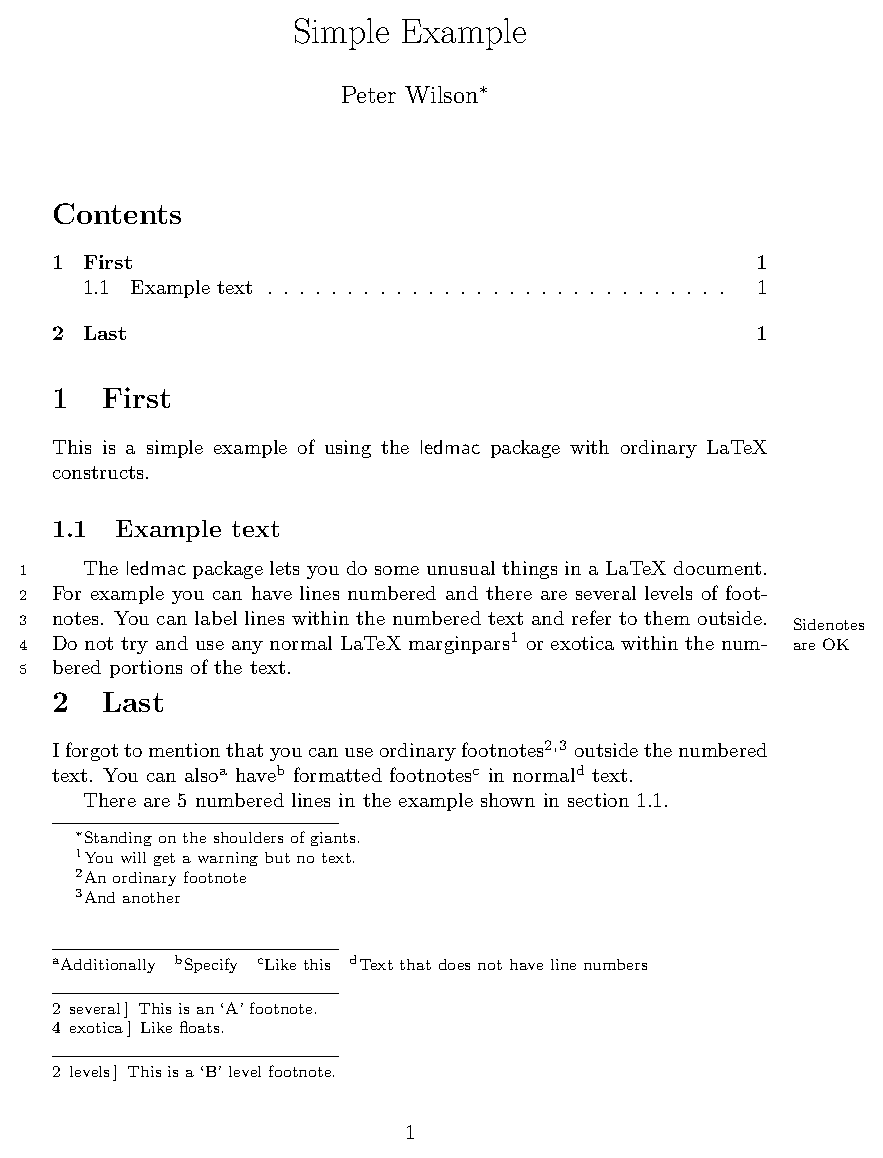
\includegraphics{ledeasy}
% \caption{Output from \texttt{ledeasy.tex}.}
% \label{easy-out}
% \end{figure}
%
% \medskip
% \hrule
% \medskip
%    \begin{macrocode}
%<*easy>
% ledeasy.tex simple example of the ledmac package
\documentclass{article}
\usepackage{ledmac}
%% number every line
\setcounter{firstlinenum}{1}
\setcounter{linenumincrement}{1}
\title{Simple Example}
\author{Peter Wilson\thanks{Standing on the shoulders of giants.}}
\date{}
\begin{document}
\maketitle
\tableofcontents
\section{First}
   This is a simple example of using the \textsf{ledmac} 
package wth ordinary LaTeX constructs.

\subsection{Example text}\label{subsec}

\beginnumbering
\pstart
The \textsf{ledmac} package lets you do some unusual things in
a LaTeX document. For example you can have lines numbered and 
there are  
\edtext{several}{\Afootnote{This is an `A' footnote.}} 
\edtext{levels}{\Bfootnote{This is a `B' level footnote.}}
of footnotes.
You can label lines within the numbered text and refer to them 
outside. Do not try and use any normal LaTeX footnoting or
\edtext{exotica}{\Afootnote{Like floats.}}
within the numbered portions of the text\edlabel{line}.
\pend
\endnumbering

\section{Last}

    I forgot to mention that you can use ordinary 
footnotes\footnote{An ordinary footnote} 
outside the numbered text. There are 
\lineref{line} numbered lines in the example shown 
in section~\ref{subsec}.

\end{document}
%</easy>
%    \end{macrocode}
%
% \end{PW}
%
%
% \subsection{General example of features}
% This made-up example, \verb"ledfeat.tex", is included purely to illustrate
% some of \edmac's main features.  It is hard to find real-world
% examples that actually use as many layers of notes as this, so we made
% one up.  The example is a bit tricky to read, but close study and
% comparison with the output (Figure~\ref{features-out}) will be
% illuminating.
% \begin{figure}[p]
% \centering
% 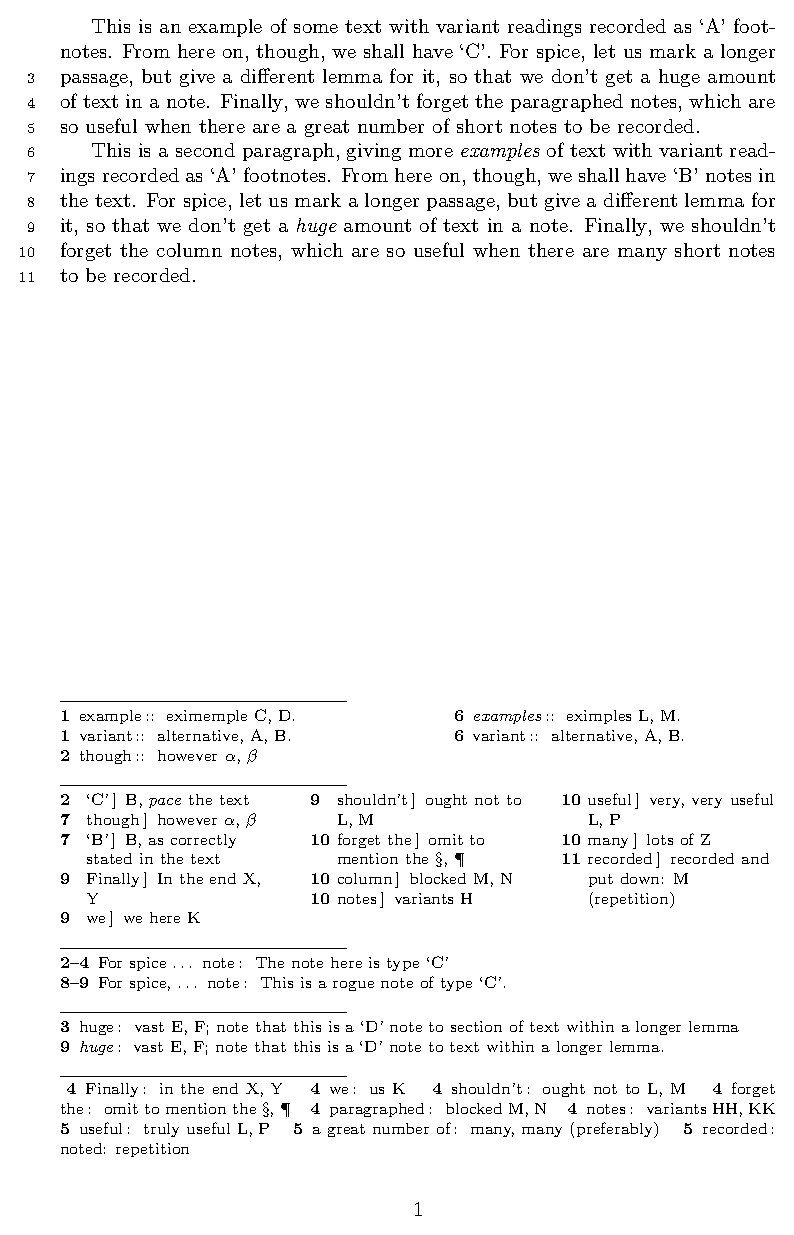
\includegraphics{ledfeat}
% \caption{Output from \texttt{ledfeat.tex}.}
% \label{features-out}
% \end{figure}
%
% \begin{PW}
% I have converted the original TeX code to look more like LaTeX code.
% \end{PW}
%
% \medskip
% \hrule
% \medskip
%    \begin{macrocode}
%<*features>
% ledfeat.tex  Small test file for ledmac package
\documentclass{article}
\usepackage{ledmac}

 \makeatletter
 % I'd like a spaced out colon after the lemma:
 \newcommand{\spacedcolon}{{\rmfamily\thinspace:\thinspace}}
 \renewcommand*{\normalfootfmt}[3]{%
   \normal@pars
   \parindent=0pt \parfillskip=0pt plus 1fil
   {\notenumfont\printlines#1|}\strut\enspace
   {\select@lemmafont#1|#2}\spacedcolon\enskip#3\strut\par}

 % And I'd like the 3-col notes printed with a hanging indent:
 \renewcommand*{\threecolfootfmt}[3]{%
   \normal@pars
   \hsize .3\hsize
   \parindent=0pt
   \tolerance=5000       % high, but not infinite
   \raggedright
   \hangindent1.5em \hangafter1
   \leavevmode
   \strut\hbox to 1.5em{\notenumfont\printlines#1|\hfil}\ignorespaces
   {\select@lemmafont#1|#2}\rbracket\enskip
   #3\strut\par\allowbreak}

 % And I'd like the 2-col notes printed with a double colon:
 \newcommand*{\doublecolon}{{\rmfamily\thinspace::\thinspace}}
 \renewcommand*{\twocolfootfmt}[3]{%
   \normal@pars
   \hsize .45\hsize
   \parindent=0pt
   \tolerance=5000
   \raggedright
   \leavevmode
   \strut{\notenumfont\printlines#1|}\enspace
   {\select@lemmafont#1|#2}\doublecolon\enskip
   #3\strut\par\allowbreak}

 % And in the paragraphed footnotes, I'd like a colon too:
 \renewcommand*{\parafootfmt}[3]{%
   \normal@pars
   \parindent=0pt \parfillskip=0pt plus 1fil
   {\notenumfont\printlines#1|}\enspace
   {\select@lemmafont#1|#2}\spacedcolon\enskip
   #3\penalty-10 }
 \makeatother

 % I'd like the line numbers picked out in bold.
 \renewcommand{\notenumfont}{\bfseries}
 \lineation{page}
 \linenummargin{inner}
 \setcounter{firstlinenum}{3}       % just because I can
 \setcounter{linenumincrement}{1}
 \foottwocol{A}
 \footthreecol{B}
 \footparagraph{E}
 % I've changed \normalfootfmt, so invoke it again for C and D notes.
 \footnormal{C}
 \footnormal{D}

\begin{document}

 \beginnumbering

 \pstart
 This is an \text{example}
   \Afootnote{eximemple C, D.}/
 of some %\footnote{A normal footnote} 
 text with \text{variant}
   \Afootnote{alternative, A, B.}/
 readings recorded as `A' footnotes.  From here on, \text{though}
   \Afootnote{however $\alpha$, $\beta$}/,
 we shall have \text{`C'}
   \Bfootnote{B, \textit{pace} the text}/.
 \text{For spice, let us mark a longer passage, but give a different
   lemma for it, so that we don't get a \text{huge}
     \Dfootnote{vast E, F; note that this is
     a `D' note to section of text within a longer lemma}/
   amount of text in a note}\lemma{For spice \dots\ note}
   \Cfootnote{The note here is type `C'}/.
 \text{Finally}
   \Efootnote{in the end X, Y}/,
 \text{we}
   \Efootnote{us K}/
 \text{shouldn't}
   \Efootnote{ought not to L, M}/
 \text{forget the}
   \Efootnote{omit to mention the \S, \P}/
 \text{paragraphed}
   \Efootnote{blocked M, N}/
 \text{notes}
   \Efootnote{variants HH, KK}/,
 which are so \text{useful}
   \Efootnote{truly useful L, P}/
 when there are \text{a great number of}
   \Efootnote{many, many (preferably)}/
 short notes to be \text{recorded}
   \Efootnote{noted: repetition}/.
 \pend

%    \end{macrocode}
% \begin{PW}
% For comparison purposes, the second paragraph uses the \cs{edtext}
% macro rather than the \cs{text} macro.
% \end{PW}
%    \begin{macrocode}
 \pstart
 This is a second paragraph, giving more \textit{\edtext{examples}{
   \Afootnote{eximples L, M.}}}
 of text with \edtext{variant}{
   \Afootnote{alternative, A, B.}}
 readings recorded as `A' footnotes.  From here on, \edtext{though}{
   \Bfootnote{however $\alpha$, $\beta$}},
 we  shall have \edtext{`B'}{
   \Bfootnote{B, as correctly stated in the text}} notes in the text.
 \edtext{For spice, let us mark a longer passage, but give a different
   lemma for it, so that we don't get a \textit{\edtext{huge}{
     \Dfootnote{vast E, F; note that this is
     a `D' note to text within a longer lemma.}}}
   amount of text in a note}{\lemma{For spice, \dots\ note}
   \Cfootnote{This is a rogue note of type `C'.}}.
 \edtext{Finally}{
   \Bfootnote{In the end X, Y}},
 \edtext{we}{
   \Bfootnote{we here K}}
 \edtext{shouldn't}{
   \Bfootnote{ought not to L, M}}
 \edtext{forget the}{
   \Bfootnote{omit to mention the \S, \P}}
 \edtext{column}{
   \Bfootnote{blocked M, N}}
 \edtext{notes}{
   \Bfootnote{variants H}},
 which are so \edtext{useful}{
   \Bfootnote{very, very useful L, P}}
 when there are \edtext{many}{
   \Bfootnote{lots of Z}}
 short notes to be \edtext{recorded}{
   \Bfootnote{recorded and put down: M (repetition)}}.
 \pend

 \endnumbering
\end{document}
%</features>
%    \end{macrocode}
% \medskip
% \hrule
% \medskip
%
% \subsection{Gascoigne}
% The first real-life example is taken from an edition of George
% Gascoigne's {\em A Hundreth Sundrie Flowres\/} that is being
% prepared by G.~W.~Pigman III,\index{Pigman, III$^{rd}$, G. W.} at
% the California Institute of Technology. Figure \ref{iocasta-out}
% shows the result of setting the text with \edmac.
% \begin{figure}[p]
% \centering
% 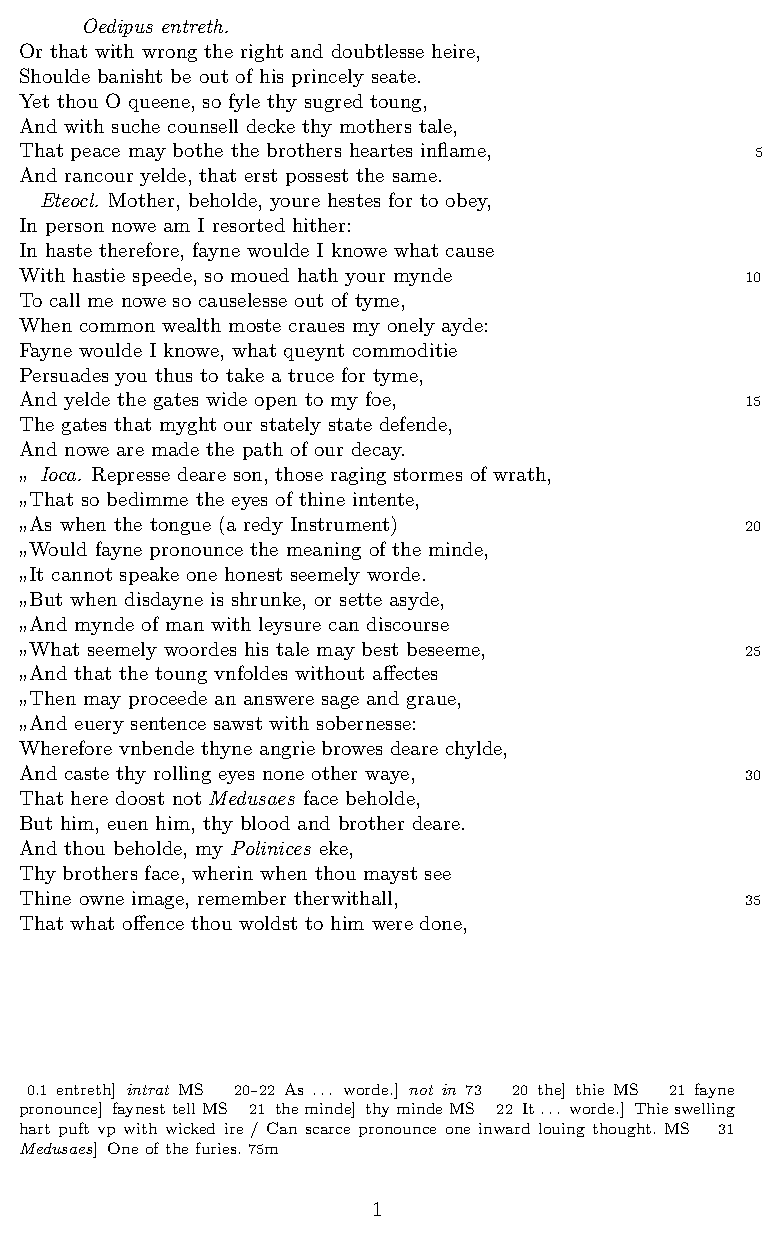
\includegraphics{ledioc}
% \caption{Output from \texttt{ledioc.tex}.}
% \label{iocasta-out}
% \end{figure}
%
% \iffalse
%
% The main input file first calls for a file of initial
% definitions, called \verb"gg.tex".  This file, shown below,
% demonstrates how \edmac{} macros may be customized to give
% detailed control over the final format.
%
% \fi
%
% \begin{PW}
% I have LaTeXified the original code, and removed all the code related
% to the main document layout, relying on the standard LaTeX layout parameters..
% \end{PW}
%
% \medskip
%
% \hrule
% \medskip
%    \begin{macrocode}
%<*ioc>
%% ledioc.tex  
\documentclass{article}
\usepackage{ledmac}

 \noendnotes
 \makeatletter

 \newcommand{\os}{\scriptsize}
 \setcounter{firstsublinenum}{1000}
 \frenchspacing \parskip=0pt \hyphenpenalty=1000

 % Say \nolinenums if you want no line numbers in the notes.
 \newif\ifnolinenums
 \newcommand{\nolinenums}{\global\nolinenumstrue}
 \newcommand{\linenums}{\global\nolinenumsfalse}

 \renewcommand{\rightlinenum}{\ifbypage@\ifnum\line@num<10\kern.5em\fi\else
 \ifnum\line@num<10\kern1em\else\ifnum\line@num<100
   \kern.5em\fi\fi\fi\kern.5em\numlabfont\the\line@num
   \ifnum\subline@num>0:\the\subline@num\fi}

 \renewcommand{\leftlinenum}{\numlabfont\the\line@num
   \ifnum\subline@num>0:\the\subline@num\fi \kern.5em}
 \linenummargin{outer}
 \lineation{page}

 \newcommand{\ggfootfmt}[3]{%
   \notefontsetup
   \let\par=\endgraf
   \rightskip=0pt \leftskip=0pt
   \parindent=0pt \parfillskip=0pt plus 1fil
   \ifnolinenums\relax\else
     \begingroup \os \printlines#1|\endgroup
     \enskip
   \fi
   {\rmfamily #2\def\@tempa{#2}\ifx\@tempa\empty
     \else]\enskip\fi#3\penalty-10 }}

 % Now reset the \Afootnote parameters and macros:
 \footparagraph{A}
 \let\Afootfmt=\ggfootfmt
 \dimen\Afootins=\vsize
 \skip\Afootins=3pt plus9pt
 \newcommand*{\ggfootstart}[1]{\vskip\skip\Afootins}
 \let\Afootstart=\ggfootstart

 \newcommand*{\stage}[1]{\pstart\startsub\parindent=0pt
   \hangindent=3em\hangafter=0
   {\itshape #1}\let\par=\finishstage}
 \newcommand{\finishstage}{\pend\endsub}
 \newcommand{\sen}{\leavevmode\lower1ex\hbox{\textrm{''}}}
 \newcommand{\senspeak}[1]{\pstart\obeylines\setbox0=\hbox{\textrm{''}}%
   \leavevmode
   \lower1ex\copy0\kern-\wd0\hskip1em{\textit{#1}}%
   \hbox to1ex{}\ignorespaces}
 \newcommand*{\speak}[1]{\pstart\obeylines\hskip1em{\textit{#1}}%
   \hbox to1ex{}\ignorespaces}
 \def\nospeaker{\parindent=0em\pstart\let\par=\pend}
 \newcommand*{\nospeak}{\pstart\obeylines}
 \makeatother

\begin{document}

 \setlength{\parindent}{0pt}

 \beginnumbering

 \stage{Oedipus \edtext{entreth}{\Afootnote{\textit{intrat} MS}}.}

 \nospeak
 Or that with wrong the right and doubtlesse heire,
 Shoulde banisht be out of his princely seate.
 Yet thou O queene, so fyle thy sugred toung,
 And with suche counsell decke thy mothers tale,
 That peace may bothe the brothers heartes inflame,
 And rancour yelde, that erst possest the same.
 \pend

 \speak{Eteocl.} Mother, beholde, youre hestes for to obey,
 In person nowe am I resorted hither:
 In haste therefore, fayne woulde I knowe what cause
 With hastie speede, so moued hath your mynde
 To call me nowe so causelesse out of tyme,
 When common wealth moste craues my onely ayde:
 Fayne woulde I knowe, what queynt commoditie
 Persuades you thus to take a truce for tyme,
 And yelde the gates wide open to my foe,
 The gates that myght our stately state defende,
 And nowe are made the path of our decay.
 \pend

 \senspeak{Ioca.}Represse deare son, those raging stormes of wrath,
 \sen That so bedimme the eyes of thine intente,
 \edtext{\sen As when \edtext{the}{\Afootnote{thie MS}} tongue %
   (a redy Instrument)
 \sen Would \edtext{fayne pronounce}{\Afootnote{faynest tell MS}} %
   the meaning of \edtext{the minde}{\Afootnote{thy minde MS}},
 \sen \edtext{It}{\lemma{It \dots\ worde.}\Afootnote{Thie %
   swelling hart puft vp with wicked ire / Can scarce pronounce %
   one inward louing thought. MS}} cannot speake one honest %
   seemely worde.}{\lemma{As \dots\ worde.}\Afootnote{\textit{not %
   in} \os73}}
 \sen But when disdayne is shrunke, or sette asyde,
 \sen And mynde of man with leysure can discourse
 \sen What seemely woordes his tale may best beseeme,
 \sen And that the toung vnfoldes without affectes
 \sen Then may proceede an answere sage and graue,
 \sen And euery sentence sawst with sobernesse:
 Wherefore vnbende thyne angrie browes deare chylde,
 And caste thy rolling eyes none other waye,
 That here doost not \edtext{\textit{Medusaes}}{%
 \Afootnote{One of the furies. {\os75}m}} face beholde,
 But him, euen him, thy blood and brother deare.
 And thou beholde, my \textit{Polinices} eke,
 Thy brothers face, wherin when thou mayst see
 Thine owne image, remember therwithall,
 That what offence thou woldst to him were done,
 \pend
 \endnumbering

\end{document}

%</ioc>
%    \end{macrocode}
% \medskip
% \hrule
%
% \subsection{Shakespeare}
% The following text illustrates another input file of moderate
% complexity, with two layers of annotation in use. The example is
% taken from the Arden {\em Merchant of Venice}.\index{Shakespeare, William}
%
% \iffalse
%
% First, the file \verb"arden.sty" contains a set of font
% definitions and format specifications:
%
% The Arden text, using the above definitions, is input as follows
% (the output is shown in Figure \ref{arden-out}):
%
% \fi
%
% \begin{PW}
% I have roughly converted the original TeX file to a LaTeX file.
% The file is below and the result of LaTeXing it is shown in
% Figure~\ref{arden-out}.
% \end{PW}
%
% \begin{figure}[p]
% \centering
% 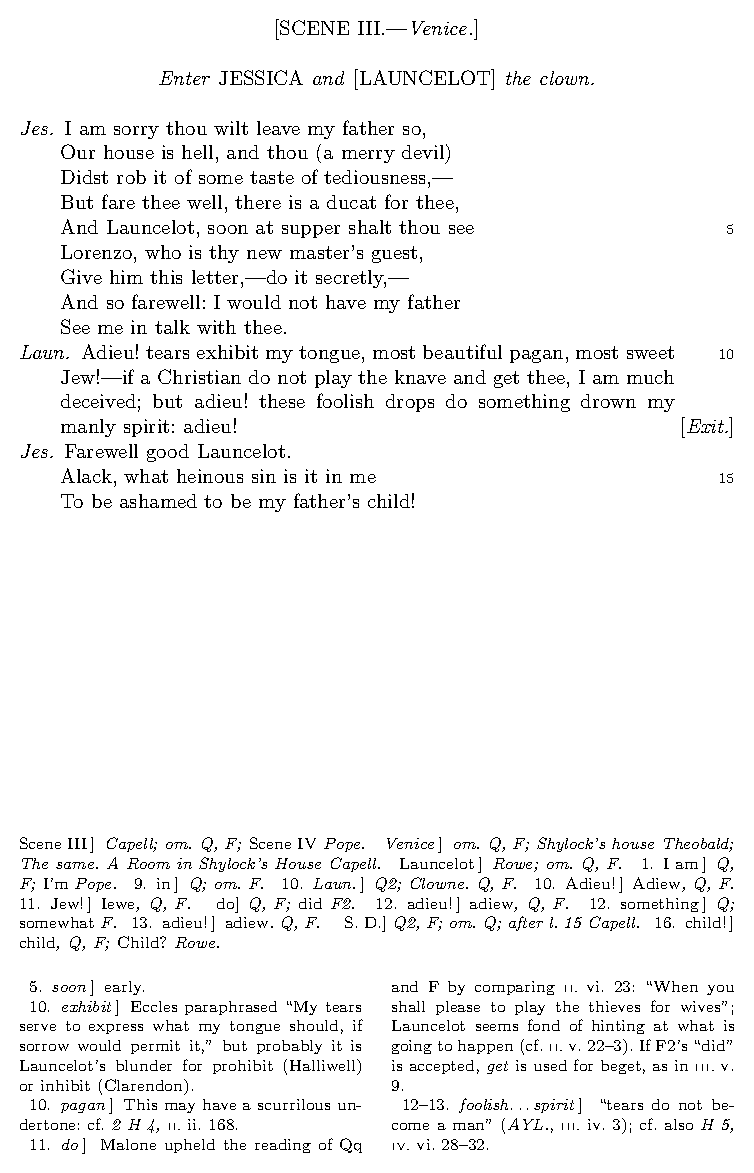
\includegraphics{ledarden}
% \caption{Output from \texttt{ledarden.tex}.}
% \label{arden-out}
% \end{figure}
%
%
% \medskip
% \hrule
% \medskip
%
%    \begin{macrocode}
%<*arden>
%% ledarden.tex
\documentclass{article}
\usepackage{ledmac}

\makeatletter
 \newcommand{\stage}[1]{\rlap{\hbox to \the\linenumsep{%
                        \hfil\llap{[\textit{#1}]}}}}

 \newcommand{\speaker}[1]{\pstart\hangindent2em\hangafter1
   \leavevmode\textit{#1}\enspace\ignorespaces}

 \newcommand{\exit}[1]{\hfill\stage{#1}}

 % EDMAC customizations:
 \noendnotes 
 \vsize 40pc 
 \hsize 23pc 
 \parindent 0pt
 \linenumsep=.4in 
 \rightskip\linenumsep

 \renewcommand{\interparanoteglue}{1em plus.5em minus.1em}

 \catcode`\<=\active
 \def\xtext#1#2>{\text{#1}{#2}/}
 \let<=\xtext

 \newcommand{\scf}{\tiny}
 \let\Afootnoterule=\relax \let\Bfootnoterule=\relax

 \renewcommand{\rightlinenum}{\numlabfont\llap{\the\line@num}}
 \frenchspacing

 % Footnote formats:
 % \nonumparafootfmt is a footnote format without line numbers.
 \newcommand{\nonumparafootfmt}[3]{%
   \normal@pars
   \rightskip=0pt
   \parindent=0pt \parfillskip=0pt plus 1fil
   \select@lemmafont#1|#2\rbracket\enskip
   \it#3\penalty-10 }

 \newcommand{\newparafootfmt}[3]{%
   \normal@pars
   \parindent=0pt \parfillskip=0pt plus 1fil
   {\notenumfont\printlines#1|}\fullstop\enspace
   {\select@lemmafont#1|#2}\rbracket\enskip
   \it#3\penalty-10 }

 \newcommand{\newtwocolfootfmt}[3]{%
   \normal@pars
   \hsize .48\hsize
   \tolerance=5000
   \rightskip=0pt \leftskip=0pt \parindent=5pt
   \strut\notenumfont\printlines#1|\fullstop\enspace
   \it#2\/\rbracket\penalty100\hskip .5em plus .5em
   \rm#3\strut\goodbreak}

 % Footnote style selections etc. (done last):
 \footparagraph{A}
 \foottwocol{B}
 \let\Afootfmt=\newparafootfmt
 \let\Bfootfmt=\newtwocolfootfmt
 \let\collation=\Afootnote
 \let\note=\Bfootnote
 \lineation{section}
 \linenummargin{right}
 \makeatother

%%%%%%%%%%%%%%%%%%%%%%%%%%%%%%%%

\begin{document}
 \pagestyle{empty}

 % Initially, we don't want line numbers.
 \let\Afootfmt=\nonumparafootfmt

 \beginnumbering
 \pstart
 \centerline{[<{SCENE III}
   \lemma{Scene III}
   \collation{Capell; om. Q, F; \textnormal{Scene IV} Pope.}>.---%
   <{\textit{Venice}}
   \collation{om. Q, F; Shylock's house Theobald; The same.
   A Room in Shylock's House Capell.}>.]}
 \pend
 \bigskip

 \pstart
 \centerline{\textit{Enter} JESSICA \textit{and}
   [<{LAUNCELOT}
   \lemma{Launcelot}
   \collation{Rowe; om. Q, F.}>] \textit{the clown.}} \pend \bigskip

 \let\Afootfmt=\newparafootfmt % we do want line numbers from now

  \setline{0}%

 \speaker{Jes.}<{I am}
   \collation{Q, F; \textnormal{I'm} Pope.}>
                       sorry thou wilt leave my father so,\\
 Our house is hell, and thou (a merry devil)\\
 Didst rob it of some taste of tediousness,---\\
 But fare thee well, there is a ducat for thee,\\
 And Launcelot, <{soon}
   \note{early.}>
                        at supper shalt thou see\\
 Lorenzo, who is thy new master's guest,\\
 Give him this letter,---do it secretly,---\\
 And so farewell: I would not have my father\\
 See me <{in}
   \collation{Q; om. F.}>
              talk with thee.
 \pend

 \speaker{Laun.}
   <{}\lemma{\it Laun.}\collation{Q2; Clowne. Q, F.}>%
 <{Adieu!}
   \collation{\textnormal{Adiew}, Q, F.}>
 tears <{exhibit}
   \note{Eccles paraphrased ``My tears serve to express what my
   tongue should, if sorrow would permit it,'' but probably it is
   Launce\-lot's blunder for prohibit (Halliwell) or inhibit
   (Clarendon).}>
 my tongue, most beautiful <{pagan}
   \note{This may have a scurrilous undertone: cf. \textit{2 H 4,}
   {\scf II.} \textrm{ii. 168.}}>%
 , most sweet <{Jew!}
   \collation{\textnormal{Iewe}, Q, F. \quad \textnormal{do]} Q, F;
              \textnormal{did} F2.}>%
 ---if a Christian <{do}
   \note{Malone upheld the reading of Qq and F by comparing {\scf II.}
    vi. 23: ``When you shall please to play the thieves for
   wives''; Launcelot seems fond of hinting at what is going to
   happen (cf. {\scf II.} v. 22--3). If F2's ``did'' is accepted,
   \textit{get} is used for beget, as in {\scf III.} v. 9.}>
 not play the knave and get thee, I am much deceived; but <{adieu!}
   \collation{\textnormal{adiew}, Q, F.}>
 these <{foolish drops do \text{something}
   \collation{Q; \textnormal{somewhat} F.}/
 drown my manly spirit}
   \lemma{foolish\textnormal{\dots}spirit}
   \note{``tears do not become a man'' (\textit{AYL.}, {\scf III.} 
   iv. 3); cf. also \textit{H 5,} {\scf IV.} vi. 28--32.}>%
 : <{adieu!}
   \collation{\textnormal{adiew}. Q, F. \quad \textnormal{S. D.]} Q2, F; om. Q;
   after l. 15 Capell.}>
 \exit{Exit.}
 \pend

 \speaker{Jes.}
 Farewell good Launcelot.\\
 Alack, what heinous sin is it in me\\
 To be ashamed to be my father's <{child!}
   \collation{\textnormal{child}, Q, F; \textnormal{Child?} Rowe.}>
 \pend
 \endnumbering

\end{document}

%</arden>
%    \end{macrocode}
%
% \medskip
% \hrule
%
% \subsection{Classical text edition}
% The next example, which was extracted from a longer file kindly
% supplied by Wayne Sullivan,\index{Sullivan, Wayne} University
% College, Dublin, Ireland, illustrates the use of \edmac{} to
% produce a Latin text edition, the {\em Periphyseon}, with Greek
% passages.\footnote{The bibliographic details of the forthcoming book
% are: Iohannis Scotti Erivgenae, {\it Periphyseon} ({\it De
% Diuisione Naturae\/}) Liber Qvartvs [Scriptores Latini Hiberniae
% vol.\,xii], (Dublin: School of Celtic Studies, Dublin Institute
% for Advanced Studies, forthcoming 1992).}  The Greek font used is
% that prepared by Silvio Levy\index{Levy, Silvio} and described in {\em
% TUGboat}.\footnote{{\em TUGboat\/} {\bf 9} (1988), pp.\,20--24.} The
% output of this file is shown in Figure~\ref{periphyseon-out}.
% Note the use of two layers of footnotes to record testimonia and
% manuscript readings respectively.
%
% \begin{PW}
%  I have converted the original \edmac{} example file from TeX
% to something that looks more like LaTeX.
% \end{PW}
%
% ^^A Periphyseon, Liber IV
%
% \begin{figure}[p]
% \centering
% \hspace*{-2in}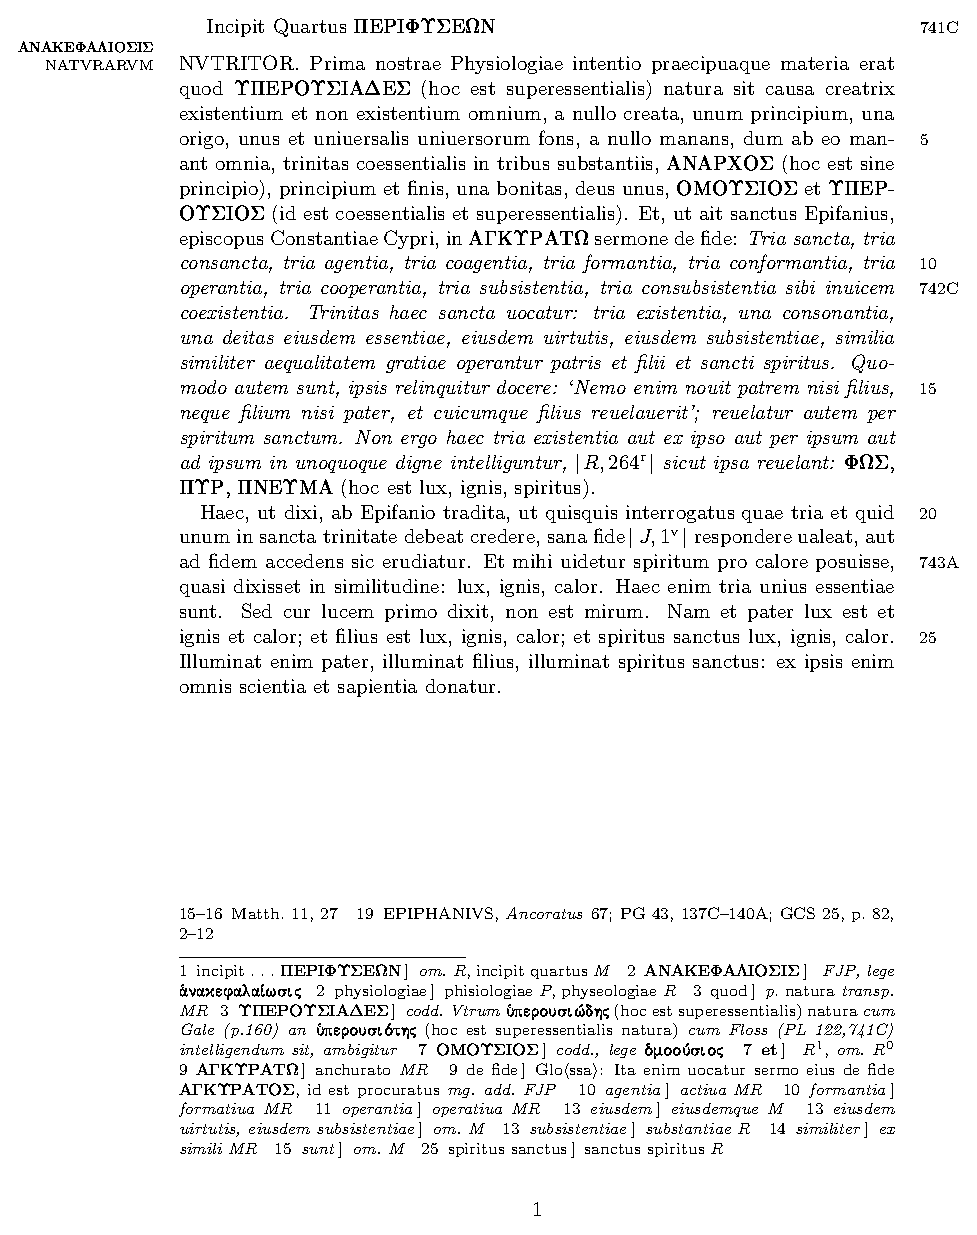
\includegraphics{ledmixed}\hspace*{-2in}
% \caption{Output from \texttt{ledmixed.tex}.}
% \label{periphyseon-out}
% \end{figure}
%
%
% \medskip
% \hrule
% \medskip
%
%    \begin{macrocode}
%<*periph>
% ledmixed.tex
\documentclass{article}
\usepackage{ledmac}

 \overfullrule0 pt
 \lefthyphenmin=3

%    \end{macrocode}
% \begin{PW}
% The LaTeX version uses the \Lpack{lgreek} package to access Silvio Levy's
% greek font. The \texttt{delims} package option 
% subverts\footnote{It actually changes its category code.} the normal meaning
% of \$ to switch in and out of math mode. We have to save the original meaning
% of \$ before calling the package. Later, we use \cs{Ma} and \cs{aM} for math mode
% switching.
% \end{PW}
%    \begin{macrocode}
\let\Ma=$
\let\aM=$
\usepackage[delims]{lgreek}

 % We need an addition to \no@expands since the \active $ in lgreek
 % causes problems:
 \newcommand{\morenoexpands}{\let$=0}

\makeatletter

 \newbox\lp@rbox

 \newcommand{\ffootnote}[1]{%
   \ifnumberedpar@
     \xright@appenditem{\noexpand\vffootnote{f}{{\@nums}{\@tag}{#1}}}%
                                                 \to\inserts@list
     \global\advance\insert@count by 1
 %  \else         %% may be used only in numbered text
 %    \vffootnote{f}{{0|0|0|0|0|0|0}{}{#1}}%
   \fi\ignorespaces}

 \newcommand{\gfootnote}[1]{%
   \ifnumberedpar@
     \xright@appenditem{\noexpand\vgfootnote{g}{#1}}%
                                                 \to\inserts@list
     \global\advance\insert@count by 1
 %  \else         %% may be used only in numbered text
 %    \vgfootnote{g}{#1}%
   \fi\ignorespaces}

 \newcommand{\setlp@rbox}[3]{%
   {\parindent\z@\hsize=2.5cm\raggedleft\eightpoint
   \baselineskip 9pt%
   \global\setbox\lp@rbox=\vbox to\z@{\vss#3}}}

 \newcommand{\vffootnote}[2]{\setlp@rbox#2}

 \newcommand{\vgfootnote}[2]{\def\rd@ta{#2}}

 \renewcommand{\do@line}{%
  {\vbadness=10000 \splittopskip=0pt
  \gdef\rd@ta{}% for right margin paragraph->always a few characters
  \global\setbox\one@line=\vsplit\raw@text to\baselineskip}%
  \unvbox\one@line \global\setbox\one@line=\lastbox
  \getline@num
 \hbox to\hsize{\affixline@num\add@inserts\hbox to\z@% inserts added here so
   {\hss\box\lp@rbox\kern\linenumsep}%                 that margin pars are
    \hfil\hbox to\wd\one@line{\new@line\unhbox\one@line%   included.
       \hbox to\z@{\kern\linenumsep\notenumfont\rd@ta\hss}}}%
  \add@penalties} % margin pars also included in line format

 \renewcommand{\affixline@num}{%
   \ifsublines@
     \@tempcntb=\subline@num
     \ifnum\subline@num>\c@firstsublinenum
       \@tempcnta=\subline@num
       \advance\@tempcnta by-\c@firstsublinenum
       \divide\@tempcnta by\c@sublinenumincrement
       \multiply\@tempcnta by\c@sublinenumincrement
       \advance\@tempcnta by\c@firstsublinenum
     \else
       \@tempcnta=\c@firstsublinenum
     \fi
     %
     \ifcase\sub@lock
       \or
         \ifnum\sublock@disp=1
            \@tempcntb=0 \@tempcnta=1
         \fi
       \or
         \ifnum\sublock@disp=2 \else
            \@tempcntb=0 \@tempcnta=1
         \fi
       \or
         \ifnum\sublock@disp=0
            \@tempcntb=0 \@tempcnta=1
         \fi
     \fi
   \else
     \@tempcntb=\line@num
     \ifnum\line@num>\c@firstlinenum
        \@tempcnta=\line@num
        \advance\@tempcnta by-\c@firstlinenum
        \divide\@tempcnta by\c@linenumincrement
        \multiply\@tempcnta by\c@linenumincrement
        \advance\@tempcnta by\c@firstlinenum
     \else
        \@tempcnta=\c@firstlinenum
     \fi
     \ifcase\@lock
        \or
          \ifnum\lock@disp=1
             \@tempcntb=0 \@tempcnta=1
          \fi
        \or
          \ifnum\lock@disp=2 \else
             \@tempcntb=0 \@tempcnta=1
          \fi
        \or
          \ifnum\lock@disp=0
             \@tempcntb=0 \@tempcnta=1
          \fi
     \fi
   \fi
   %
   \ifnum\@tempcnta=\@tempcntb
     \@tempcntb=\line@margin
     \ifnum\@tempcntb>1
       \advance\@tempcntb by\page@num
     \fi
     \ifodd\@tempcntb
 %      #1\rlap{{\rightlinenum}}%
        \xdef\rd@ta{\the\line@num}%
     \else
       \llap{{\leftlinenum}}%#1%
     \fi
   \else
     %#1%
   \fi
   \ifcase\@lock
   \or
     \global\@lock=2
   \or \or
     \global\@lock=0
   \fi
   \ifcase\sub@lock
   \or
     \global\sub@lock=2
   \or \or
     \global\sub@lock=0
   \fi}

\newcommand{\eightpoint}{\scriptsize}

 \lineation{page}
 \linenummargin{right}
 \footparagraph{A}
 \footparagraph{B}

\renewcommand{\notenumfont}{\footnotesize}
\newcommand{\notetextfont}{\footnotesize}

 \let\Afootnoterule=\relax
 \count\Afootins=825
 \count\Bfootins=825

 \newcommand{\Aparafootfmt}[3]{%
   \normal@pars\eightpoint
   \parindent=0pt \parfillskip=0pt plus1fil
   \notenumfont\printlines#1|\enspace
 %      \lemmafont#1|#2\enskip
   \notetextfont
   #3\penalty-10\hskip 1em plus 4em minus.4em\relax}

 \newcommand{\Bparafootfmt}[3]{%
   \normal@pars\eightpoint
   \parindent=0pt \parfillskip=0pt plus1fil
   \notenumfont\printlines#1|\enspace
   \select@lemmafont#1|#2\rbracket\enskip
   \notetextfont
   #3\penalty-10\hskip 1em plus 4em minus.4em\relax }
 \makeatother

 \let\Afootfmt=\Aparafootfmt
 \let\Bfootfmt=\Bparafootfmt
 \def\lemmafont#1|#2|#3|#4|#5|#6|#7|{\eightpoint}
 \parindent=1em

 \newcommand{\lmarpar}[1]{\text{}\ffootnote{#1}/}

 \newcommand{\rmarpar}[1]{\text{}\gfootnote{#1}/}
 \emergencystretch40pt

%%%%%%%%%%%%%%%%%%%%%%%%%%%%%%%%%%%%%%%%%%%%%%

\begin{document}

 \beginnumbering
 \pstart
 \rmarpar{741C}
 \noindent \text{Incipit Quartus $PERIFUSEWN$}%
 \lemma{incipit\ .~.~.\ $PERIFUSEWN$}\Bfootnote{\textit{om.\ R},
 incipit quartus \textit{M}}/
 \pend
 \medskip

 \pstart
 \noindent \text{NVTRITOR}\lemma{$ANAKEFALIOSIS$}\Bfootnote{\textit{
 FJP, lege} $<anakefala'iwsis$}/.\lmarpar{$ANAKEFALIOSIS$
 NATVRARVM} Prima nostrae
 \text{Physiologiae}\lemma{physiologiae}\Bfootnote{phisiologiae
 \textit{P}, physeologiae \textit{R}}/ intentio praecipuaque mat\-e\-ria
 erat \text{quod}\Bfootnote{\textit{p}.\ natura \textit{transp.\ MR}}/
 \text{$UPEROUSIADES$}\Bfootnote{\textit{codd.\ Vtrum}
 $<uperousi'wdhs$ (hoc est superessentialis) natura \textit{cum Gale
 (p.160) an} $<uperousi'oths$ (hoc est superessentialis natura)
 \textit{cum Floss (PL 122,741C) intelligendum sit, ambigitur}}/ (hoc
 est superessentialis) natura sit causa creatrix existentium et
 non existentium omnium, a nullo creata, unum principium, una
 origo, unus et uniuersalis uniuersorum fons, a nullo manans, dum
 ab eo manant omnia, trinitas coessentialis in tribus substantiis,
 $ANARQOS$ (hoc est sine principio), principium et finis, una
 bonitas, deus unus, \text{$OMOUSIOS$}\Bfootnote{\textit{codd.,
 lege} $<omoo'usios$}/ \text{et}\lemma{\textbf{et}}\Bfootnote{\textit{
 R}\textsuperscript{1}, \textit{om.\ R}\textsuperscript{0}}/
 $UPEROUSIOS$ (id est coessentialis et superessentialis). Et, ut
 ait sanctus Epifanius, episcopus Constantiae Cypri, in
 \text{$AGKURATW$}\Bfootnote{anchurato \textit{MR}}/ sermone \text{de
 fide}\Bfootnote{Glo\Ma\langle\aM ssa\Ma\rangle\aM: Ita
 enim uocatur sermo eius de fide $AGKURATOS$, id est procuratus
 \textit{mg.\ add.\ FJP}}/: 
 \begin{itshape}Tria sancta, tria consancta, tria
 \text{agentia}\Bfootnote{actiua \textit{MR}}/, tria coagentia, tria
 \text{formantia}\Bfootnote{formatiua \textit{MR}}/, tria
 conformantia, tria \text{operantia}\Bfootnote{operatiua \textit{MR}}/,
 tria cooperantia, tria subsistentia, tria\rmarpar{742C}
 consubsistentia sibi inuicem coexistentia. Trinitas haec
 sancta uocatur: tria existentia, una consonantia, una deitas
 \text{eiusdem}\Bfootnote{eiusdemque \textit{M}}/ essentiae,
 \text{eiusdem uirtutis, eiusdem
 \text{subsistentiae}{\Bfootnote{substantiae \textit{R}}}/}%
 \Bfootnote{\textit{om.\ M}}/, similia \text{similiter}\Bfootnote{ex
 simili \textit{MR}}/ aequalitatem gratiae operantur patris et filii
 et sancti spiritus. Quomodo autem \text{sunt}\Bfootnote{\textit{om.\
 M}}/, ipsis relinquitur docere: \text{`Nemo enim nouit patrem
 nisi filius, neque filium nisi pater, et cuicumque filius
 reuelauerit'}\Afootnote{Matth.\ 11, 27}/; reuelatur autem per
 spiritum sanctum. Non ergo haec tria existentia aut ex ipso aut
 per ipsum aut ad ipsum in unoquoque digne intelliguntur,
 \Ma\mid\! R, 264^{\rm r}\!\mid\aM\ sicut ipsa reuelant:\end{itshape}
 $FWS, PUR, PNEUMA$ \text{(hoc est lux, ignis,
 spiritus)}\Afootnote{EPIPHANIVS, \textit{Ancoratus} 67; PG~43,
 137C--140A; GCS 25, p.~82, 2--12}/.
 \pend

 \pstart
 Haec, ut dixi, ab Epifanio tradita, ut quisquis interrogatus quae
 tria et quid unum in sancta trinitate debeat credere, sana fide
 \Ma\!\mid J, 1^{\rm v}\!\mid\aM\ respondere ualeat, aut ad
 fidem accedens\rmarpar{743A} sic erudiatur. Et mihi uidetur
 spiritum pro calore posuisse, quasi dixisset in similitudine:
 lux, ignis, calor. Haec enim tria unius essentiae sunt. Sed cur
 lucem primo dixit, non est mirum. Nam et pater lux est et ignis
 et calor; et filius est lux, ignis, calor; et \text{spiritus
 sanctus}\Bfootnote{sanctus spiritus \textit{R}}/ lux, ignis, calor.
 Illuminat enim pater, illuminat filius, illuminat spiritus
 sanctus: ex ipsis enim omnis scientia et sapientia donatur.
 \pend
 \endnumbering

\end{document}

%</periph>
%    \end{macrocode}
%
% \medskip
% \hrule
%
% ^^A PW: I have removed the bits of the Arabic and Sanskrit examples.
% ^^A PW: the iffalse ... fi trick doesn't work here because of embedded ifs
%
%
%
% \Finale
% \PrintIndex
% \endinput
\endinput

%% \CharacterTable
%%  {Upper-case    \A\B\C\D\E\F\G\H\I\J\K\L\M\N\O\P\Q\R\S\T\U\V\W\X\Y\Z
%%   Lower-case    \a\b\c\d\e\f\g\h\i\j\k\l\m\n\o\p\q\r\s\t\u\v\w\x\y\z
%%   Digits        \0\1\2\3\4\5\6\7\8\9
%%   Exclamation   \!     Double quote  \"     Hash (number) \#
%%   Dollar        \$     Percent       \%     Ampersand     \&
%%   Acute accent  \'     Left paren    \(     Right paren   \)
%%   Asterisk      \*     Plus          \+     Comma         \,
%%   Minus         \-     Point         \.     Solidus       \/
%%   Colon         \:     Semicolon     \;     Less than     \<
%%   Equals        \=     Greater than  \>     Question mark \?
%%   Commercial at \@     Left bracket  \[     Backslash     \\
%%   Right bracket \]     Circumflex    \^     Underscore    \_
%%   Grave accent  \`     Left brace    \{     Vertical bar  \|
%%   Right brace   \}     Tilde         \~}
%%
